
\documentclass[11pt]{report}

%% PACKAGES
\usepackage{graphicx}
\usepackage{verbatim}
\usepackage{url}
\usepackage[printonlyused]{acronym}
\usepackage[ruled]{algorithm}
\usepackage{amsmath,amssymb,amsfonts,amsthm}
\usepackage{overpic}
\usepackage{calc}
\usepackage{color}
 \usepackage[margin=1.0in]{geometry}
\usepackage[colorlinks=false]{hyperref}
\usepackage{textcomp}
\usepackage{cite}
\usepackage{mdwlist}
\usepackage{subfiles}
\usepackage{enumitem}
\usepackage{calc}
\usepackage{array}
\usepackage{units}
\usepackage{arydshln,leftidx,mathtools}
\usepackage[caption=false,font=footnotesize]{subfig}
\usepackage{relsize}
\usepackage{float}
\usepackage{makecell}
\usepackage{xr}
\usepackage{multirow}

\usepackage{algorithm}
\usepackage[noend]{algpseudocode}

\usepackage{nicematrix,tikz}
\NiceMatrixOptions
{
  cell-space-limits = 1.25pt, 
  custom-line = 
   {
	 command = ThickHline ,
	 letter = T ,
	 tikz = { color = black, line width = 1.5 pt }
   },
   custom-line = 
   {
	 command = MedHline ,
	 letter = I ,
	 tikz = { color = black, line width = 1.25 pt }
   }
}



\setcounter{secnumdepth}{3}

\makeatletter
\let\@tmp\@xfloat     
\usepackage{fixltx2e}
\let\@xfloat\@tmp                    
\makeatother

\usepackage[subfigure]{tocloft}
\usepackage[singlespacing]{setspace}

\usepackage{pgfplots}
\pgfplotsset{compat=1.18}
\usepackage{cancel}

\usepackage{tikz}
\usetikzlibrary{calc,patterns,decorations.pathmorphing,decorations.markings,fit,backgrounds}

\usepackage[strict]{changepage} %use to manually place figs/tables to get them within the margins

\makeatletter
\g@addto@macro\normalsize{%
  \setlength\abovedisplayskip{0.25pt}
  \setlength\belowdisplayskip{0.25pt}
  \setlength\abovedisplayshortskip{0.25pt}
  \setlength\belowdisplayshortskip{0.25pt}
}
\makeatother



\setlength{\parskip}{\baselineskip}

%% GRAPHICS PATH
\graphicspath{{./pictures/pdf/}{./pictures/ps/}{./pictures/png/}}

%% TODO
\newcommand{\todo}[1]{\vspace{5 mm}\par \noindent \framebox{\begin{minipage}[c]{0.98 \columnwidth} \ttfamily\flushleft \textcolor{red}{#1}\end{minipage}}\vspace{5 mm}\par}


%% MACROS
\providecommand{\abs}[1]{\lvert#1\rvert}
\providecommand{\norm}[1]{\lVert#1\rVert}
\providecommand{\dualnorm}[1]{\norm{#1}_\ast}
\providecommand{\set}[1]{\lbrace\,#1\,\rbrace}
\providecommand{\cset}[2]{\lbrace\,{#1}\nobreak\mid\nobreak{#2}\,\rbrace}
\providecommand{\onevect}{\mathbf{1}}
\providecommand{\zerovect}{\mathbf{0}}
\providecommand{\field}[1]{\mathbb{#1}}
\providecommand{\C}{\field{C}}
\providecommand{\R}{\field{R}}
\providecommand{\polar}{\triangle}
\providecommand{\Cspace}{\mathcal{Q}}
\providecommand{\Fspace}{\mathcal{F}}
\providecommand{\free}{\text{\{}\mathsf{free}\text{\}}}
\providecommand{\iff}{\Leftrightarrow}
\providecommand{\qstart}{q_\text{initial}}
\providecommand{\qgoal}{q_\text{final}}
\providecommand{\contact}[1]{\Cspace_{#1}}
\providecommand{\feasible}[1]{\Fspace_{#1}}
\providecommand{\prob}[2]{p(#1|#2)}
\providecommand{\prior}[1]{p(#1)}
\providecommand{\Prob}[2]{P(#1|#2)}
\providecommand{\Prior}[1]{P(#1)}
\providecommand{\parenth}[1] {\left(#1\right)}
\providecommand{\braces}[1] {\left\{#1\right\}}
\providecommand{\micron}{\hbox{\textmu m}}

%% MATH FUNCTION NAMES
\DeclareMathOperator{\conv}{conv}
\DeclareMathOperator{\cone}{cone}
\DeclareMathOperator{\homog}{homog}
\DeclareMathOperator{\domain}{dom}
\DeclareMathOperator{\range}{range}
\DeclareMathOperator{\argmax}{arg\,max}
\DeclareMathOperator{\argmin}{arg\,min}
\DeclareMathOperator{\area}{area}
\DeclareMathOperator{\sign}{sign}
\DeclareMathOperator{\mathspan}{span}
\DeclareMathOperator{\sn}{sn}
\DeclareMathOperator{\cn}{cn}
\DeclareMathOperator{\dn}{dn}
\DeclareMathOperator*{\minimize}{minimize}

\DeclareMathOperator{\atan2}{atan2}

\newtheorem{theorem}{Theorem}
\newtheorem{lemma}[theorem]{Lemma}

\hfuzz=200pt
\newcommand{\STAB}[1]{\begin{tabular}{@{}c@{}}#1\end{tabular}}

\usepackage{tcolorbox}
\newtcolorbox{alertbox}[1]{colback=red!5!white,colframe=red!75!black,fonttitle=\bfseries,title=#1}


%% KNOWN ISSUES COMMANDS
\usepackage{tocloft}
\newcommand{\listofknownissues}{List of Known Issues}
\newlistof{emtgknownissue}{knownissue}{\listofknownissues}
\newcommand{\emtgknownissue}[2]
{
	\refstepcounter{emtgknownissue}
	\addcontentsline{knownissue}{emtgknownissue}
	{\protect\numberline{\theemtgknownissue}#1}\par
	% \hspace{0.05\linewidth}\begin{minipage}{0.9\linewidth}
		\hyperlink{page.vi}{\textbf#2}
	% \end{minipage}
}

%% Convenient listing format w/ minipages - avoids some inconsistent behavior with non-bulleted itemized lists.
%% This version ensures the item remains on one page. Ideal for the smaller list items.
\newcommand{\listitem}[2]
{
	\begin{minipage}{\linewidth}
		\textbf{#1}: \\
		\vspace{0.025in}
			\hspace{0.25in}\begin{minipage}{0.85\linewidth}\vspace{0.05in}#2\end{minipage}
		\vspace{0.075in}
	\end{minipage}
}
%% Convenient listing format - avoids some inconsistent behavior with non-bulleted itemized lists.
%% This version allows the item to span multiple pages. May be useful for the larger list items.
\newcommand{\largelistitem}[2]
{
	\textbf{#1}: \\
	\vspace{0.025in}
		\hspace{0.25in}\begin{minipage}{0.85\linewidth}\vspace{0.05in}#2\end{minipage}
	\vspace{0.075in}
	\vspace{0.01in}
}

\title{{\Huge EMTG User Guide}}
\vspace{0.5cm}
\author
{	 
	Timothy Sullivan \thanks{Senior Member of the Technical Staff, The Aerospace Corporation, Trajectory Design and Optimization Department},
	Adam Trask \thanks{Member of the Technical Staff, The Aerospace Corporation, Trajectory Design and Optimization Department}, 
	Kyle Hughes\thanks{Aerospace Engineer, NASA Goddard Space Flight Center, Navigation and Mission Design Branch Code 595}, 
	Alec Mudek\thanks{Aerospace Engineer, NASA Goddard Space Flight Center, Navigation and Mission Design Branch Code 595},
	Edwin Dove\thanks{Aerospace Engineer, NASA Goddard Space Flight Center, Navigation and Mission Design Branch Code 595}
}
\vspace{0.5cm}

\date{}


\begin{document}

\begin{titlepage}
\maketitle


\pagenumbering{roman}
\begin{figure}[H]
	\centering
	\includegraphics[width=0.75\linewidth]{../../shared_latex_inputs/images/splashchilla.PNG}
\end{figure}

%\thispagestyle{empty}
\begin{table}[H]
	\centering
	\begin{tabular}{|l|l|l|}
		\hline
		\textbf{Revision Date} & \textbf{Author} & \textbf{Description of Change} \\ \hline
		\date{April 1, 2024} & \makecell{Tim Sullivan and \\ Adam Trask} & Initial Document Release \\
		\hline
	\end{tabular}
\end{table}
\end{titlepage}


\tableofcontents
\clearpage
\listoffigures
\clearpage
\listoftables
\clearpage
\listofemtgknownissue
\clearpage



\section*{List of Acronyms}
\begin{acronym}
%To define the acronym and include it in the list of acronyms: \acro{acronym}{definition}
%To define the acronym and exclude it from the list of acronyms:  \acro{acronym}{definition}
%
%\ac{acronym} Expand and identify the acronym the first time; use only the acronym thereafter
%\acf{acronym} Use the full name of the acronym.
%\acs{acronym} Use the acronym, even before the first corresponding \ac command
%\acl{acronym}  Expand the acronym without using the acronym itself.
%
%

\acro{ACO}{Ant Colony Optimization}
\acro{AD}{Automatic Differentiation}
\acro{ADL}{Architecture Design Laboratory}
\acro{AES}{Advanced Exploration Systems}
\acro{AGA}{aerogravity assist}
\acro{ALARA}{As Low As Reasonably Achievable}
\acro{API}{application programming interface}
\acro{BB}{branch and bound}
\acro{BVP}{Boundary Value Problem}
\acro{CATO}{Computer Algorithm for Trajectory Optimization}
\acro{CL}{confidence level}
\acro{CONOPS}{concept of operations}
\acro{COV}{Calculus of Variations}
\acro{D/AV}{Descent/Ascent Vehicle}
\acro{DE}{Differential Evolution}
\acro{DLA}{Declination of Launch Asymptote}
\acro{DPTRAJ/ODP}{Double Precision Trajectory and Orbit Determination Program}
\acro{DSH}{Deep Space Habitat}
\acro{DSN}{Deep Space Network}
\acro{DSMPGA}{Dynamic-Size Multiple Population Genetic Algorithm}
\acro{EB}{Evolutionary Branching}
\acro{ECLSS}{environmental control and life support system}
\acro{ELV}{expendable launch vehicle}
\acro{EMME}{Earth to Mars, Mars to Earth}
\acro{EMMVE}{Earth to Mars, Mars to Venus to Earth}
\acro{EMTG}{Evolutionary Mission Trajectory Generator}
\acro{EVMME}{Earth to Venus to Mars, Mars to Earth}
\acro{EVMMVE}{Earth to Venus to Mars, Mars to Venus to Earth}
\acro{ERRV}{Earth Return Re-entry Vehicle}
\acro{FISO}{Future In-Space Operations}
\acro{FMT}{Fast Mars Transfer}
\acro{GASP}{Gravity Assist Space Pruning}
\acro{GCR}{galactic cosmic radiation}
\acro{GRASP}{Greedy Randomized Adaptive Search Procedure}
\acro{GSFC}{Goddard Space Flight Center}
\acro{GTOC}{Global Trajectory Optimization Competition}
\acro{GTOP}{Global Trajectory Optimization Problem}
\acro{HAT}{Human Architecture Team}
\acro{HGGA}{Hidden Genes Genetic Algorithm}
\acro{IMLEO}{Initial Mass in \acl{LEO}}
\acro{IPOPT}{Interior Point OPTimizer}
\acro{ISS}{International Space Station}
\acro{JHUAPL}{Johns Hopkins University Applied Physics Laboratory}
\acro{JSC}{Johnson Space Center}
\acro{KKT}{Karush-Kuhn-Tucker}
\acro{LEO}{Low Earth Orbit}
\acro{LRTS}{lazy race tree search}
\acro{MONTE}{Mission analysis, Operations, and Navigation Toolkit Environment}
\acro{MCTS}{Monte Carlo tree search}
\acro{MGA}{Multiple Gravity Assist}
\acro{MIRAGE}{Multiple Interferometric Ranging Analysis using GPS Ensemble}
\acro{MOGA}{Multi-Objective Genetic Algorithm}
\acro{MOSES}{Multiple Orbit Satellite Encounter Software}
\acro{MPI}{message passing interface}
\acro{MPLM}{Multi-Purpose Logistics Module}
\acro{MSFC}{Marshall Space Flight Center}
\acro{NELLS}{NASA Exhaustive Lambert Lattice Search}
\acro{NSGA}{Non-Dominated Sorting Genetic Algorithm}
\acro{NSGA-II}{Non-Dominated Sorting Genetic Algorithm II}
\acro{NHATS}{Near-Earth Object Human Space Flight Accessible Targets Study}
\acro{NTP}{Nuclear Thermal Propulsion}
\acro{OD}{orbit determination}
\acro{OOS}{On-Orbit Staging}
\acro{PCC}{Pork Chop Contour}
\acro{PEL}{permissible exposure limits}
\acro{PLATO}{PLAnetary Trajectory Optimization}
\acro{REID}{risk of exposure-induced death}
\acro{RTBP}{Restricted Three Body Problem}
\acro{SA}{Simulated Annealing}
\acro{SLS}{Space Launch System}
\acro{SNOPT}{Sparse Nonlinear OPTimizer}
\acro{SOI}{sphere of influence}
\acro{SPE}{solar particle events}
\acro{SQP}{sequential quadratic programming}
\acro{SRAG}{Space Radiation Analysis Group}
\acro{TEI}{Trans-Earth Injection}
\acro{TOF}{time of flight}
\acro{TPBVP}{Two Point Boundary Value Problem}
\acro{TMI}{Trans-Mars Injection}
\acro{VARITOP}{Variational calculus Trajectory Optimization Program}
\acro{VILM}{v-infinity leveraging maneuver}
\acro{MOI}{Mar Orbit Injection}
\acro{PCM}{Pressurized Cargo Module}
\acro{STS}{Space Transportation System}
\acro{EDS}{Earth Departure Stage}
\acro{NEO}{near-Earth asteroid}
\acro{IDC}{Integrated Design Center}
\acro{SEP}{solar-electric propulsion}
\acro{SRP}{solar radiation pressure}
\acro{NEP}{nuclear-electric propulsion}
\acro{REP}{radioisotope-electric propulsion}
\acro{DRM}{Design Reference Missions}

\acro{ASCII}{American Standard Code for Information Interchange}
\acro{AU}{Astronomical Unit}
\acro{BWG}{Beam Waveguides}
\acro{CCB}{Configuration Control Board}
\acro{CMO}{Configuration Management Office}
\acro{CODATA}{Committee on Data for Science and Technology}
\acro{DEEVE}{Dynamically Equivalent Equal Volume Ellipsoid}
\acro{DRA}{Design Reference Asteroid}
\acro{EME2000}{Earth Centered, Earth Mean Equator and Equinox of J2000 (Coordinate Frame)}
\acro{EOP}{Earth Orientation Parameters}
\acro{ET}{Ephemeris Time}
\acro{FDS}{Flight Dynamics System}
\acro{FTP}{File Transfer Protocol}
\acro{GSFC}{Goddard Space Flight Center}
\acro{PI}{Principal Investigator}
\acro{HEF}{High Efficiency}
\acro{IAG}{International Association of Geodesy}
\acro{IAU}{International Astronomical Union}
\acro{IERS}{International Earth Rotation and Reference Systems Service}
\acro{ICRF}{International Celestial Reference Frame}
\acro{ITRF}{International Terrestrial Reference System}
\acro{IOM}{Interoffice Memorandum}
\acro{JD}{Julian Date}
\acro{JPL}{Jet Propulsion Laboratory}
\acro{LM}{Lockheed Martin}
%\acro{LP150Q}{}
%\acros{LP100K}{}
\acro{MAVEN}{Mars Atmosphere and Volatile EvolutioN}
\acro{MJD}{Modified Julian Date}
\acro{MOID}{Minimum Orbit Intersection Distance}
\acro{MPC}{Minor Planet Center}
\acro{NASA}{National Aeronautics and Space Administration}
\acro{NDOSL}{\ac{NASA} Directory of Station Locations}
\acro{NEA}{near-Earth asteroid}
\acro{NEO}{near-Earth object}
\acro{NIO}{Nav IO}
\acro{OSIRIS-REx}{Origins Spectral Interpretation Resource Identification Security-Regolith Explorer}
\acro{PHA}{Potentially Hazardous Asteroid}
\acro{PHO}{Potentially Hazardous Object}
\acro{SBDB}{Small-Body Database}
\acro{SI}{International System of Units}
\acro{SPICE}{Spacecraft Planet Instrument Camera-matrix Events}
\acro{SPK}{SPICE Kernel}
\acro{SRC}{Sample Return Capsule}
\acro{SSD}{Solar System Dynamics}
\acro{STK}{Systems Tool Kit}
\acro{TAI}{International Atomic Time}
\acro{TBD}{To Be Determined}
\acro{TBR}{To Be Reviewed}
\acro{TCB}{Barycentric Coordinate Time}
\acro{TDB}{Temps Dynamiques Barycentrique, Barycentric Dynamical Time}
\acro{TDT}{Terrestrial Dynamical Time}
\acro{TT}{Terrestrial Time}
\acro{URL}{Uniform Resource Locator}
\acro{UT}{Universal Time}
\acro{UT1}{Universal Time Corrected for Polar Motion}
\acro{UTC}{Coordinated Universal Time}
\acro{USNO}{U. S. Naval Observatory}
\acro{YORP}{Yarkovsky-O'Keefe-Radzievskii-Paddack}

\acro{NLP}{nonlinear program}
\acro{MBH}{monotonic basin hopping}
\acro{MBH-C}{monotonic basin hopping with Cauchy hops}
\acro{FBS}{forward-backward shooting}
\acro{MGALT}{multiple gravity assist with low-thrust}
\acro{MGALTS}{multiple gravity assist with low-thrust using a Sundman transformation}
\acro{MGA-1DSM}{Multiple Gravity Assist with One Deep Space Maneuver}
\acro{MGAnDSMs}{multiple gravity assist with n deep-space maneuvers using shooting}
\acro{PSFB}{Parallel Shooting with Finite-Burn}
\acro{PSBI}{Parallel Shooting with Bounded Impulses}
\acro{FBLT}{finite-burn low-thrust}
\acro{ESA}{European Space Agency}
\acro{ACT}{Advanced Concepts Team}
\acro{IRAD}{independent research and development}
%\acro{Isp}[$\text{I}_{sp}$]{specific impulse}
\acro{GA}{genetic algorithm}
\acro{GALLOP}{ Gravity Assisted Low-thrust Local Optimization Program}
\acro{MALTO}{Mission Analysis Low-Thrust Optimization}
\acro{PaGMO}{Parallel Global Multiobjective Optimizer}
\acro{FRA}{feasible region analysis}
\acro{CP}{conditional penalty}
\acro{HOC}{hybrid optimal control}
\acro{HOCP}{hybrid optimal control problem}
\acro{PSO}{particle swarm optimization}
\acro{SEPTOP}{Solar Electric Propulsion Trajectory Optimization Program}
\acro{STOUR}{Satellite Tour Design Program}
\acro{STOUR-LTGA}{Satellite Tour Design Program - Low Thrust, Gravity Assist}
\acro{PaGMO}{Parallel Global Multiobjective Optimizer}
\acro{SDC}{static/dynamic control}
\acro{DDP}{Differential Dynamic Programming}
\acro{HDDP}{Hybrid Differential Dynamic Programming}
\acro{ACT}{Advanced Concepts Team}
\acro{GMAT}{General Mission Analysis Toolkit}
\acro{BOL}{beginning of life}
\acro{EOL}{end of life}
\acro{KSC}{Kennedy Space Center}
\acro{VSI}{variable \ac{Isp}}
\acro{RTG}{radioisotope thermal generator}
\acro{ASRG}{advanced Stirling radiosotope generator}
\acro{ARRM}{Asteroid Robotic Redirect Mission}
\acro{AATS}{Alternative Architecture Trade Study}
\acro{PPU}{power processing unit}
\acro{STM}{state transition matrix}
\acro{MTM}{maneuver transition matrix}
\acro{BCI}{body-centered inertial}
\acro{BCF}{body-centered fixed}
\acro{UTTR}{Utah Test and Training Range}
\acro{EPV}{equatorial projection of $\mathbf{v}_\infty$}
\acro{KBO}{Kuiper belt object}
\acro{DSM}{deep-space maneuver}
\acro{BPT}{body-probe-thrust}
\acro{4PL}{four parameter logistic}
\acro{BCF}{body-centered fixed}

\end{acronym}

% --------------------------------------------------------------------------------------------------------------------------
% --------------------------------------------------------------------------------------------------------------------------

\clearpage

\pagenumbering{arabic}
\setcounter{page}{1}

\chapter{Introduction}
\label{chap:introduction}

This document presents a conceptual overview of the \acl{EMTG} (\acs{EMTG}) design. Each functional unit of the program is described in text. This document is \textit{not} intended to be a mathematics specification.

This document is intended to be used side-by-side with the \ac{EMTG} Doxygen-generated documentation. The Software Design Document describes the functional units of the design, and the Doxygen output maps the design to the code.

\endinput

\chapter{EMTG Force Models and Propagation}
\label{chap:force_model_prop}
This chapter describes how \ac{EMTG} models gravitational and other non-maneuver forces on the spacecraft as well as spacecraft state propagation. Users should keep in mind that not all perturbing forces will apply to the spacecraft depending on the combination of Mission Type and Propagator selected for the current Journey. Refer to Table \ref{tab:mission_propagation_perturbation_compatibility} to check if perturbations are compatible with a chosen Mission Type and Propagator.

\section{Force Modeling}
\label{sec:force_model}
% The gravitational effects on the spacecraft due to the central body and the maneuvers applied to the spacecraft are the default forces considered by \ac{EMTG}.
By default, \ac{EMTG} only models forces due to the gravitational effects of the central body and from whatever maneuvers are applied to the spacecraft.
However, additional forces can be included when higher fidelity modeling is desired. These forces are known as Perturbations in \ac{EMTG}. These perturbations can accumulate over time and cause significant changes to a spacecraft's trajectory if left uncorrected. \ac{EMTG} can model perturbing forces on the spacecraft caused by central body gravitational harmonics, third body gravitational effects, atmospheric drag, and solar radiation pressure.  

        \subsection{Solar Radiation Pressure (SRP)}
        \label{sec:force_model_srp}

        \ac{SRP} is a force that affects spacecraft in space due to the radiation emitted by the Sun. This force can cause small but measurable changes in a spacecraft's trajectory over time. \ac{EMTG} uses a spherical/cannonball solar radiation pressure model. Users must specify the spacecraft coefficient of reflectivity $C_r$, the surface area $A_s$, the illumination percentage $K$, solar irradiance $\Phi$ at 1 AU (in $W/m^2$), and the speed of light in a vacuum $c$. These parameters are specified on the Physics Options tab in PyEMTG.

            \begin{equation}
                \ddot{\mathbf{r}} = C_{\text{SRP}}\frac{1}{m ~ r_{s/\odot}^2}\frac{\mathbf{r}_{s/\odot}}{r_{s/\odot}} 
                \label{eq:EOM_SRP}
            \end{equation}
            
            \begin{equation}
                C_{\text{SRP}} = \frac{C_r A_{s} K \phi}{c} \label{eq:SRP_coeff}
            \end{equation}

        \subsection{Third Body Gravitational Forces}
        \label{sec:force_model_third_body}
        \ac{EMTG} can model third body gravitational forces with the perturbing bodies configured at the Journey level using the ``Perturbation bodies'' field in the PyEMTG Journey Options tab (see Section \ref{sec:journey_perturbations}), which is revealed when the user selects ``Enable third body'' on the Physics Options tab (see Section \ref{sec:physics_options}).

        \subsection{Central Body Spherical Harmonics}
        \label{sec:force_model_spherical_harmonics}
        Central body spherical harmonics may be enabled using the Physics Options setting ``Enable central-body J2'', which applies J2-perturbations to all Journeys where the central body has a defined J2 coefficient in its Universe file (see Section: \ref{sec:physics_options}). Additionally, higher order perturbations can be included at the Journey-level by selecting the ``Enable central-body gravity harmonics'' on the Journey Options tab (see Section \ref{sec:journey_perturbations}). When selecting this option, a {\tt .grv} file must be provided. This file follows the standard format required by the Ansys \ac{STK}.


        \subsection{Atmospheric Drag}
        \label{sec:force_model_drag}
        %#??Is this only applicable to probe entry phase? Doesn't quite look like it.
        \ac{EMTG} is also capable of modeling atmospheric drag given a file containing various information about the atmosphere model. This can be included at the Journey-level by selecting the ``Enable aerodynamic drag'' option in the Journey Options tab (see Section \ref{sec:journey_perturbations}). When selecting this option, an {\tt .emtg\_densityopt} file must be provided. This file describes the altitude versus density information fit to the chosen atmospheric density model. Various tools may be used to generate the data required for {\tt .emtg\_densityopt} files, as atmospheric data varies based on position on the planet and time of day. Figure \ref{fig:emtgdensityopt_example} provides an example of the expected format. Note that the first line must be a negative altitude (typically near the center of the body) to ensure validity of the fitted model.
        \begin{figure}[htb]
            \centering
            \begin{tabular}{|l|}
                \hline
                {\tt \#altitude (km) \quad density (kg/m$^3$)} \\
                {\tt \quad -6378 \quad \quad \quad \quad \quad 1.225} \\
                {\tt \quad \ 0.0 \quad \quad \quad \quad \quad \ 1.225} \\
                {\tt \quad \ 1.0 \quad \quad \quad \quad \quad \ 1.112} \\
                {\tt \quad \ 2.0 \quad \quad \quad \quad \quad \ 1.007} \\
                {\tt \quad \ 3.0 \quad \quad \quad \quad \quad \ 0.9093} \\
                {\tt \quad \ 4.0 \quad \quad \quad \quad \quad \ 0.8194} \\
                {\tt \quad \ 5.0 \quad \quad \quad \quad \quad \ 0.7364} \\
                {\tt \quad \ ... \quad \quad \quad \quad \quad \ ...} \\
                \hline
            \end{tabular}
            \caption{Example {\tt .emtg\_densityopt} File Structure}
            \label{fig:emtgdensityopt_example}
        \end{figure}





\section{Propagation}
\label{sec:prop}
\ac{EMTG} has two main methods for performing propagation of the spacecraft: Kepler (or analytic) and Integrator. Kepler propagation is much faster than Integrator propagation at the cost of accuracy and is not always compatible with certain perturbations depending on Mission Type (see Chapter \ref{chap:mission_types}). Kepler propagation is more appropriate at earlier stages of mission design. 


    \subsection{Kepler}
    \label{sec:prop_kepler}

    Kepler uses Kepler's equation to analytically propagate the spacecraft's orbit state between delta-v
    events. The ``Integrator time step size option'' in the Physics Options tab of PyEMTG does not affect Kepler propagation since Kepler propagation is analytical. Kepler propagation is compatible with \ac{MGALT}, Coast Phase, \ac{MGAnDSMs}, \ac{PSBI}, and Probe Entry Phase.


    \subsection{Integrator}
    \label{sec:prop_integrator}

    \ac{EMTG}'s Integrator option propagates the spacecraft by integrating the full equations of motion,whether they are simple two-body equations or more complex N-body equations with additional perturbations. As a result, Integrator propagation is slower than Kepler propagation but can model  more realistic forces. Integrator is compatible with \ac{FBLT}, Coast Phase, and \ac{MGAnDSMs}, \ac{PSFB}, Probe Entry Phase, and Control Law Thrust Phase. Currently, the only functional ``Integrator type'' is ``rk8 fixed step.'' Do not choose ``rk7813M adaptive step.''

\chapter{EMTG Mission Types}
\label{chap:mission_types}

    \ac{EMTG} provides several transcription methods to model the flight of a spacecraft at various levels of accuracy. These methods are known in \ac{EMTG} as Mission Types. \ac{EMTG} provides Mission Types for chemical and low thrust spacecraft. Not all Mission Types are compatible with all of the propagation methods and perturbations discussed in Chapter \ref{chap:force_model_prop}. Table \ref{tab:mission_propagation_perturbation_compatibility} describes which perturbation and propagation methods can be used with each Mission Type. Setting perturbations for an incompatible Mission Type and propagation method in PyEMTG or the \ac{EMTG} options file will have no effect on the spacecraft force model and \ac{EMTG} will not notify the user that pertubations are not being applied.

    \begin{table}[H]
        \centering
        \begin{tabular}{lll}
        \hline
        Mission Type & Propagation & Perturbation Modeling \\ \hline
        \ac{MGAnDSMs} & Integrator or Kepler & Only with Integrator \\
        \ac{MGALT} & Kepler & Yes \\
        \ac{FBLT} & Integrator & Yes \\
        Coast Phase & Integrator or Kepler & Only with Integrator \\ 
        \ac{PSFB} & Integrator & Yes \\
        \ac{PSBI} & Kepler & Yes \\
        Probe Entry Phase & Integrator & Yes \\
        \hline
        \end{tabular}
        \caption{Mission Type, Propagation, and Perturbation Compatibility}
        \label{tab:mission_propagation_perturbation_compatibility}
    \end{table}


\section{Multiple Gravity Assist with n Deep Space Maneuvers (MGAnDSMs)}
\label{sec:MGAnDSMs}

    \acf{MGAnDSMs} transcription models the flight of a spacecraft using high-thrust chemical propulsion. This is done using two-point shooting to propagate a trajectory, where for a single phase the spacecraft is propagated forward in time from a left-hand boundary condition and backward in time from a right-hand boundary condition with a set of match point constraints to link the forward and backward half-phases together. The maneuvers are encoded as impulsive events, i.e. they happen instantaneously, and the optimizer may place maneuvers in any permitted location in the phase. The user chooses the maximum number of impulses a priori. If the specified number of impulses is more than what is needed, the optimizer will reduce the magnitude of any un-needed maneuvers to zero.     

    \noindent Selecting \ac{MGAnDSMs} for one or more Journeys activates the variable ``impulses per phase'' in the Journey Options tab which sets the maximum number of impulsive burns that can occur during the Journey. Spacecraft propagation can be modeled with Kepler or Integrator between instantaneous delta-v events at each DSM. Perturbations can only be applied with Integrator propagation by adding the perturbing forces to the central body gravitational force. 

    \noindent \ac{EMTG} will decrement the mass of the spacecraft according to the engine Isp specified in the Spacecraft Options section of PyEMTG (see Section \ref{sec:spacecraft_options}), the \ac{EMTG} Options file, or Spacecraft Configuration file (see Section \ref{sec:spacecraft_config}). This is labeled as ``Chemical Isp (s)'' in PyEMTG and as ``IspChem'' in the \ac{EMTG} Options file. In Figure \ref{fig:MGAnDSMs_mission_type}, $m_0$ refers to the mass of the spacecraft at the start of the Journey, $m_n$ to the mass after DSM $n$, and $m_f$ to the mass at the end of the Journey where $m_N = m_f$ after the final DSM in the Journey. The red arrows indicate the impulsive velocity change where $\mathbf{v}_n^-$ is the spacecraft velocity prior to the impulsive delta-v and $\mathbf{v}_n^+$ is the velocity after the impulsive delta-v.

    \begin{figure}[H]
        \centering
        \includegraphics[width=0.9\textwidth]{../../shared_latex_inputs/images/mgandsms.png}
        \caption{\acf{MGAnDSMs}}
        \label{fig:MGAnDSMs_mission_type}
        %TODO update this figure to show mf = mN capital N like velocity
        % Where was this figure drawn? I only have a .png from docs/shared_latex_inputs
    \end{figure}

\section{Multiple Gravity Assist with Low-Thrust (MGALT)}
\label{sec:MGALT}

    \acf{MGALT} uses two-point shooting to propagate a trajectory. Each phase is propagated forward in time from a left-hand boundary condition and backward in time from a right-hand boundary condition with a set of match point constraints to link the forward and backward half-phases together. \ac{MGALT} then models each Journey using the Sims-Flanagan transcription and Kepler propagation. A bounded-impulse delta-v is applied at each segment to model the spacecraft's thrust; the magnitude of the impulse is limited to the maximum delta-v that could be achieved by thrusting constantly across the segment. If any perturbations are turned on, they are applied in a similar manner: the perturbing force(s) are evaluated at the point at which each propulsive delta-v is applied. The effect of the perturbing acceleration(s) across the segment is approximated by multiplying the acceleration by the time between segments. The perturbing ``delta-v'' is then added to the propulsive delta-v to get the full impulse applied to the spacecraft. As a result, \ac{MGALT} can approximate the effect of perturbing accelerations without using integrator propagation. 

    \begin{figure}[H]
        \centering
        \includegraphics[width=0.9\textwidth]{../../shared_latex_inputs/images/mgalt.png}
        \caption{\acf{MGALT}}
    \end{figure}

\section{Finite Burn Low Thrust (FBLT)}
\label{sec:FBLT}

    \acf{FBLT} is identical to \ac{MGALT} except that numerical integration is used to propagate the equations of motion for the spacecraft rather than the Sims-Flanagan transcription. The central body, thrust, and perturbing forces (if used) sum to apply a net acceleration to the spacecraft, which is integrated with a Runge-Kutta method to generate the spacecraft trajectory. This gives a more realistic trajectory than \ac{MGALT}.

    \begin{figure}[H]
        \centering
        \includegraphics[width=0.9\textwidth]{../../shared_latex_inputs/images/fblt.png}
        \caption{\acf{FBLT}}
    \end{figure}

\section{Coast Phase}
\label{sec:coast_phase}

    Like the name implies, Coast Phase has no spacecraft thrust. It can be propagated with either Kepler (and no perturbing forces) or Integrator with optional perturbing forces. For a Coast Phase, the ``Integrator time step size'' set on the ``Physics Options'' tab is always overridden by the forward/backward half-phase step size values on the ``Journey Options'' tab. 


\section{Parallel Shooting Finite Burn (PSFB)}
\label{sec:parallel_shooting_finite_burn}
\ac{PSFB} is a phase transcription which models the path of a low-thrust spacecraft using direct parallel-shooting and a high-fidelity model of both the natural and spacecraft dynamics. \ac{PSFB} integrates the full set of dynamics with an explicit Runge-Kutta method with all central body, thrust, and perturbing forces (if used) applied. Since \ac{PSFB} is a parallel-shooting method and all steps propagate forward in time, each time-step encodes the left-hand state in the decision vector and includes a set of continuity constraints to enforce equivalency between the encoded left-hand state and the previous step's propagated right-hand state. This parallel-shooting method allows for easy implementation of maneuver constraints as compared to the two-point shooting used in \ac{FBLT}. 

\noindent The controls are piecewise constant across a segment. Users may choose to allow more than one control opportunities per segment when setting the Journey options. This option appears as ``Number of interior control points'' in the Journey Options tab. When more than one control opportunities are selected, the segment is broken into equal-length control steps. \ac{EMTG} has a high-fidelity duty cycle variant of \ac{PSFB} that is used when a realistic duty cycle option is selected. The duty cycle is discussed in more detail in Section \ref{sec:spacecraft_options}.

\begin{figure}[H]
    \centering
    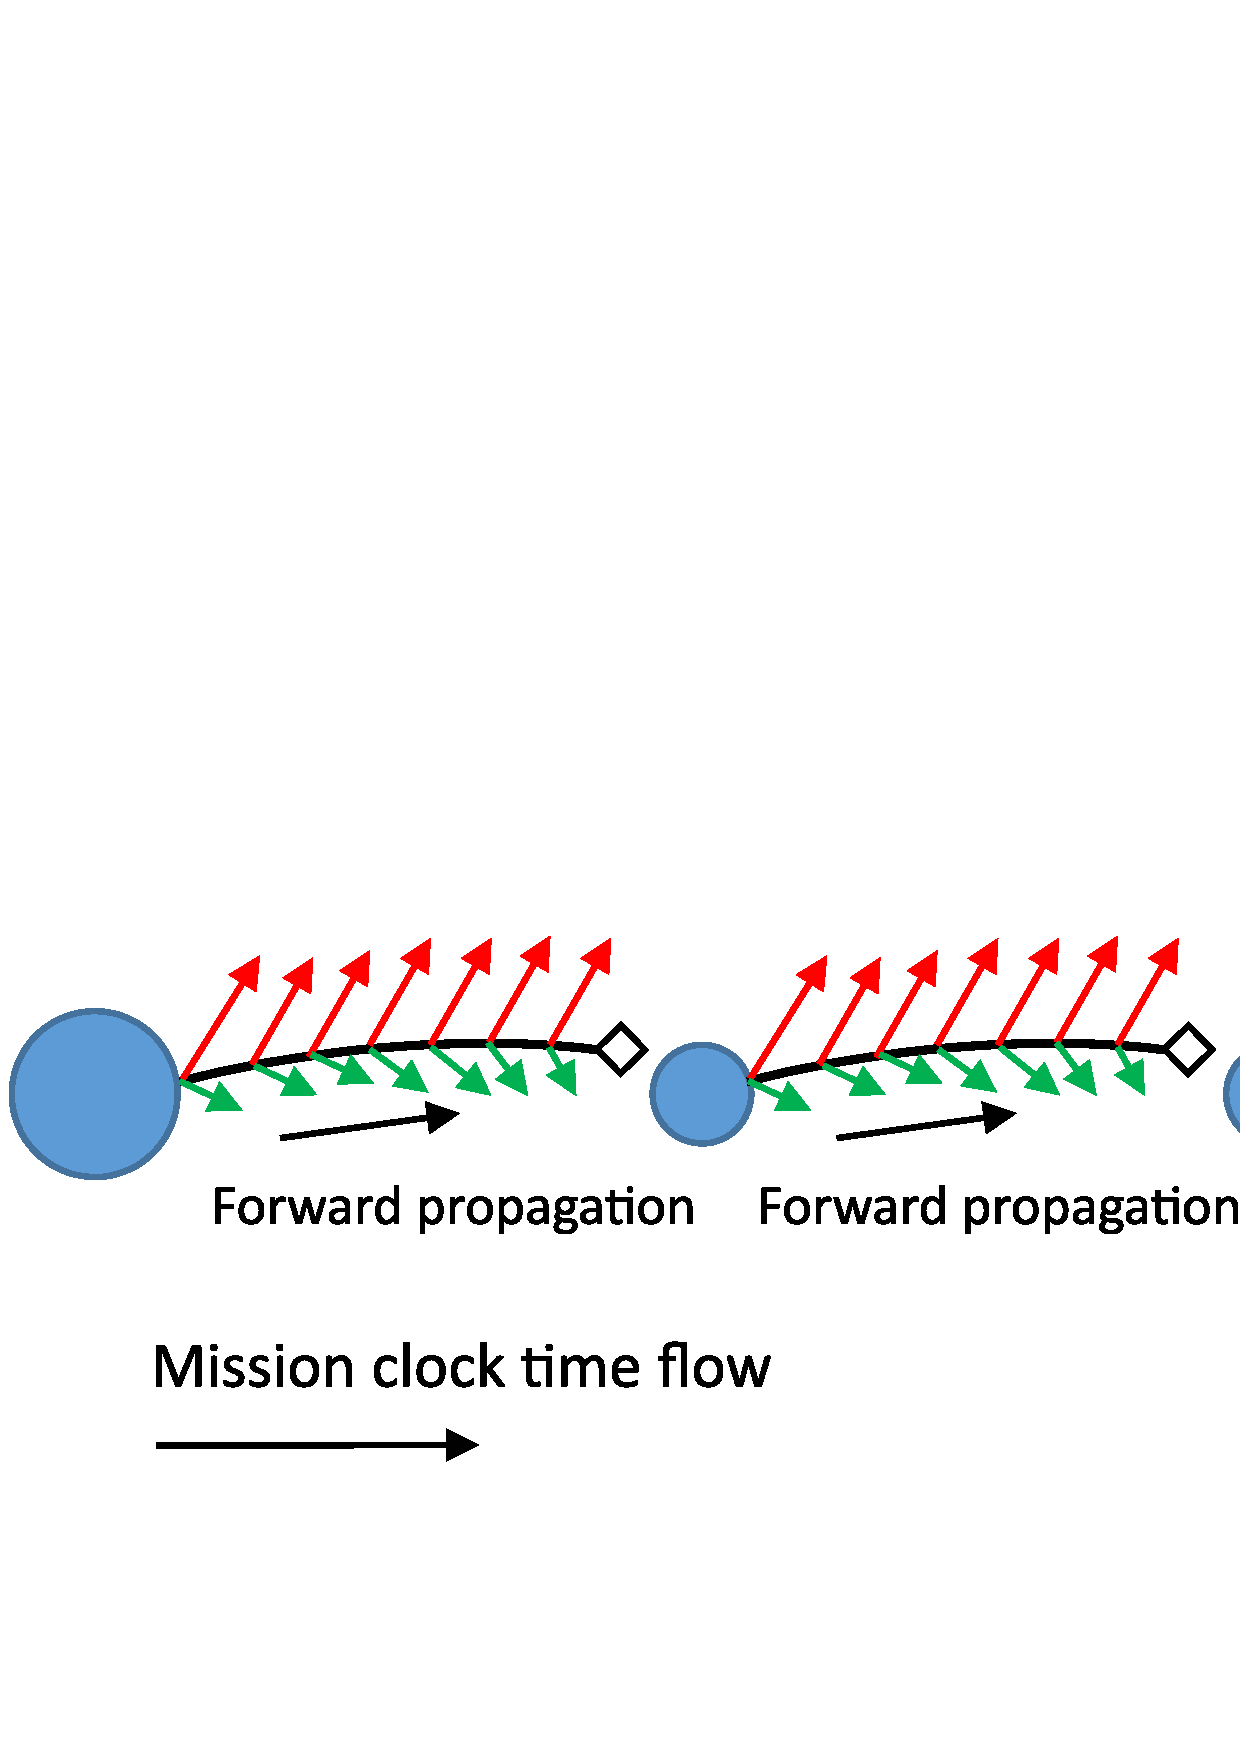
\includegraphics[width=0.9\textwidth]{../../shared_latex_inputs/images/PSFB_with_perturbations.png}
    \caption{\acf{PSFB}}
\end{figure}


\section{Parallel Shooting Bounded Impulse (PSBI)}
\label{sec:parallel_shooting_bounded_impulse}
\ac{PSBI} combines the Sims-Flanagan transcription with \ac{EMTG}'s base parallel-shooting phase classes, resulting in a low-fidelity parallel-shooting transcription. The low-thrust acceleration is modeled as a bounded impulse in the center of each time step, similar to the \ac{MGALT} transcription. Since \ac{PSBI} is a parallel-shooting method and all steps propagate forward in time, each time-step encodes the left-hand state in the decision vector and includes a set of continuity constraints to enforce equivalency between the encoded left-hand state and the previous step's propagated right-hand state. This parallel-shooting method allows for easy implementation of maneuver constraints as compared to the two-point shooting used in \ac{MGALT}. 

\begin{figure}[H]
    \centering
    \includegraphics[width=0.9\textwidth]{../../shared_latex_inputs/images/PSBI.png}
    \caption{\acf{PSBI}}
\end{figure}



\section{Probe Entry Phase}
\label{sec:probe_entry}
Probe Entry Phase is a special phase type that tracks both the trajectory of the spacecraft and that of an entry probe which separates from the spacecraft. Following separation, the probe and spacecraft are propagated separately but for the same time of flight. The entry probe propagates to some point defining atmospheric entry and then to some surface target or parachute open state. The spacecraft performs a divert maneuver to enter some desired final state, defined by the Journey arrival conditions. 

\noindent This phase type derives from the \ac{MGAnDSMs} base class and thus inherits the same departure and arrival criteria for the main spacecraft. To handle the probe, an additional arrival event is introduced to define the desired target location for the probe independent of the rest of the problem. This right-hand boundary is modeled as a Free Point Intercept, thus when using the Probe Entry Phase mission type users must set some arrival elements using the same interface as any Free Point departure or arrival class. Separation is modeled using a user-defined constant separation impulse in Newton-seconds. This impulse is applied in the direction of the probe's velocity vector at entry.  

\noindent Since Probe Entry Phase inherits from \ac{MGAnDSMs}, this is done using a two-point shooting method with a set of match points linking the forward and backward half-phases. Since the probe does not perform maneuvers after separation, the match point location is specified as a fraction of the phase time of flight, which is a user-defined constant. This allows users to force the match point to be nearer to the right-hand boundary condition, allowing small time steps to be used when the probe is near the planet. This allows some representation of atmospheric entry. The second coast subphase following the match point then includes a unique time of flight decision variable to allow the optimizer to determine the arrival event.

\noindent Since the spacecraft is propagated alongside the probe, its propagation also inherits from \ac{MGAnDSMs} and thus uses the expected two-point shooting method. The match point for the propagation of the spacecraft is attached to the divert maneuver and may be placed in any permitted location in the phase just as maneuvers are in an \ac{MGAnDSMs} phase. Effectively, the spacecraft operates as if it is a normal \ac{MGAnDSMs} phase, with an initial mass loss equal to the weight of the entry probe.

\noindent An additional constraint is enforced on the distance between the probe and the spacecraft to ensure the solution maintains a reasonably high-bandwidth communication between the entry probe and the carrier spacecraft. This constraint is applied on the state at the end of the probe's trajectory and the state at the end of the spacecraft's trajectory and is set by the user in the Journey Options via the ``Probe communication distance bounds (km)'' input.


\begin{figure}[H]
    \centering
    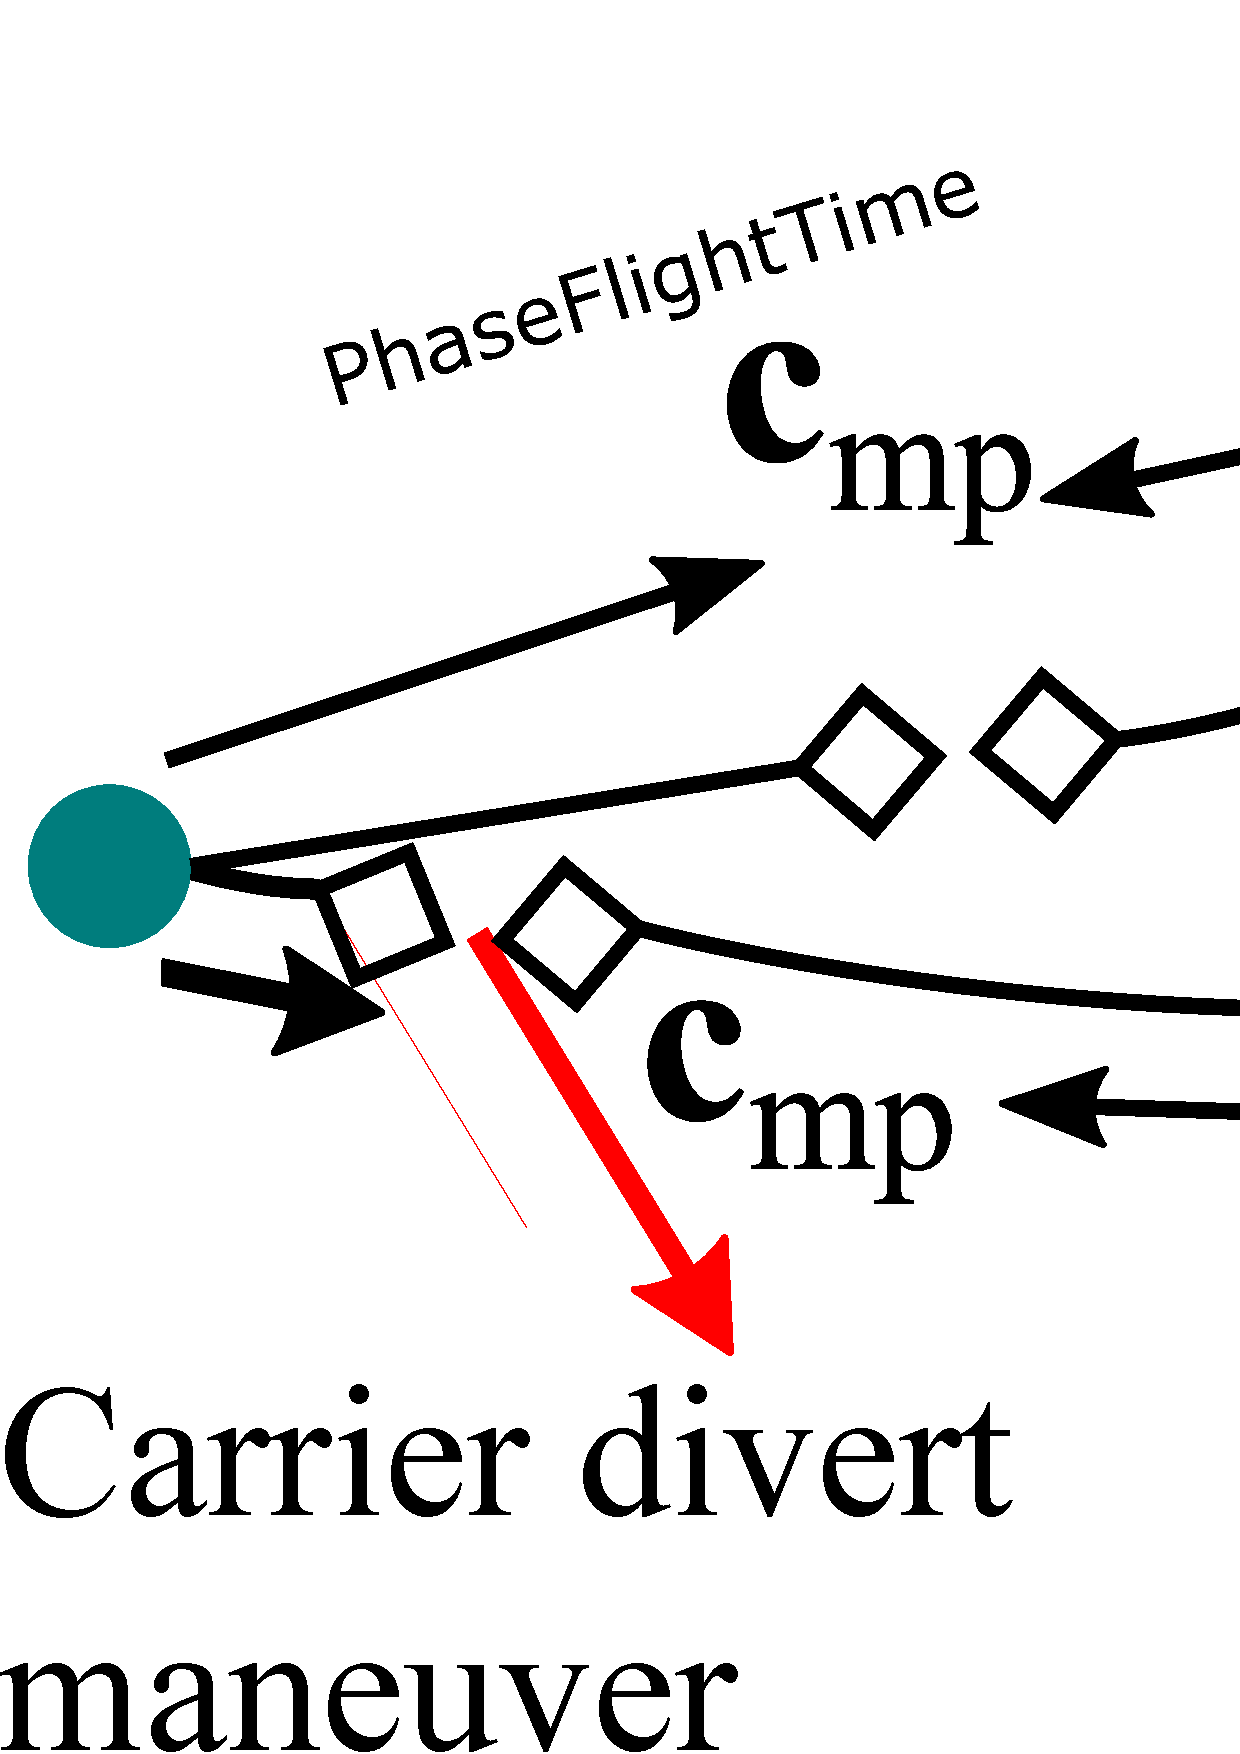
\includegraphics[width=0.9\textwidth]{../../shared_latex_inputs/images/ProbeEntryPhase_zoom.png}
    \caption{Probe Entry Phase}
\end{figure}





\chapter{Journey Boundaries}
\label{chap:journey_boundaries}
\ac{EMTG} missions consist of at least one Journey, each having a Departure and Arrival Boundary. A Boundary includes a Type (Arrival or Departure) that determines how the spacecraft arrives at or departs from the ephemeris body, and a Class that represents the spacecraft state relative to the ephemeris body. The Journey Options tab specifies the specific combination of Boundary Class and Type for each Journey's Arrival and Departure. Table \ref{tab:boundary_class_options} specifies the compatibility of the various Boundary Classes and Types.


%% nicematrix version:
\begin{table}[H]
\makebox[1 \textwidth][c]{       %centering table
\resizebox{1.1 \textwidth}{!}{   %resize table
\begin{NiceTabular}{IlIp{0.325\linewidth}Ic|c|c|cI}
    \Xhline{1.25pt}
                                                                                                        &                                                                           & \multicolumn{4}{c}{\textbf{Boundary Classes}}                                                             \\ \Xcline{3-6}{1.25pt}
                                                                                                        &                                                                           & Ephemeris-pegged          & Free Point            & Ephemeris-referenced          & Periapse              \\ 
    \Xhline{1.25pt}
    \multicolumn{1}{|l|}{\multirow{8.25}{*}{\STAB{\rotatebox[origin=c]{90}{\textbf{Departure Types}}}}} & Launch or Direct Insertion                                                & \textbf{x}                & \textbf{x}            &                               & \textbf{x}            \\ \cline{2-6} 
                                                                                                        & Depart from Parking Orbit                                                 & \textbf{x}                &                       &                               &                       \\ \cline{2-6} 
                                                                                                        & Free Direct Departure                                                     & \textbf{x}                & \textbf{x}            & \textbf{x}                    &                       \\ \cline{2-6} 
                                                                                                        & Flyby                                                                     & \textbf{x}                &                       &                               &                       \\ \cline{2-6} 
                                                                                                        & Flyby with Fixed V-Infinity out                                           &                           &                       &                               &                       \\ \cline{2-6} 
                                                                                                        & Spiral-out from Circular Orbit                                            & \textbf{x}                &                       &                               &                       \\ \cline{2-6} 
                                                                                                        & Zero Turn Flyby                                                           & \textbf{x}                &                       &                               &                       \\
    \Xhline{1.25pt}
    \multicolumn{1}{|l|}{\multirow{14}{*}{\STAB{\rotatebox[origin=c]{90}{\textbf{Arrival Types}}}}}     & \makecell[l]{Insertion into Parking Orbit \\ (use chemical Isp)}          & \textbf{x}                &                       &                               &                       \\ \cline{2-6} 
                                                                                                        & \makecell[l]{Rendezvous \\ (with chemical maneuver)}                      & \textbf{x}                & \textbf{x}            &                               &                       \\ \cline{2-6} 
                                                                                                        & Intercept with Bounded V-Infinity                                         & \textbf{x}                & \textbf{x}            & \textbf{x}                    & \textbf{x}            \\ \cline{2-6} 
                                                                                                        & \makecell[l]{Rendezvous \\ (no maneuver)}                                 & \textbf{x}                & \textbf{x}            & \textbf{x}                    &                       \\ \cline{2-6} 
                                                                                                        & \makecell[l]{Match Final V-Infinity Vector \\ (with chemical maneuver)}   &                           &                       &                               &                       \\ \cline{2-6} 
                                                                                                        & \makecell[l]{Match Final V-Infinity Vector \\ (no maneuver)}              &                           &                       &                               &                       \\ \cline{2-6} 
                                                                                                        & Capture Spiral                                                            & \textbf{x}                &                       &                               &                       \\ \cline{2-6} 
                                                                                                        & Momentum Transfer                                                         & \textbf{x}                &                       &                               &                       \\  
    \Xhline{1.25pt}
\end{NiceTabular}
} %close resize
} %close centering
\caption{Boundary Class and Type Compatibility}
\label{tab:boundary_class_options}
\end{table}     
                                                                                                                                                                                           


\section{Boundary Classes}
\label{sec:boundary_class}

    \subsection{Ephemeris-pegged}
    \label{sec:ephem_pegged}
    The Ephemeris-pegged Boundary Class represents a boundary at the center of an ephemeris body such as the center of mass of a planet. Typically this Boundary Class is only useful for initial mission design such as patched-conic models of planetary flybys. The ``ephemeris source'' setting on the Physics Options tab controls how \ac{EMTG} determines the location of the ephemeris body. See Section \ref{sec:physics_options}.

    \subsection{Ephemeris-referenced}
    \label{sec:ephem_referenced}
    The Ephemeris-referenced Boundary Class defined relative to an ephemeris point but not on the ephemeris point. In other words, the boundary point is ``referenced'' to an ephemeris point and moves with it, but additional information is needed to define the boundary relative to the ephemeris point. In \ac{EMTG}, Ephemeris-referenced boundary conditions are defined as lying on a triaxial ellipsoid centered on an ephemeris point. For example, this could be the surface of the sphere of influence of a planet or a triaxial ellipsoid representing the surface of a non-spherical body like Ceres. The user provides the three semi-axes of the ellipsoid in the \ac{ICRF} where the center of the ellipsoid is the ephemeris body.

    \subsection{Free Point}
    \label{sec:free_point}
    The Free Point Boundary Class represents a point in space that is defined as a cartesian, orbit element, spherical, or b-plane state relative to the central body. The user may choose to fix or vary within bounds any of the six elements of the position and velocity state on the left-hand side of the boundary. 

    \subsection{Periapse}
    \label{sec:periapse_boundary}
    The Periapse Boundary Class represents events that happen at periapse of the spacecraft's orbit about the central body. In the current implementation, this class only guarantees that the spacecraft be at an apse, not necessarily the right one. Note that if a state representation that includes true anomaly (\ac{COE}, IncomingBplane, or OutgoingBplane) is chosen, then a periapse is guaranteed.

\section{Departure Types}
\label{sec:departure_boundaries}

    \subsection{Launch or Direct Insertion}
    \label{sec:launch_or_direct_insertion} 
    This Departure Type models launch from a body or an impulsive departure using three decision variables, the magnitude of the departure $v_{\infty}$, and the right ascension and declination of the departure asymptote in the \ac{ICRF}. 

    \subsection{Depart from Parking Orbit}
    \label{sec:depart_from_park_orbit} 
    Depart from a parking orbit around the departure body. Use a Free Point Boundary Class to specify parameters of the orbit. 

    \subsection{Free Direct Departure}
    \label{sec:free_direct_departure}
    Free Direct Departure is a type of boundary event in which a spacecraft departs from a point in space that is defined as a cartesian or \ac{COE} state relative to the central body. The user may choose to fix any of the state elements relative to the central body or allow them to vary within specified bounds on the left-hand side of the boundary. 

    \subsection{Flyby}
    \label{sec:flyby}
    A flyby is a trajectory segment in which a spacecraft passes close to a celestial body and uses the body's gravity to alter its trajectory. In \ac{EMTG}, flybys are modeled using patched-conic approximations, which divide the trajectory into segments based on the gravitational influence of each celestial body. The spacecraft's trajectory is approximated as a series of conic sections that are tangent at the points where they transition from one body's sphere of influence to another. At later phases of mission design, flybys are modeled at higher fidelity using other Boundary Event combinations to go from incoming \ac{SOI} crossing to periapse to outgoing \ac{SOI} crossing.

    \subsection{Flyby with Fixed V-Infinity Out}
    \label{sec:flyby_fixed_vinf_out}
    Flyby with Fixed V-Infinity Out is a type of outgoing flyby used when the user wants to specify the value of $v_{\infty-out}$. This boundary event includes two equality constraints to guarantee that the magnitude and direction of $v_{\infty-out}$ match the user-specified values.

    \subsection{Zero Turn Flyby}
    \label{sec:zero_turn_flyby}
    This Departure Type is used when the flyby is of a very small body and therefore the change in the direction of the spacecraft velocity due to the body is small enough to not be modeled. When zero turn flyby and ephemeris point are used together, \ac{EMTG} enforces the constraint that the spacecraft  $v_{\infty-out}$ matches $v_{\infty-in}$. Users must take care that the small body assumption is sufficient, as this will ignore any velocity change that would normally occur even if a larger planetary body is chosen as the start location for the journey.


    \subsection{Spiral-out from Circular Orbit}
    \label{sec:spiral_out}
    Spiral-out from circular orbit is a technique used in \ac{EMTG} to approximate a many-revolution low-thrust spiral about a body in the current universe. For example, one may wish to spiral from \ac{LEO} to escape from the Earth, or from the edge of the Mars sphere of influence down to the orbital distance of Phobos or Deimos. Edelbaum's approximation provides a fast, sufficiently accurate model that allows spirals to be included with an \ac{EMTG} broad search without having to explicitly model and optimize the path of the spacecraft during the spiral. Edelbaum's approximation consists of modeling the initial and final orbits about the body as co-planar circles and then assuming that the thrust level is sufficiently low that the transfer orbit is also nearly circular.


\section{Arrival Types}
\label{sec:arrival_boundaries}

    \subsection{Insertion into Parking Orbit (use chemical Isp)}
    \label{sec:insert_parking_orbit} 
    Specifies that \ac{EMTG} should solve for a maneuver that places the spacecraft into a parking orbit using its chemical thruster upon arrival at this body. Depending on the Boundary Class selected, users may specify only the \ac{SMA} and \ac{ECC} of the parking orbit (Ephemeris-pegged Class) or a full set of varying or specified state variables (Free Point Class). 

    \subsection{Rendezvous (with chemical maneuver)}
    \label{sec:rendezvous_arrival}
    This arrival type specifies that the spacecraft perform a chemical maneuver upon reaching the arrival body to either match velocities with the body in the case of an Ephemeris-pegged Boundary Class or achieve a state relative to the ephemeris body when combined with another Boundary Class.

    \subsection{Intercept with Bounded V-Infinity}
    \label{sec:intercept_bounded_vinfty}
    This arrival type specifies that the spacecraft arrive at the ephemeris body with some maximum magnitude of velocity at infinity, $v_{\infty}$, given by 

        \begin{align}
            v_{\infty} &= \sqrt{v^2 - \frac{2 \mu}{r}}.
        \end{align}

    \subsection{Rendezvous (no maneuver)}
    \label{sec:rendezvous_no_maneuver}
    This arrival type specifies that the spacecraft matches position and velocity with some point upon arrival. This point may be defined as some ephemeris point in the case of an Ephemeris-pegged Boundary Class, some point on the edge of the ephemeris bounding ellipse in the case of an Ephemeris-referenced Boundary Class, or some user defined Free Point in the case of the Free Point Boundary Class. This is generally intended for use explicitly with low-thrust transcriptions.

    \subsection{Match Final V-Infinity Vector (with chemical maneuver)}
    \label{sec:mathc_final_vinfty_vec_chemical_maneuver}
    Arrival Type that forces the spacecraft to match a specified $v_{\infty}$ vector upon arrival using a chemical maneuver. Selecting this Arrival Type in the Journey Options tab reveals additional options to specify the $v_{\infty}$ vector. % #?? is this in \ac{ICRF}?

    \subsection{Match Final V-Infinity Vector (no maneuver)}
    \label{sec:mathc_final_vinfty_vec_no_maneuver}
    Arrival Type that forces the spacecraft to match a specified $v_{\infty}$ vector upon arrival using a chemical maneuver. Selecting this Arrival Type in the Journey Options tab reveals additional options to specify the $v_{\infty}$ vector. % #?? is this in \ac{ICRF}?

    \subsection{Capture Spiral}
    \label{sec:capture_spiral}
    Models a many-revolution low-thrust spiral capture about a body in the current universe similarly to the ``spiral-out from circular orbit'' Departure Type

    \subsection{Momentum Transfer}
    \label{sec:momentum_transfer}
    Momentum Transfer is a specific type of Arrival Type used in unique scenarios where the spacecraft collides with the destination body, resulting in the transfer of momentum to the body.




\chapter{Universe File and Options}
\label{chap:universe_options}

\ac{EMTG} Universe files define all celestial body and ephemeris data required by \ac{EMTG}. This mostly consists of astrodynamics data pertaining to the central body. For a given Journey, the geometric center of the central body serves as the center of propagation in \ac{EMTG}. The file takes the extension {\tt .emtg\_universe} and consists of two major sections: the central body information and a menu of bodies which define the list of available flyby objects for the Journey. 

\section{Central Body Definition}
The central body information is used to define the central body for a given Journey, and thus multiple {\tt .emtg\_universe} files are required when multiple central bodies are needed in a mission. This information is listed first in an {\tt .emtg\_universe} file but is not contained in any specific block. The lines and expected data types are shown in Table \ref{tab:universe_centralbodyinfo}, with additional details following.

\begin{table}[H]
    \centering
    % \begin{tabular}{l|l|l}
    \begin{tabular}{llll}
    \hline
    \textbf{Line} & \textbf{Line Name} & \textbf{Data Type} \\
    \hline
    \textbf{1} & central\_body\_name & String \\
    % \hline
    \textbf{2} & central\_body\_SPICE\_ID & Integer \\
    % \hline
    \textbf{3} & central\_body\_radius & Real (km) \\
    % \hline
    \textbf{4} & central\_body\_J2 & Real \\
    % \hline
    \textbf{5} & central\_body\_J2\_reference\_radius & Real (km) \\
    % \hline
    \textbf{6} & central\_body\_flattening\_coefficient & Real \\
    % \hline
    \textbf{7} & mu & Real (km\textsuperscript{3}/s\textsuperscript{2}) \\
    % \hline
    \textbf{8} & LU & Real (km) \\
    % \hline
    \textbf{9} & reference\_angles & Real (degrees) \\
    % \hline
    \textbf{10} & r\_SOI & Real (km) \\
    % \hline
    \textbf{11} & minimum\_safe\_distance & Real (km)
    \end{tabular}
    \caption{Universe File Central Body Information}
    \label{tab:universe_centralbodyinfo}
\end{table}


\noindent\listitem{central\_body\_name}{The name of the central body.}
\listitem{central\_body\_SPICE\_ID}{The \ac{SPICE} ID associated with the central body.}
\listitem{central\_body\_radius}{The radius of the central body.}
\listitem{central\_body\_J2}{Optionally provided J2 value for the central body. Defaults to 0.}
\listitem{central\_body\_J2\_reference\_radius}{Optionally provided J2 reference radius for the central body. Defaults to 0.}
\listitem{central\_body\_flattening\_coefficient}{Optionally provided flattening coefficient to define oblateness of central body. Defaults to 0.}
\listitem{mu}{Gravitational constant of central body.}
\listitem{LU}{The characteristic length unit used in scaling the problem internally.}
\listitem{reference\_angles}{Six space-delimited values: alpha0, alphadot, delta0, deltadot, W, Wdot. These angles define the local reference frame relative to \ac{ICRF}, in degrees and degrees per century. The angle alpha0 defines the right ascension angle used to describe the north pole of the central body relative to the invariable plane of the solar system. The angle delta0 defines the declination angle describing the angular distance of the central body's north pole from the celestial equator. The angle W defines the location of the prime meridian of the central body measured easterly along the body's equator from a node defined as an intersection of the body equator with the celestial equator. The angular rates alphadot, deltadot, and Wdot are the rates of change of the associated angles due to precession of the axis of rotation.}
\listitem{r\_SOI}{Radius of the central body's sphere of influence.}
\listitem{minimum\_safe\_distance}{The minimum safe distance from the central body, some value greater than the radius of the central body.}





\section{Menu of Bodies Details}
The menu of bodies details information similar to that of the central body, but instead for a list of bodies available for flybys or third body perturbation effects. The menu of bodies is attached to the {\tt .emtg\_universe} file much the same way as a central body, so for missions where multiple central bodies are used the menu of bodies must be present in each {\tt .emtg\_universe} file. Unlike the central body information however, each body has all of its information listed on one space delimited line. The indices, varibale names, and expected data types are shown in Table \ref{tab:universe_menuofbodiesinfo}, with additional details following.


\begin{table}[H]
    \centering
    \begin{tabular}{lll}
    \hline
    \textbf{Index} & \textbf{Variable Name} & \textbf{Data Type} \\
    \hline
    \textbf{1} & Name & String \\
    % \hline
    \textbf{2} & Short Name & String \\
    % \hline
    \textbf{3} & Number & Integer \\
    % \hline
    \textbf{4} & \ac{SPICE}\_ID & Integer \\
    % \hline
    \textbf{5} & minimum\_flyby\_altitude & Real (km) \\
    % \hline
    \textbf{6} & GM & Real (km\textsuperscript{3}/s\textsuperscript{2}) \\
    % \hline
    \textbf{7} & Radius & Real (km) \\
    % \hline
    \textbf{8} & body\_flattening\_coefficient  & Real \\
    % \hline
    \textbf{9} & body\_J2 & Real \\
    % \hline
    \textbf{10} & body\_AbsoluteMagnitude & Real \\
    % \hline
    \textbf{11} & body\_albedo & Real \\
    % \hline
    \textbf{12} & ephemeris\_epoch & Real \\
    % \hline
    \textbf{13} & alpha0 & Real (degrees) \\
    % \hline
    \textbf{14} & alphadot & Real (degrees/century) \\
    % \hline
    \textbf{15} & delta0 & Real (degrees) \\
    % \hline
    \textbf{16} & deltadot & Real (degrees/century) \\
    % \hline
    \textbf{17} & W & Real (degrees) \\
    % \hline
    \textbf{18} & Wdot & Real (degrees/century) \\
    % \hline
    \textbf{19} & \acs{SMA} & Real (km) \\
    % \hline
    \textbf{20} & \acs{ECC} & Real \\
    % \hline
    \textbf{21} & \acs{INC} & Real (degrees) \\
    % \hline
    \textbf{22} & \acs{RAAN} & Real (degrees) \\
    % \hline
    \textbf{23} & \acs{AOP} & Real (degrees) \\
    % \hline
    \textbf{24} & \acs{MA} & Real (degrees) \\
    % \hline
    \end{tabular}
    \caption{Universe File Menu Of Bodies Specifications}
    \label{tab:universe_menuofbodiesinfo}
\end{table}


\noindent\listitem{Name}{Details a full name for a body appearing on the menu of bodies.}
\listitem{Short Name}{A short hand call out to a body which is used to name results files. Often a single letter (e.g., J for Jupiter).}
\listitem{Number}{A number associated with the body, used to set destination lists and flyby sequences as an easy to parse list of integers.}
\listitem{\ac{SPICE}\_ID}{The \ac{SPICE} ID associated with the body being set. Lists of IDs are available at \href{https://naif.jpl.nasa.gov/pub/naif/toolkit_docs/C/req/naif_ids.html}{https://naif.jpl.nasa.gov/pub/naif/toolkit\_docs/C/req/naif\_ids.html}.}
\listitem{minimum\_flyby\_altitude}{A lower bound on the safe flyby altitude for a body appearing on the list of available flyby objects. If the value is $\leq 0$, the object is not placed on the flyby menu.}
\listitem{GM}{The gravitational parameter of the body.}
\listitem{Radius}{The radius of the body.}
\listitem{body\_flattening\_coefficient}{A flattening coefficient defining the oblateness of the body.}
\listitem{body\_J2}{The J2 zonal harmonic term of the body.}
\listitem{body\_AbsoluteMagnitude}{The brightness of the body. This is included for future use in a genetic algorithm to aid in defining a potentially interesting small body flyby.}
\listitem{body\_albedo}{The fraction of light a body reflects. This is used with the body absolute magnitude to estimate the body radius.}
\listitem{ephemeris\_epoch}{A reference epoch for the body provided as a modified Julian date, used to verify the body exists in the provided \ac{SPICE} ephemeris at this point.}
\listitem{alpha0}{The right ascension angle used to define the pole of rotation that lies on the north side of the invariable plane of the solar system. This right ascension describes the angular distance from the Earth equinox at J2000 and the hour circle passing through the object, the hour circle being the great circle passing through a celestial object and the two celestial poles.}
\listitem{alphadot}{The rate of change of the right ascension angle used to define the pole of rotation of the celestial body due to precession of the axis of rotation of the body.}
\listitem{delta0}{The declination angle used to define the pole of rotation that lies on the north side of the invariable plane of the solar system. This declination describes the angular distance of said north pole to the celestial (\ac{ICRF}) equator.}
\listitem{deltadot}{The rate of change of the declination angle used to define the pole of rotation of the celestial body due to precession of the axis of rotation of the body}
\listitem{W}{The angle defining the location of the prime meridian of the celestial body, measured easterly along the body's equator from a node defined as an intersection of the body equator with the celestial (\ac{ICRF}) equator.}
\listitem{Wdot}{The rate of change of the angle used to define the location of the prime meridian of the celestial body due to precession of the axis of rotation of the body}
\listitem{SMA}{Semi-major axis of the body at the provided reference epoch with respect to the central body local reference frame. Overridden if ephemeris is drawn from \ac{SPICE}.}
\listitem{ECC}{Eccentricity of the body at the provided reference epoch with respect to the central body local reference frame. Overridden if ephemeris is drawn from \ac{SPICE}.}
\listitem{INC}{Inclination of the body at the provided reference epoch with respect to the central body local reference frame. Overridden if ephemeris is drawn from \ac{SPICE}.}
\listitem{RAAN}{Right Ascension of the Ascending Node of the body at the provided reference epoch with respect to the central body local reference frame. Overridden if ephemeris is drawn from \ac{SPICE}.}
\listitem{AOP}{Argument of Perigee of the body at the provided reference epoch with respect to the central body local reference frame. Overridden if ephemeris is drawn from \ac{SPICE}.}
\listitem{MA}{Mean Anomaly of the body at the provided reference epoch with respect to the central body local reference frame. Overridden if ephemeris is drawn from \ac{SPICE}.}

\chapter{EMTG Options}
\label{chap:options}
An \ac{EMTG} mission is created through a text file known as an \ac{EMTG} Options file with the extension \verb|.emtgopt|. \ac{EMTG} Options files define the mission parameters as well as link to the ephemeris and hardware configuration needed for the mission. The ephemeris configuration is another text file known as an \ac{EMTG} Universe file with extension \verb|.emtg_universe|. Hardware configurations are stored in another set of text files for the launch vehicle and spacecraft with extensions \verb|.emtg_launchvehicleopt| and \verb|.emtg_spacecraftopt|. \ac{EMTG} Options files can be configured using a text editor or the PyEMTG \ac{GUI}. This chapter will discuss the \ac{EMTG} Options file and PyEMTG interface.

\noindent Most interaction with the \ac{EMTG} Options file can be accomplished through PyEMTG though some options are only present in the \verb|.emtgopt| file and must be changed there using a text editor. An \ac{EMTG} Options file can be created in PyEMTG by selecting "File, New, Mission" (Ctrl + m). An existing \ac{EMTG} Options file can be opened by selecting "File, Open" (Ctrl + o) and choosing an existing \verb|.emtgopt| file.

\begin{figure}[H]
    \centering
    \includegraphics[width=0.5\textwidth]{../../shared_latex_inputs/images/pyemtg_file_new.png}
    \caption{Creating a new EMTG Options file}
\end{figure}

\noindent An \ac{EMTG} Options file is broken up into several sections shown with tabs in PyEMTG: Global Mission Options, Spacecraft Options, Journey Options, Solver Options, Physics Options, and Output Options. The rest of the chapter will cover each of the sections in turn as well as the options that can only be accessed through the \verb|.emtgopt| text file.

\begin{figure}[H]
    \centering
    \includegraphics[width=0.9\textwidth]{../../shared_latex_inputs/images/pyemtg_options_tabs.png}
    \caption{EMTG Options tabs}
\end{figure}

	
\section{Global Mission Options and Constraints}
\label{sec:global_options}
The Global Mission Options tab covers options and constraints that apply to the entire mission such as the objective function, launch bounds, overall mission time bounds, and other settings.


\begin{figure}[H]
    \centering
    \includegraphics[width=1.0\textwidth]{../../shared_latex_inputs/images/pyemtg_global_options_tab.png}
    \caption{EMTG Global Options tab}
\end{figure}

\subsection{Global Mission Options}

\begin{enumerate}

    \item \textbf{Mission Name:} The mission name is used to distinguish \ac{EMTG} missions and will prefix the output directories and files \ac{EMTG} produces when a mission is run.

        \begin{table}[H]
            \hspace{2cm}
            \begin{tabular}{ll}
            Data Type & \verb|string| \\
            Default Value & ``default'' \\
            \end{tabular}
        \end{table}

    \item \textbf{Mission Type:} \ac{EMTG} provides several different Mission Types which control how an \ac{EMTG} mission is modeled. Mission Types come in various levels of fidelity and may be selected for the entire mission or on a per-Journey basis. Mission Types are covered in more detail in Chapter~\ref{chap:mission_types}.
        \begin{table}[H]
            \hspace{2cm}
            \begin{tabular}{lp{3cm}}
            Data Type & \verb|PhaseType| \\
            Allowed Values & \verb|MGALT, FBLT, PSBI, PSFB, MGAnDSMs, CoastPhase,| \newline
                             \verb|SundmanCoastPhase, Variable phase type,| \newline
                             \verb|ProbeEntryPhase, ControlLawThrustPhase| \\
            Default Value & \verb|MGALT| \\
            \end{tabular}
        \end{table}

    \item \textbf{Objective Function:} This option specifies the mission parameter to be maximized or minimized such as maximizing final mass or minimizing delta-v.
    
        \begin{table}[H]
            \hspace{2cm}
            \begin{tabular}{lp{5cm}}
            Data Type & \verb|PhaseType| \\
            Allowed Values & \verb|0: minimum deterministic deltaV,| \newline
                             \verb|1: minimum time,| \newline
                             \verb|2: maximum final mass,| \newline
                             \verb|3: maximize initial mass,| \newline
                             \verb|4: depart as late as possible,| \newline
                             \verb|5: depart as early as possible,| \newline
                             \verb|6: maximize orbit energy,| \newline
                             \verb|7: minimize launch mass,| \newline
                             \verb|8: arrive as early as possible,| \newline
                             \verb|9: arrive as late as possible,| \newline
                             \verb|10: minimum propellant,| \newline
                             \verb|11: maximum dry/wet ratio,| \newline
                             \verb|12: maximum arrival kinetic energy,| \newline
                             \verb|13: minimum BOL power,| \newline
                             \verb|14: maximize log\_10(final mass),| \newline
                             \verb|15: maximize log\_e(final mass),| \newline
                             \verb|16: maximum dry mass margin,| \newline
                             \verb|17: maximum dry mass,| \newline
                             \verb|18: maximum log\_10(dry mass),| \newline
                             \verb|19: maximum log\_e(dry mass),| \newline
                             \verb|20: minimize chemical fuel,| \newline
                             \verb|21: minimize chemical oxidizer,| \newline
                             \verb|22: minimize electric propellant,| \newline
                             \verb|23: minimize total propellant,| \newline
                             \verb|24: minimize waypoint tracking error,| \newline
                             \verb|25: minimize initial impulse magnitude,| \newline
                             \verb|26: maximize distance from central body| \\
            Default Value & \verb|2: maximum final mass| \\
            \end{tabular}
        \end{table}

    \item \textbf{Include initial impulse in total deterministic delta-v:} This options controls whether or not the delta-v provided by the launch vehicle is included in the objective function, ``0: minimum deterministic deltaV.''
        
        \begin{table}[H]
            \hspace{2cm}
            \begin{tabular}{ll}
            Data Type & \verb|bool| \\
            Allowed Values & true, false \\
            Default Value & false \\
            Units & NA
            \end{tabular}
        \end{table}

    \item \textbf{Launch window open date:} The earliest possible launch date expressed as an MJD2000 value. This value can be set using the text box or the calendar tool below.
    
        \begin{table}[H]
            \hspace{2cm}
            \begin{tabular}{ll}
            Data Type & \verb|double| \\
            Allowed Values & 0 $<$ Real $<$ $\infty$ \\
            Default Value & 0.0 \\
            Units & days since MJD2000 epoch
            \end{tabular}
        \end{table}
    
    \item \textbf{Number of time-steps:} Number of time-steps per journey/phase. This controls how many segments define each Journey. A higher value increases the mission fidelity at the cost of run time. This option can be overridden on a per-Journey basis in the Journey Options tab.
    
        \begin{table}[H]
            \hspace{2cm}
            \begin{tabular}{ll}
            Data Type & \verb|int| \\
            Allowed Values & 0 $<$ Integer $<$ $\infty$ \\
            Default Value & 20 \\
            Units & NA
            \end{tabular}
        \end{table}
        
    \item \textbf{Stop after journey (indexed from 0):} This will cause \ac{EMTG} to only optimize up to and including the integer Journey number set in the text box. For example, if the \ac{EMTG} Options file has 3 Journeys (Journey 0 to Journey 2) and this text box is set to 1, \ac{EMTG} will not solve Journey 2.

        \begin{table}[H]
            \hspace{2cm}
            \begin{tabular}{ll}
            Data Type & \verb|int| \\
            Allowed Values & 0 $<$ Integer $<$ (Number of Journeys - 1) \\
            Default Value & 32767 \\
            Units & NA
            \end{tabular}
        \end{table}
    

\end{enumerate}
    
\subsection{Global Mission Constraints}

\begin{enumerate}
    \item \textbf{RLA bounds (degrees):} Bound the right ascension of the launch asymptote (equatorial east longitude from the vernal equinox).

        \begin{table}[H]
            \hspace{2cm}
            \begin{tabular}{ll}
            Data Type & \verb|std::vector<double, 2>| \\
            Allowed Values & -$\infty$ $<$ Real $<$ $\infty$ \\
            Default Value & [-2880.0, 2880.0] \\
            Units & degrees
            \end{tabular}
        \end{table}

    \item \textbf{\acs{DLA} bounds (degrees):} Bound the declination (latitude) of the launch asymptote. 
    
        \begin{table}[H]
            \hspace{2cm}
            \begin{tabular}{ll}
            Data Type & \verb|std::vector<double, 2>| \\
            Allowed Values & -90 $<$ Real $<$ 90 \\
            Default Value & [-90.0, 90.0] \\
            Units & degrees
            \end{tabular}
        \end{table}

    \item \textbf{Enable mission time bounds:} Selecting this box will reveal the Global flight time upper and lower bounds boxes to constrain the mission length.
    
        \begin{table}[H]
            \hspace{2cm}
            \begin{tabular}{ll}
            Data Type & \verb|bool| \\
            Allowed Values & true, false \\
            Default Value & true \\
            Units & NA
            \end{tabular}
        \end{table}

    \item \textbf{Global flight time bounds (days):} Used to set boundaries on mission length in days where 0.0 is the launch epoch. Revealed and active only if "Enable mission time bounds" is checked.
    
        \begin{table}[H]
            \hspace{2cm}
            \begin{tabular}{ll}
            Data Type & \verb|std::vector<double, 2>| \\
            Allowed Values & 0 $<$ Real $<$ $\infty$ \\
            Default Value & [0, 302] \\
            Units & days
            \end{tabular}
        \end{table}

    \item \textbf{Forced post-launch coast duration (days):} Restrict \ac{EMTG} from placing any maneuvers between launch and this option's value in days. This can be used to ensure adequate time for spacecraft checkout after launch.
    
        \begin{table}[H]
            \hspace{2cm}
            \begin{tabular}{ll}
            Data Type & \verb|double| \\
            Allowed Values & 0 $<$ Real $<$ $\infty$ \\
            Default Value & 0.0 \\
            Units & days
            \end{tabular}
        \end{table}

    \item \textbf{Forced pre-flyby coast duration (days):} Restrict \ac{EMTG} from placing any maneuvers this many days prior to a planetary flyby. This can be used to ensure adequate time for trajectory error cleanup prior to the flyby.
    
        \begin{table}[H]
            \hspace{2cm}
            \begin{tabular}{ll}
            Data Type & \verb|double| \\
            Allowed Values & 0 $<$ Real $<$ $\infty$ \\
            Default Value & 0.0 \\
            Units & days
            \end{tabular}
        \end{table}

    \item \textbf{Forced post-flyby coast duration (days):} Restrict \ac{EMTG} from placing any maneuvers this many days after a planetary flyby.
    
        \begin{table}[H]
            \hspace{2cm}
            \begin{tabular}{ll}
            Data Type & \verb|double| \\
            Allowed Values & 0 $<$ Real $<$ $\infty$ \\
            Default Value & 0.0 \\
            Units & days
            \end{tabular}
        \end{table}

    \item \textbf{Magnitude of post-launch TCM (km/s):} Sets the upper bound on a post-launch TCM. \ac{EMTG} sets the lower bound to 0 km/s internally. The post-launch TCM is assumed to be performed by the monopropellant propulsion system and is used to compute the mass loss due to the TCM on the left boundary of a phase.
    
        \begin{table}[H]
            \hspace{2cm}
            \begin{tabular}{ll}
            Data Type & \verb|double| \\
            Allowed Values & 0 $<$ Real $<$ $\infty$ \\
            Default Value & 0.0 \\
            Units & km/s
            \end{tabular}
        \end{table}

    \item \textbf{Magnitude of pre-flyby TCM (km/s):} Sets the upper bound on a pre-flyby TCM. \ac{EMTG} sets the lower bound to 0 km/s internally. The pre-flyby TCM is assumed to be performed by the monopropellant propulson system and is used to compute the mass loss due to TCM immediately before a flyby.

        \begin{table}[H]
            \hspace{2cm}
            \begin{tabular}{ll}
            Data Type & \verb|double| \\
            Allowed Values & 0 $<$ Real $<$ $\infty$ \\
            Default Value & 0.0 \\
            Units & km/s
            \end{tabular}
        \end{table}

    \item \textbf{Constrain final/dry mass?:} Checking either of these options reveals a set of text boxes to bound either the final mass or the dry mass of the spacecraft at the end of the mission. Final mass is also known as final wet (including propellant) mass. These options are applied separately, allowing users to constrain both the vehicle dry mass and the final mission mass at the same time. 

        \begin{table}[H]
            \hspace{2cm}
            \begin{tabular}{ll}
            Data Type & bool \\
            Allowed Values & true, false \\
            Default Value & false \\
            Units & NA
            \end{tabular}
        \end{table}

    \item \textbf{Final/dry mass constraint value (kg):} Mass values for the final/dry mass constraint. Revealed and active only if either the constrain final or dry mass is active.
    
        \begin{table}[H]
            \hspace{2cm}
            \begin{tabular}{ll}
            Data Type & \verb|std::vector<double, 2>| \\
            Allowed Values & 0 $<$ Real $<$ $\infty$ \\
            Default Value & [0.0, 0.0] \\
            Units & kg
            \end{tabular}
        \end{table}

\end{enumerate}

	\section{Spacecraft Options}
\label{sec:spacecraft_options}

The Spacecraft Options tab allows users to specify the launch vehicle and spacecraft used to define a mission. The launch vehicle is defined explicitly with a configuration file, while a spacecraft may be defined either via configuration files or within the Spacecraft Options tab directly. The spacecraft configuration files allow for greater flexibility when defining a spacecraft than may be easily achieved via the PyEMTG window. For details on how to create configuration files for launch vehicles and spacecraft, as well as the available propulsion, power, and constraint options which may be defined, refer to Chapter \ref{chap:config_files}.

\noindent While many of the options defining spacecraft are explicitly defined in the configuration files, some of the options defining how \ac{EMTG} handles a spacecraft still must be set in the Spacecraft Options tab.

\subsection{Common Hardware Options}
Common hardware options define the most general parameters for a missions vehicles as well as the spacecraft model type used to define the spacecraft.


\begin{enumerate}
    \item \textbf{Maximum mass (kg):} A ``maximum mass'' field which scales the optimization problem. In \ac{EMTG}, the actual launch mass is limited to whatever the launch vehicle can carry to the C3 chosen by the optimizer. The launch vehicle configuration file contains settings which define the function relating injected mass to C3 (see Section \ref{sec:lv_config}).
    \begin{table}[H]
        \hspace{2cm}
        \begin{tabular}{lp{5cm}}
        \ac{EMTG} Variable Name & \verb|maximum_mass| \\
        Data Type & \verb|double| \\
        Allowed Values & 1.0E-10 $<$ Real $<$ 1.0E-30 \\
        Default Value & $525.2$ \\
        Units & kg
        \end{tabular}
    \end{table}
    
    \item \textbf{Allow initial mass to vary:} Option to allow \ac{EMTG} to use less initial mass than the launch vehicle can inject to a given C3 if that results in a higher final mass. Initial mass is still bounded by the capabilities of the launch vehicle (i.e., injected mass to C3).
    \begin{table}[H]
        \hspace{2cm}
        \begin{tabular}{lp{5cm}}
        \ac{EMTG} Variable Name & \verb|allow_initial_mass_to_vary| \\
        Data Type & \verb|bool| \\
        Allowed Values & true, false \\
        Default Value & false \\
        \end{tabular}
    \end{table}
    
    
    \item \textbf{Spacecraft model type:} Specifies the method used to define the spacecraft. \\
    \begin{table}[H]
        \hspace{2cm}
        \begin{tabular}{lp{5cm}}
        \ac{EMTG} Variable Name & \verb|SpacecraftModelInput| \\
        Data Type & \verb|(SpacecraftModelInputType) enum| \\
        Allowed Values & \verb|0: Assemble from libraries,| \newline
                        \verb|1: Read .emtg_spacecraftoptions file,| \newline
                        \verb|2: Assemble from missionoptions object| \\
        Default Value & \verb|2: Assemble from missionoptions object| \\
        \end{tabular}
    \end{table}
    Descriptions of the available options follows.
    \begin{enumerate}
        \item[] \verb|0: Assemble from libraries|: 
        
        \hspace{0.25in}\begin{minipage}{0.9\linewidth}Uses {\tt .emtg\_powersystemsopt} and {\tt .emtg\_propulsionsystemopt} files to define the power and propulsion systems of a spacecraft, while opening up a ``Tanks'' section in PyEMTG which allows users to set and define propellant tank constraints for both electric and chemical propulsion systems. Generally, it is recommended to avoid this mode as it is more complex than mode 2 while providing less flexibility than mode 1.
        \end{minipage} \\

        \item[] \verb|1: Read .emtg_spacecraftoptions file|: 
        
        \hspace{0.25in}\begin{minipage}{0.9\linewidth}Uses a {\tt .emtg\_spacecraftopt} file as defined in Section \ref{sec:spacecraft_config} to define the spacecraft. Where possible it is recommended for users to use this option as it provides the greatest flexibility.
        \end{minipage} \\
        
        \item[] \verb|2: Assemble from missionoptions object|: 
        
        \hspace{0.25in}\begin{minipage}{0.9\linewidth}Allows users to set options defining a spacecraft directly in the Spacecraft Options tab by opening up ``Propulsion options'', ``Power options'', and ``Tanks'' sections. The options which may be set here are discussed in greater detail in Section \ref{sec:spacecraft_config}. 
        %     When implementing higher fidelity modeling of a spacecraft, it is highly recommended to instead use a {\tt .emtg\_spacecraftopt} file to explicitly define the vehicle.
        \end{minipage}
    \end{enumerate}

    \item \textbf{Hardware library path:} Specifies the path to the folder containing all options files for launch vehicles and spacecraft. A \textbf{trailing slash is required} to avoid an error in PyEMTG.
    \begin{table}[H]
        \hspace{2cm}
        \begin{tabular}{lp{5cm}}
        \ac{EMTG} Variable Name & \verb|HardwarePath| \\
        Data Type & \verb|string| \\
        Default Value & ``c:/Utilities/HardwareModels/'' \\
        \end{tabular}
    \end{table}
    
    \item \textbf{Launch vehicle library file:} Specifies which {\tt .emtg\_launchvehicleopt} file in the hardware library path to use to obtain available launch vehicles for the mission. See Section \ref{sec:lv_config} for details on the configuration of these files.
    \begin{table}[H]
        \hspace{2cm}
        \begin{tabular}{lp{5cm}}
        \ac{EMTG} Variable Name & \verb|LaunchVehicleLibraryFile| \\
        Data Type & \verb|string| \\
        Default Value & ``NLSII\_August2018.emtg\_launchvehicleopt'' \\
        \end{tabular}
    \end{table}
    
    \item \textbf{Launch vehicle:} Sets the launch vehicle for the mission. Must be the name of a launch vehicle defined in the {\tt .emtg\_launchvehicleopt} file.
    \begin{table}[H]
        \hspace{2cm}
        \begin{tabular}{lp{5cm}}
        \ac{EMTG} Variable Name & \verb|LaunchVehicleKey| \\
        Data Type & \verb|string| \\
        Default Value & ``Atlas\_V\_401'' \\
        \end{tabular}
    \end{table}
\end{enumerate}



\subsection{Spacecraft Model Type: 0}
In ``Spacecraft model type'' mode 0, a launch vehicle options file, power systems option file, and propulsion system options file are required. The following are the options available when using this mode:\\

\begin{enumerate}
    \item \textbf{Power systems library file:} Specifies which {\tt .emtg\_powersystemsopt} file in the hardware library path to use to obtain available power systems for the mission. See Section \ref{sec:spacecraft_config} for details on the configuration of these files.
    \begin{table}[H]
        \hspace{2cm}
        \begin{tabular}{lp{5cm}}
        \ac{EMTG} Variable Name & \verb|PowerSystemsLibraryFile| \\
        Data Type & \verb|string| \\
        Default Value & ``default.emtg\_powersystemsopt'' \\
        \end{tabular}
    \end{table}
    
    \item \textbf{Propulsion systems library file:} Specifies which {\tt .emtg\_propulsionsystemopt} file in the hardware library path to use to obtain available propulsion systems for the mission. See Section \ref{sec:spacecraft_config} for details on the configuration of these files.
    \begin{table}[H]
        \hspace{2cm}
        \begin{tabular}{lp{5cm}}
        \ac{EMTG} Variable Name & \verb|PropulsionSystemsLibraryFile| \\
        Data Type & \verb|string| \\
        Default Value & ``4\_18\_2017.emtg\_propulsionsystemopt'' \\
        \end{tabular}
    \end{table}

    \item \textbf{Power system:} Sets the power system for the mission. Must be the name of a power system defined in the {\tt .emtg\_powersystemsopt} file to use.
    \begin{table}[H]
        \hspace{2cm}
        \begin{tabular}{lp{5cm}}
        \ac{EMTG} Variable Name & \verb|PowerSystemKey| \\
        Data Type & \verb|string| \\
        Default Value & ``5kW\_basic'' \\
        \end{tabular}
    \end{table}
    
    \item \textbf{Electric propulsion system:} Sets the electric propulsion system for the mission. Must be the name of a power system defined in the {\tt .emtg\_propulsionsystemopt} file.
    \begin{table}[H]
        \hspace{2cm}
        \begin{tabular}{lp{5cm}}
        \ac{EMTG} Variable Name & \verb|ElectricPropulsionSystemKey| \\
        Data Type & \verb|string| \\
        Default Value & ``NSTAR'' \\
        \end{tabular}
    \end{table}
    
    \item \textbf{Chemical propulsion system:} Sets the chemical propulsion system for the mission. Must be the name of a power system defined in the {\tt .emtg\_propulsionsystemopt} file.
    \begin{table}[H]
        \hspace{2cm}
        \begin{tabular}{lp{5cm}}
        \ac{EMTG} Variable Name & \verb|ChemicalPropulsionSystemKey| \\
        Data Type & \verb|string| \\
        Default Value & ``DefaultChemicalPropulsionSystem'' \\
        \end{tabular}
    \end{table}
    
    \item \textbf{Number of thrusters:} Specifies the number of thrusters to use for the power and propulsion system calculations. Further detail on these calculations is provided in Section \ref{sec:spacecraft_config}.
    \begin{table}[H]
        \hspace{2cm}
        \begin{tabular}{lp{5cm}}
        \ac{EMTG} Variable Name & \verb|number_of_electric_propulsion_systems| \\
        Data Type & \verb|int| \\
        Allowed Values & $1$ $<$ Real $<$ $2147483647$ \\
        Default Value & $1$ \\
        \end{tabular}
    \end{table}
    
    \item \textbf{Enable electric propulsion propellant tank constraint?:} Option to enable an upper bound constraint on available propellant for the electric propulsion system.
    \begin{table}[H]
        \hspace{2cm}
        \begin{tabular}{lp{5cm}}
        \ac{EMTG} Variable Name & \verb|enable_electric_propellant_tank_constraint| \\
        Data Type & \verb|bool| \\
        Allowed Values & true, false \\
        Default Value & false \\
        \end{tabular}
    \end{table}
    
    \item \textbf{Maximum electric propulsion propellant (kg):} Only used when the electric tank constraint is active. Defines the upper bound on allowed propellant for the electric propulsion system.
    \begin{table}[H]
        \hspace{2cm}
        \begin{tabular}{lp{5cm}}
        \ac{EMTG} Variable Name & \verb|maximum_electric_propellant| \\
        Data Type & \verb|int| \\
        Allowed Values & $0$ $<$ Real $<$ 1.0E30 \\
        Default Value & 1000 \\
        Units & kg
        \end{tabular}
    \end{table}
    
    \item \textbf{Enable chemical propulsion tank constraints?:} Option to enable an upper bound constraint on available fuel for the chemical propulsion system.
    \begin{table}[H]
        \hspace{2cm}
        \begin{tabular}{lp{5cm}}
        \ac{EMTG} Variable Name & \verb|enable_chemical_propellant_tank_constraint| \\
        Data Type & \verb|bool| \\
        Allowed Values & true, false \\
        Default Value & false \\
        Units & kg
        \end{tabular}
    \end{table}
    
    \item \textbf{Maximum chemical fuel (kg):} Only used when the chemical tank constraint is active. Defines the upper bound on allowed chemical fuel.
    \begin{table}[H]
        \hspace{2cm}
        \begin{tabular}{lp{5cm}}
        \ac{EMTG} Variable Name & \verb|maximum_chemical_fuel| \\
        Data Type & \verb|double| \\
        Allowed Values & $0$ $<$ Real $<$ 1.0E30 \\
        Default Value & 1000 \\
        Units & kg
        \end{tabular}
    \end{table}

    \item \textbf{Maximum chemical oxidizer (kg):} Only used when the chemical tank constraint is active. Defines the upper bound on allowed chemical oxidizer.
    \begin{table}[H]
        \hspace{2cm}
        \begin{tabular}{lp{5cm}}
        \ac{EMTG} Variable Name & \verb|maximum_chemical_oxidizer| \\
        Data Type & \verb|double| \\
        Allowed Values & $0$ $<$ Real $<$ 1.0E30 \\
        Default Value & 1000 \\
        Units & kg
        \end{tabular}
    \end{table}
    
    \item \textbf{Bipropellant mixture ratio:} Only used when both electric and chemical tank constraints are inactive. Defines the mixture ratio for the chemical thruster.
    \begin{table}[H]
        \hspace{2cm}
        \begin{tabular}{lp{5cm}}
        \ac{EMTG} Variable Name & \verb|bipropellant_mixture_ratio| \\
        Data Type & \verb|double| \\
        Allowed Values & 1.0E-10 $<$ Real $<$ $1$ \\
        Default Value & $0.925$ \\
        \end{tabular}
    \end{table}
\end{enumerate}




\subsection{Spacecraft Model Type: 1}
In ``Spacecraft model type'' mode 1, a launch vehicle options file and spacecraft options file are required. Since the spacecraft options are all defined in the spacecraft options file, less options are present in the PyEMTG window. The following are the options available when using this mode:\\

\begin{enumerate}
    \item \textbf{Spacecraft file:} Specifies which {\tt .emtg\_spacecraftopt} file in the hardware library path to use to define the spacecraft for the mission. See Section \ref{sec:spacecraft_config} for details on the configuration of these files.
    \begin{table}[H]
        \hspace{2cm}
        \begin{tabular}{lp{5cm}}
        \ac{EMTG} Variable Name & \verb|SpacecraftOptionsFile| \\
        Data Type & \verb|string| \\
        Default Value & ``default.emtg\_spacecraftopt'' \\
        \end{tabular}
    \end{table}
\end{enumerate}



\subsection{Spacecraft Model Type: 2}
In ``Spacecraft model type'' mode 2 only a launch vehicle options file is required. All other options are set by the user. The following are the options used to define a launch vehicle in this mode:\\

\begin{enumerate}
    \item \textbf{Engine type:} Allows the user to specify a specific thruster mode which opens up many additional options defining how thrust and mass flow rate are calculated. There are 32 available options a user may choose in this field in PyEMTG, though not all are functional. Furthermore, the numbering of these modes does not match that used for defining an engine type in a {\tt .emtg\_spacecraftopt} file. Given the variety of options present here and to avoid repeated details in this document, refer to Section \ref{sec:propulsion_system} for detailed explanations of these options. These options are also discussed in Section 5.6 of the \ac{EMTG} Software Design Document.
    \begin{table}[H]
        \hspace{2cm}
        \begin{tabular}{lp{5cm}}
        \ac{EMTG} Variable Name & \verb|engine_type| \\
        Data Type & \verb|int| \\
        Default Value & \verb|5: custom thrust and mass flow rate polynomial| \\
        \end{tabular}
    \end{table}
\end{enumerate}


\subsection{Additional Spacecraft Options}
The Spacecraft Options tab contains other various options which are present no matter the chosen ``Spacecraft model type''. These options follow:

\begin{enumerate}
    \item \textbf{Launch vehicle margin (fraction):} Sets a margin which scales down the calculated injected mass to a C3 value for a launch vehicle by some percentage. The calculation is detailed in Section \ref{sec:lv_config}.
    \begin{table}[H]
        \hspace{2cm}
        \begin{tabular}{lp{5cm}}
        \ac{EMTG} Variable Name & \verb|LV_margin| \\
        Data Type & \verb|double| \\
        Allowed Values & $0$ $<$ Real $<$ $1$ \\
        Default Value & $0$ \\
        \end{tabular}
    \end{table}
    
    \item \textbf{Power margin (fraction):} Sets a margin which scales down the calculated available power for the propulsion system by some percentage. A value of zero causes no reduction in available power other than that required by the spacecraft bus for non-propulsive functions. The calculation is detailed in Section \ref{sec:power_system}.
    \begin{table}[H]
        \hspace{2cm}
        \begin{tabular}{lp{5cm}}
        \ac{EMTG} Variable Name & \verb|power_margin| \\
        Data Type & \verb|double| \\
        Allowed Values & $0$ $<$ Real $<$ $1$ \\
        Default Value & $0$ \\
        \end{tabular}
    \end{table}
    
    \item \textbf{Thruster duty cycle:} Defines the percentage of time the engine can operate.
    \begin{table}[H]
        \hspace{2cm}
        \begin{tabular}{lp{5cm}}
        \ac{EMTG} Variable Name & \verb|engine_duty_cycle| \\
        Data Type & \verb|double| \\
        Allowed Values & 1.0E-10 $<$ Real $<$ $1$ \\
        Default Value & $1$ \\
        \end{tabular}
    \end{table}
    
    \item \textbf{Duty cycle type:} Defines whether \ac{EMTG} uses "averaged" or "realistic" duty cycles for thrust arcs in the \ac{PSFB} transcription (defined in Chapter \ref{chap:mission_types}). Defaults to ``0: Averaged''.
    \begin{table}[H]
        \hspace{2cm}
        \begin{tabular}{lp{5cm}}
        \ac{EMTG} Variable Name & \verb|duty_cycle_type| \\
        Data Type & \verb|(DutyCycleType) enum| \\
        Allowed Values & \verb|0: Averaged,| \newline
                        \verb|1: Realistic| \\
        Default Value & \verb|0: Averaged| \\
        \end{tabular}
    \end{table}
    
    \item \textbf{Electric propulsion propellant margin:} Sets a electric propellant margin for an objective to ensure some percentage of propellant for the electric propulsion system is retained when maximizing mass as an objective or applying dry mass constraints. This bound also modifies the upper bound on available electric propellant by scaling the user-defined tank size. A value of 0 specifies that no propellant need be saved.
    \begin{table}[H]
        \hspace{2cm}
        \begin{tabular}{lp{5cm}}
        \ac{EMTG} Variable Name & \verb|electric_propellant_margin| \\
        Data Type & \verb|double| \\
        Allowed Values & $0$ $<$ Real $<$ $1$ \\
        Default Value & $1$ \\
        \end{tabular}
    \end{table}
    
    \item \textbf{Chemical propulsion propellant margin:} Sets a chemical propellant margin for an objective to ensure some percentage of propellant for the chemical propulsion system is retained when maximizing mass as an objective or applying dry mass constraints. This bound also modifies the upper bound on available chemical propellant by scaling the user-defined tank size. A value of 0 specifies that no propellant need be saved.
    \begin{table}[H]
        \hspace{2cm}
        \begin{tabular}{lp{5cm}}
        \ac{EMTG} Variable Name & \verb|chemical_propellant_margin| \\
        Data Type & \verb|double| \\
        Allowed Values & $0$ $<$ Real $<$ $1$ \\
        Default Value & $1$ \\
        \end{tabular}
    \end{table}
    
    \item \textbf{Track ACS propellant?:} Enables a constant mass leak term to approximate propellant consumption due to the Attitude Control System (ACS) maneuvers. Propellant loss is applied against the spacecraft's chemical fuel tank. Opens an additional option to define ACS propellant use per day.
    \begin{table}[H]
        \hspace{2cm}
        \begin{tabular}{lp{5cm}}
        \ac{EMTG} Variable Name & \verb|trackACS| \\
        Data Type & \verb|bool| \\
        Allowed Values & true, false \\
        Default Value & false \\
        \end{tabular}
    \end{table}
    
    \item \textbf{ACS propellant use per day (kg):} Only available when ``Track ACS propellant'' is enabled. Defines the constant mass leak in kilograms of chemical propellant a spacecraft will lose per day due to ACS maneuvers.
    \begin{table}[H]
        \hspace{2cm}
        \begin{tabular}{lp{5cm}}
        \ac{EMTG} Variable Name & \verb|ACS_kg_per_day| \\
        Data Type & \verb|double| \\
        Allowed Values & $0$ $<$ Real $<$ 1.0E30 \\
        Default Value & $0$ \\
        Units & kg
        \end{tabular}
    \end{table}
    
    \item \textbf{Throttle logic mode:} Defines the logic in calculating the number of thrusters to use for a propulsion system. Defaults to minimum number of thrusters. Is overridden when using an {\tt .emtg\_spacecraftopt} file to define a spacecraft.
    \begin{table}[H]
        \hspace{2cm}
        \begin{tabular}{lp{5cm}}
        \ac{EMTG} Variable Name & \verb|throttle_logic_mode| \\
        Data Type & \verb|(ThrottleLogic) enum| \\
        Allowed Values & \verb|0: Maximum Number Of Thrusters,| \newline
                        \verb|1: Minimum Number Of Thrusters| \\
        Default Value & \verb|1: Minimum Number Of Thrusters| \\
        \end{tabular}
    \end{table}
    
    
    \item \textbf{Throttle sharpness:} Defines how quickly the thruster transitions between different settings in some thruster modes. Additional detail is provided in Section \ref{sec:stage_block_data}. Is overridden when using an {\tt .emtg\_spacecraftopt} file to define a spacecraft.
    \begin{table}[H]
        \hspace{2cm}
        \begin{tabular}{lp{5cm}}
        \ac{EMTG} Variable Name & \verb|throttle_sharpness| \\
        Data Type & \verb|double| \\
        Allowed Values & $1$ $<$ Real $<$ 1.0E5 \\
        Default Value & 1.0E2 \\
        \end{tabular}
    \end{table}
    
    \item \textbf{Power Source Decay Reference Epoch:} Defines the reference epoch used when calculating how the decay rate of the power supplied affects the actual generated power as compared to the expected nominal value. This calculation is described in further detail in Section \ref{sec:power_system}. This date may be set manually as a Julian date or set by the provided calendar in PyEMTG.
    \begin{table}[H]
        \hspace{2cm}
        \begin{tabular}{lp{5cm}}
        \ac{EMTG} Variable Name & \verb|power_system_decay_reference_epoch| \\
        Data Type & \verb|double| \\
        Allowed Values & $0$ $<$ Real $<$ 1.0E30 $\cdot 86400.0$ \\
        Default Value & $51544.5 \cdot 86400.0$ \\
        \end{tabular}
    \end{table}
\end{enumerate}


	\section{Journey Options}
\label{sec:journey_options}
The Journey Options tab contains all of the settings necessary to define the spacecraft trajectory and the bodies it encounters along the way. An \ac{EMTG} mission requires at least one Journey, and each Journey contains an arrival and departure event. In early stages of mission design, a single Journey can model at low fidelity an entire mission including multiple flybys of Universe bodies. As mission design progresses, this low fidelity trajectory can be converted into multiple Journeys modeling different phases of the mission in higher accuracy. A single gravity assist may be modeled as a Journey from the \ac{SOI} crossing to periapse and another Journey from periapse to the next \ac{SOI} crossing. Chapter \ref{chap:conversion} discusses the tools \ac{EMTG} provides for converting low-fidelity missions into higher fidelity. Users should also reference Chapter \ref{chap:journey_boundaries} for more information on configuration of Journey arrival and departure events.

\noindent Figure \ref{fig:pyemtg_journey_options} show the default Journey Options tab in PyEMTG. There are many other Journey settings which are revealed based on other selections such as specifying the arrival state at a body. There are also multiple Journey settings which will override settings on other tabs that apply to the overall mission. 

    \begin{figure}[H]
        \centering
        \includegraphics[width=0.9\textwidth]{../../shared_latex_inputs/images/pyemtg_journey_options_tab.png}
        \caption{EMTG Journey Options tab}
        \label{fig:pyemtg_journey_options}
    \end{figure}

\noindent In the upper left corner of the Journey Options tab is a set of buttons and a selector to manage the Journeys in the \ac{EMTG} options file. The rest of the options on the Journey Options tab correspond only to the currently selected Journey which will be highlighted in this window. The ``New Journey'' and ``Delete Journey'' buttons are used to create and remove Journeys from the \ac{EMTG} options file. The ``Move Journey Up'' and ``Move Journey Down'' buttons are used to change the order of the Journeys in the mission sequence. An \ac{EMTG} mission with several Journeys and a planetary flyby might look like the example in Figure \ref{fig:pyemtg_journey_manager}.

    \begin{figure}[H]
        \centering
        \includegraphics[width=0.7\textwidth]{../../shared_latex_inputs/images/pyemtg_journey_window.png}
        \caption{Journey Manager}
        \label{fig:pyemtg_journey_manager}
    \end{figure}

\subsection{Overall Journey Options}

    \begin{enumerate}

    \item \textbf{Journey Name:} The Journey name is used to distinguish the settings pertaining only to that Journey in the \ac{EMTG} options file and output files. Often these names specify the departure and arrival boundaries covered by the Journey.

        \begin{table}[H]
            \hspace{2cm}
            \begin{tabular}{ll}
            Data Type & \verb|string| \\
            Default Value & ``default'' \\
            \end{tabular}
        \end{table}

    
    \item \textbf{Freeze this journey's decision variables:} This options allows the user to hold the decision variables for the selected Journey constant when running \ac{EMTG}. The variables pertaining to any Journey with this setting selected in the \ac{EMTG} options file will not be changed by \ac{MBH} or \ac{SNOPT} at runtime. This can be used if only part of an \ac{EMTG} mission needs to be adjusted without interfering with other Journeys and can decrease \ac{EMTG}'s runtime.
        
        \begin{table}[H]
            \hspace{2cm}
            \begin{tabular}{ll}
            Data Type & \verb|bool| \\
            Allowed Values & true, false \\
            Default Value & false \\
            Units & NA
            \end{tabular}
        \end{table}

    \item \textbf{Always print all of this journey's options?:} This setting is similar to the ``Print only non-default options to .emtgopt file?'' setting on the Output Options tab (Section \ref{sec:output_options}). Selecting this option for a Journey will cause the \ac{EMTG} options file to show all options for the Journey even those which have not been changed from their default value. This setting overrides the ``Print only non-default options to .emtgopt file?'' setting on the Output Options tab.
        
        \begin{table}[H]
            \hspace{2cm}
            \begin{tabular}{ll}
            Data Type & \verb|bool| \\
            Allowed Values & true, false \\
            Default Value & false \\
            Units & NA
            \end{tabular}
        \end{table}

    \item \textbf{Override journey number of time steps?:} This setting allows the user to override the ``Number of time-steps'' setting on the Global Mission Options tab for the selected Journey. Selecting this option reveals and activates the ``Number of time steps'' setting in PyEMTG.
        
        \begin{figure}[H]
            \centering
            \includegraphics[width=0.7\textwidth]{../../shared_latex_inputs/images/pyemtg_journey_timesteps.png}
            \caption{Journey Time Steps}
            \label{fig:pyemtg_journey_timesteps}
        \end{figure}
    

        \begin{table}[H]
            \hspace{2cm}
            \begin{tabular}{ll}
            Data Type & \verb|bool| \\
            Allowed Values & true, false \\
            Default Value & false \\
            Units & NA
            \end{tabular}
        \end{table}

        \item \textbf{Number of time steps:} Override the number of time steps specified in the Global Options tab for this Journey only.

            \begin{table}[H]
                \hspace{2cm}
                \begin{tabular}{ll}
                Data Type & \verb|int| \\
                Allowed Values & 0 $<$ Integer $<$ $\infty$ \\
                Default Value & 20 \\
                Units & NA
                \end{tabular}
            \end{table}

    \item \textbf{Force 100\% control in this journey?:} A control 3-vector $\mathbf{u}$ is applied to each control segment in a low-thrust \ac{EMTG} Mission Type. The magnitude of $\mathbf{u}$ represents the duty cycle during that segment and is constrained to be $\leq 1$. This corresponds to the default option for this setting ``up to unit magnitude.'' The user may also select ``unit magnitude'' forcing the duty cycle to be 1.0 or ``zero magnitude'' forcing control to be off. This setting is only active when Journey Mission Type is \ac{MGALT}, \ac{FBLT}, \ac{PSBI}, or \ac{PSFB}.
    
        \begin{table}[H]
            \hspace{2cm}
            \begin{tabular}{lp{3cm}}
            Data Type & \verb|enum | \\
            Allowed Values & 
            \verb|0: up to unit magnitude,|\newline
            \verb|1: unit magnitude,|\newline 
            \verb|2: zero magnitude|  \\
            Default Value & 0 \\
            \end{tabular}
        \end{table}

    \item \textbf{Force single inertial control vector across each phase?:} This option forces \ac{EMTG} to point the control vector in a constant, inertial direction for the duration of the phase by forcing all control vectors to match each other.

        \begin{table}[H]
            \hspace{2cm}
            \begin{tabular}{ll}
            Data Type & \verb|bool| \\
            Allowed Values & true, false \\
            Default Value & false \\
            Units & NA
            \end{tabular}
        \end{table}


    \item \textbf{Central body:} Specifies the name of the \ac{EMTG} Universe file which contains the central body for this Journey as well as any other bodies necessary for this Journey.
    
        \begin{table}[H]
            \hspace{2cm}
            \begin{tabular}{ll}
            Data Type & \verb|string| \\
            Default Value & ``Sun'' \\
            \end{tabular}
        \end{table}


    \item \textbf{Start location:} Specifies the starting body for the Journey from the Universe file specified in the ``Central body'' option according to the number in the Universe file not the \ac{SPICE} ID.
    
        \begin{table}[H]
            \hspace{2cm}
            \begin{tabular}{ll}
            Data Type & \verb|int| \\
            Allowed Values & 1 $<$ Integer $\leq$ number of bodies in Universe file \\
            Default Value & 3 \\
            Units & NA
            \end{tabular}
        \end{table}

    \item \textbf{Final location:} Specifies the final body for the Journey from the Universe file specified in the ``Central body'' option according to the number in the Universe file not the \ac{SPICE} ID.
    
        \begin{table}[H]
            \hspace{2cm}
            \begin{tabular}{ll}
            Data Type & \verb|int| \\
            Allowed Values & 1 $<$ Integer $\leq$ number of bodies in Universe file \\
            Default Value & 4 \\
            Units & NA
            \end{tabular}
        \end{table}

    \item \textbf{Fixed starting mass increment (kg):} Increase the mass of the spacecraft at the start of this Journey by a fixed amount. Use a negative number to indicate a mass drop at the start of this Journey. 
    
        \begin{table}[H]
            \hspace{2cm}
            \begin{tabular}{ll}
            Data Type & \verb|double| \\
            Allowed Values & $-\infty$ $<$ Real $<$ $\infty$ \\
            Default Value & 0.0 \\
            Units & kg 
            \end{tabular}
        \end{table}


    \item \textbf{Variable mass increment (kg):} Selecting this option will convert the ``Fixed starting mass increment'' setting to  minimum and maximimum mass increment settings to bound the mass change at the start of the Journey.
        
        \begin{table}[H]
            \hspace{2cm}
            \begin{tabular}{ll}
            Data Type & \verb|bool| \\
            Allowed Values & true, false \\
            Default Value & false \\
            Units & NA
            \end{tabular}
        \end{table}

        \begin{figure}[H]
            \centering
            \includegraphics[width=0.7\textwidth]{../../shared_latex_inputs/images/pyemtg_journey_mass_increment.png}
            \caption{Journey Mass Increment Options}
            \label{fig:pyemtg_journey_mass_increment}
        \end{figure}

        
        \item \textbf{Minimum starting mass increment (kg):} Lower bound on Journey initial mass change. Use a negative number to indicate a mass drop at the start of this Journey. 
    
            \begin{table}[H]
                \hspace{2cm}
                \begin{tabular}{ll}
                Data Type & \verb|double| \\
                Allowed Values & $-\infty$ $<$ Real $<$ \verb|maximum starting mass increment| \\
                Default Value & 0.0 \\
                Units & kg 
                \end{tabular}
            \end{table}

        \item \textbf{Maximum starting mass increment (kg):} Upper bound on Journey initial mass change. Use a negative number to indicate a mass drop at the start of this Journey. 
    
            \begin{table}[H]
                \hspace{2cm}
                \begin{tabular}{ll}
                Data Type & \verb|double| \\
                Allowed Values & \verb|minimum starting mass increment| $<$ Real $<$ $\infty$ \\
                Default Value & 0.0 \\
                Units & kg 
                \end{tabular}
            \end{table}

    \item \textbf{Fixed ending mass increment (kg):} Increase the mass of the spacecraft at the end of this Journey by a fixed amount. Use a negative number to indicate a mass drop at the end of this Journey. 
    
        \begin{table}[H]
            \hspace{2cm}
            \begin{tabular}{ll}
            Data Type & \verb|double| \\
            Allowed Values & $-\infty$ $<$ Real $<$ $\infty$ \\
            Default Value & 0.0 \\
            Units & kg 
            \end{tabular}
        \end{table}
   

    \item \textbf{Constrain initial mass (kg):} Constrain the maximum value for the spacecraft mass at the start of this Journey. Reveals the ``Maximum initial mass'' setting.

        \begin{table}[H]
            \hspace{2cm}
            \begin{tabular}{ll}
            Data Type & \verb|bool| \\
            Allowed Values & true, false \\
            Default Value & false \\
            Units & NA
            \end{tabular}
        \end{table}

        \item \textbf{Maximum initial mass (kg):} Set the maximum value for the spacecraft mass at the start of this Journey.
        
            \begin{table}[H]
                \hspace{2cm}
                \begin{tabular}{ll}
                Data Type & \verb|double| \\
                Allowed Values & 0 $<$ Real $<$ $\infty$ \\
                Default Value & 0.0 \\
                Units & kg
                \end{tabular}
            \end{table}



    \item \textbf{Wait time bounds (days):} Bounds the time the spacecraft can remain at it's current body before departing on the next Journey. Can be used to remain in orbit around a body for a variable amount of time or delay launch from a body. 

        \begin{table}[H]
            \hspace{2cm}
            \begin{tabular}{ll}
            Data Type & \verb|double| \\
            Allowed Values & 0 $<$ Real $<$ $\infty$ \\
            Default Value & 0.0 and 1000.0\\
            Units & day
            \end{tabular}
        \end{table}

    \item \textbf{Journey time bounds:} Select whether to place bounds on the timespan of the Journey. Reveals additional settings depending on method chosen. Flight time refers to the sum of all phase time of flight variables and boundary event time widths in the Journey. Aggregate flight time refers to the sum of all phase flight time and boundary event time width variables up to and including the Journey. Arrival epoch computed by adding the launch epoch to the aggregate flight time.
    
        
        \begin{table}[H]
            \hspace{2cm}
            \begin{tabular}{lp{3cm}}
            Data Type & \verb| int| \\
            Allowed Values & \verb|0: unbounded, |\newline
            \verb|1: bounded flight time,|\newline 
            \verb|2: bounded arrival date,|\newline
            \verb|3: bounded aggregate flight time|  \\
            Default Value & 0 \\
            \end{tabular}
        \end{table}

            \item \textbf{Journey flight time bounds (days):} Set bounds on the flight time of the Journey in days. Revealed when ``Journey time bounds'' is set to ``bounded flight time'' or ``bounded aggregate flight time.''
            
                \begin{table}[H]
                    \hspace{2cm}
                    \begin{tabular}{ll}
                    Data Type & \verb|double| \\
                    Allowed Values & 0 $<$ Real $<$ $\infty$ \\
                    Default Value & 0.0 and 1000.0\\
                    Units & day
                    \end{tabular}
                \end{table}

            \item \textbf{Journey arrival date bounds:} Set bounds on the arrival date of the Journey in days. Revealed when ``Journey time bounds'' is set to ``bounded arrival date.'' Enter a date in MJD2000 or select date using the calendars revealed in PyEMTG.           

                \begin{table}[H]
                    \hspace{2cm}
                    \begin{tabular}{ll}
                    Data Type & \verb|double| \\
                    Allowed Values & 0 $<$ Real $<$ $\infty$ \\
                    Default Value & 51544.5 and 60000.0\\
                    Units & days since MJD2000 epoch
                    \end{tabular}
                \end{table}

                \begin{figure}[H]
                    \centering
                    \includegraphics[width=1.0\textwidth]{../../shared_latex_inputs/images/pyemtg_journey_bounded_arrival.png}
                    \caption{Journey bounded arrival date}
                \end{figure}

    \end{enumerate}

\subsection{Journey Departure Options}
    \begin{enumerate}
    \item \textbf{Journey initial impulse bounds (km/s):} Set bounds on the initial impulsive velocity change occurring at the departure phase of the Journey. Only applicable when ``Journey departure type'' is ``launch or direct insertion,'' or ``depart parking orbit.''
    
        \begin{table}[H]
            \hspace{2cm}
            \begin{tabular}{ll}
            Data Type & \verb|double| \\
            Allowed Values & 0 $<$ Real $<$ $\infty$ \\
            Default Value & 0.0 and 6.97\\
            Units & km/s
            \end{tabular}
        \end{table}

    \item \textbf{Journey departure type:} Set the departure type for the Journey. See Chapter \ref{chap:journey_boundaries} for discussion on departure type and departure class combinations. Reveals additional options depending on setting.
    
        \begin{table}[H]
            \hspace{2cm}
            \begin{tabular}{lp{3cm}}
            Data Type & \verb| (DepartureType) enum| \\
            Allowed Values & \verb|0: launch or direct insertion,|\newline
            \verb|1: depart parking orbit,| \newline 
            \verb|2: free direct departure, |\newline
            \verb|3: flyby| \newline 
            \verb|4: flyby with fixed v-infinity-out,| \newline 
            \verb|5: spiral out from circular orbit,| \newline
            \verb|6: zero-turn flyby (for small bodies)| \\
            Default Value & \verb|0: launch or direct insertion |\\
            \end{tabular}
        \end{table}

    \item \textbf{Journey departure class:} Set the departure class for the Journey. See Chapter \ref{chap:journey_boundaries} for discussion on departure type and departure class combinations.
    
        \begin{table}[H]
            \hspace{2cm}
            \begin{tabular}{lp{3cm}}
            Data Type & \verb| (BoundaryClass) enum| \\
            Allowed Values & \verb|0: Ephemeris-pegged, |\newline
            \verb|1: Free point,| \newline 
            \verb|2: Ephemeris-referenced,|\newline 
            \verb|3: Periapse| \\
            Default Value & \verb|0: Ephemeris-pegged|\\
            \end{tabular}
        \end{table}

    \item \textbf{Forced initial coast (days):} Forces the spacecraft to coast from it's initial state for some number of days before performing any maneuvers. Similar to ``forced post-flyby coast duration'' on the Global Mission Options tab (Section \ref{sec:global_options}). 
        
        \begin{table}[H]
            \hspace{2cm}
            \begin{tabular}{ll}
            Data Type & \verb|double| \\
            Allowed Values & 0 $<$ Real $<$ $\infty$ \\
            Default Value & 0 \\
            Units & days 
            \end{tabular}
        \end{table}

    \item \textbf{Orbital radius for beginning of escape spiral (km):} Revealed when ``Journey departure type'' is set to ``spiral out from circular orbit.'' Sets the starting circular orbit radius to begin the low-thrust spiral escape from the departure body.
        
        \begin{table}[H]
            \hspace{2cm}
            \begin{tabular}{ll}
            Data Type & \verb|double| \\
            Allowed Values & 0 $<$ Real $<$ $\infty$ \\
            Default Value & 0 \\
            Units & km 
            \end{tabular}
        \end{table}

    \item \textbf{Orbital radius for end of escape spiral (km):} Revealed when ``Journey departure type'' is set to ``spiral out from circular orbit.'' Sets the final circular orbit radius to finish the low-thrust spiral escape from the departure body.
        
        \begin{table}[H]
            \hspace{2cm}
            \begin{tabular}{ll}
            Data Type & \verb|double| \\
            Allowed Values & 0 $<$ Real $<$ $\infty$ \\
            Default Value & 0 \\
            Units & km 
            \end{tabular}
        \end{table}

    \end{enumerate}


\subsection{Journey Arrival Options}

    \begin{enumerate}


    \item \textbf{Journey arrival type:} Set the arrival type for the Journey. See Chapter \ref{chap:journey_boundaries} for discussion on arrival type and arrival class combinations. Reveals additional options depending on setting.

        \begin{table}[H]
            \hspace{2cm}
            \begin{tabular}{lp{3cm}}
            Data Type & \verb| (ArrivalType) enum| \\
            Allowed Values & \verb|0: insertion into parking orbit (use chemical Isp),| \newline 
            \verb|1: rendezvous (with chemical maneuver),| \newline 
            \verb|2: intercept with bounded V_infinity,| \newline 
            \verb|3: rendezvous (no maneuver)| \newline 
            \verb|4: match final v-infinity vector (with chemical maneuver),| \newline 
            \verb|5: match final v-infinity vector (no maneuver),| \newline
            \verb|6: capture spiral, |\newline
            \verb|7: momentum transfer|\\
            Default Value & \verb|3: launch or direct insertion |\\
            \end{tabular}
        \end{table}

    \item \textbf{Journey arrival class:} Set the arrival class for the Journey. See Chapter \ref{chap:journey_boundaries} for discussion on arrival type and arrival class combinations. Reveals additional options depending on setting.
        \begin{table}[H]
            \hspace{2cm}
            \begin{tabular}{lp{3cm}}
            Data Type & \verb| (BoundaryClass) enum| \\
            Allowed Values & \verb|0: Ephemeris-pegged, 1: Free point,| \newline 
            \verb|2: Ephemeris-referenced, 3: Periapse|\\
            Default Value & \verb|0: Ephemeris-pegged|\\
            \end{tabular}
        \end{table}

    \item \textbf{Impact momentum enhancement factor (beta):} Set a scale factor that encompasses the plasticity of the impact, the crater formation, and the ejecta released by the impact for the special case where the spacecraft collides with the destination body and transfers momentum to it. See the \ac{EMTG} Software Design Document, Section 13.5.2.7 for more information.
        
        \begin{table}[H]
            \hspace{2cm}
            \begin{tabular}{ll}
            Data Type & \verb|double| \\
            Allowed Values & 0 $<$ Real $<$ $\infty$ \\
            Default Value & 1 \\
            Units & NA 
            \end{tabular}
        \end{table}


    \item \textbf{Orbital radius for beginning of capture spiral (km):} Revealed when ``Journey arrival type'' is set to ``capture spiral.'' Sets the starting circular orbit radius to begin the low-thrust capture spiral at the arrival body.
    
        \begin{table}[H]
            \hspace{2cm}
            \begin{tabular}{ll}
            Data Type & \verb|double| \\
            Allowed Values & 0 $<$ Real $<$ $\infty$ \\
            Default Value & 6678\\
            Units & km
            \end{tabular}
        \end{table}

    \item \textbf{Orbital radius for end of capture spiral (km):} Revealed when ``Journey arrival type'' is set to ``capture spiral.'' Sets the final circular orbit radius to end the low-thrust capture spiral at the arrival body.
    
        \begin{table}[H]
            \hspace{2cm}
            \begin{tabular}{ll}
            Data Type & \verb|double| \\
            Allowed Values & 0 $<$ Real $<$ $\infty$ \\
            Default Value & 6678\\
            Units & km
            \end{tabular}
        \end{table}
%#!! stopped here.
    \item \textbf{Journey-end delta-v (km/s):} Reduce the propellant mass of the spacecraft at the end of the Journey. In order to account for maneuvers that will be performed after arrival at the target body. This could be expressed as a fixed mass drop, but journey end delta-v allows the user to define a delta-v and apply it against the spacecraft mass at the end of the journey, using the appropriate spacecraft stage monopropellant system.
        
        \begin{table}[H]
            \hspace{2cm}
            \begin{tabular}{ll}
            Data Type & \verb|double| \\
            Allowed Values & 0 $<$ Real $<$ $\infty$ \\
            Default Value & 0 \\
            Units & km/s 
            \end{tabular}
        \end{table}

    \end{enumerate}

\subsection{Perturbations and Other Options}
    \label{sec:journey_perturbations}
    \begin{enumerate}    
    
    \item \textbf{Override this journey's duty cycle:} Override the spacecraft duty cycle specified on the Spacecraft Options tab for this Journey only. Reveals the Journey duty cycle setting.

    \begin{table}[H]
        \hspace{2cm}
        \begin{tabular}{ll}
        Data Type & \verb|bool| \\
        Allowed Values & true, false \\
        Default Value & false \\
        Units & NA
        \end{tabular}
    \end{table}

    \item \textbf{Journey duty cycle:} Set the spacecraft duty cycle for this Journey only overriding the setting specified on the Spacecraft Options tab.

        \begin{table}[H]
            \hspace{2cm}
            \begin{tabular}{ll}
            Data Type & \verb|double| \\
            Allowed Values & 0 $<$ Real $<$ $\infty$ \\
            Default Value & 1\\
            Units & NA
            \end{tabular}
        \end{table}

    \item \textbf{Flyby sequence:} Specify a sequence of bodies the spacecraft should flyby during this Journey modeled using patched conics. The integers listed should correspond to the body number in the ``menu of bodies'' section of the Universe file specified for this Journey.

        \begin{table}[H]
            \hspace{2cm}
            \begin{tabular}{ll}
            Data Type & \verb|std::vector<int, n>| \\
            Allowed Values & Integers from the set of bodies in Universe file \\
            Default Value & [ ] \\
            Units & NA
            \end{tabular}
        \end{table}

    \item \textbf{Enable powered flybys?:} Allow delta-v changes to occur during body flybys.%#?? is this only for patched conics?

        \begin{table}[H]
            \hspace{2cm}
            \begin{tabular}{ll}
            Data Type & \verb|bool| \\
            Allowed Values & true, false \\
            Default Value & false \\
            Units & NA
            \end{tabular}
        \end{table}

    \item \textbf{Perturbation\_bodies:} Select bodies by number in the Universe file for this Journey that will contribute to third body gravitational perturbing forces on the spacecraft. Revealed when the user selects ``Enable third body'' on the Physics Options tab (see Sec:\ref{sec:physics_options}).
    
        \begin{table}[H]
            \hspace{2cm}
            \begin{tabular}{ll}
            Data Type & \verb|std::vector<int, n>| \\
            Allowed Values & Integers from the set of bodies in Universe file \\
            Default Value & [ ] \\
            Units & NA
            \end{tabular}
        \end{table}

    \item \textbf{Override journey's ephemeris output resolution?:} Override the forward propagated epehemeris resolution set in the Output Options tab. This setting has no effect if the ``Generate forward-integrated ephemeris'' setting is not active.

        \begin{table}[H]
            \hspace{2cm}
            \begin{tabular}{ll}
            Data Type & \verb|bool| \\
            Allowed Values & true, false \\
            Default Value & false \\
            Units & NA
            \end{tabular}
        \end{table}

        \item \textbf{Ephemeris output resolution (seconds):} Set the forward propagated ephemeris resolution for this Journey only.

            \begin{table}[H]
                \hspace{2cm}
                \begin{tabular}{ll}
                Data Type & \verb|double| \\
                Allowed Values & 1e-3 $<$ Real $<$ $\infty$ \\
                Default Value & 1\\
                Units & seconds
                \end{tabular}
            \end{table}

    \item \textbf{Enable central body gravity harmonics?:} Activate spherical harmonics gravity perturbations for the central body of this Journey. This setting requires an appropriate propagator and Mission Type combination (see Chapter \ref{chap:force_model_prop}) and a gravity file for the central body with a {\tt .grv} extension. 

            \begin{table}[H]
                \hspace{2cm}
                \begin{tabular}{ll}
                Data Type & \verb|bool| \\
                Allowed Values & true, false \\
                Default Value & false \\
                Units & NA
                \end{tabular}
            \end{table}

            \item \textbf{Central body gravity data file:} Path to the gravity file for the central body of the Journey specifying the spherical harmonics information. See Section \ref{sec:force_model_spherical_harmonics} for details on the expected structure of the {\tt .grv} file.

                \begin{table}[H]
                    \hspace{2cm}
                    \begin{tabular}{ll}
                    Data Type & \verb|string| \\
                    Default Value & ``DoesNotExist.grv'' \\
                    \end{tabular}
                \end{table}

            \item \textbf{Central body maximum degree:} Set the maximum degree for spherical harmonics perturbations. Information up to this degree must be specified in the gravity file.

                \begin{table}[H]
                    \hspace{2cm}
                    \begin{tabular}{ll}
                    Data Type & \verb|int| \\
                    Allowed Values & 0 $<$ Integer $<$ $\infty$ \\
                    Default Value & 2 \\             
                    \end{tabular}
                \end{table}
                
                \item \textbf{Central body maximum order:} Set the maximum order for spherical harmonics perturbations. Information up to this order must be specified in the gravity file.

                \begin{table}[H]
                    \hspace{2cm}
                    \begin{tabular}{ll}
                    Data Type & \verb|int| \\
                    Allowed Values & 0 $<$ Integer $<$ $\infty$ \\
                    Default Value & 0 \\
                    \end{tabular}
                \end{table}
    

     
    \item \textbf{Enable aerodynamic drag?:} Enable aerodynamic drag acceleration modeling due to the central body during this Journey. Requires a {\tt .emtg\_densityopt} options file defining density information. See Section \ref{sec:force_model_drag} for details on the expected structure of the {\tt .emtg\_densityopt} file.

        \begin{table}[H]
            \hspace{2cm}
            \begin{tabular}{ll}
            Data Type & \verb|bool| \\
            Allowed Values & true, false \\
            Default Value & false \\
            Units & NA
            \end{tabular}
        \end{table}

    \item \textbf{Spacecraft drag area (m\^{}2):} Set spacecraft area used to aerodynamic drag. Only active when ``Enable aerodynamic drag'' is selected.

        \begin{table}[H]
            \hspace{2cm}
            \begin{tabular}{ll}
            Data Type & \verb|double| \\
            Allowed Values & 0 $<$ Real $<$ $\infty$ \\
            Default Value & 70 \\
            Units & $m^2$
            \end{tabular}
        \end{table}

    \item \textbf{Spacecraft drag coefficient:} Set spacecraft drag coefficient used to aerodynamic drag. Only active when ``Enable aerodynamic drag'' is selected.

        \begin{table}[H]
            \hspace{2cm}
            \begin{tabular}{ll}
            Data Type & \verb|double| \\
            Allowed Values & 0 $<$ Real $<$ $\infty$ \\
            Default Value & 2.2 \\
            Units & NA
            \end{tabular}
        \end{table}

    \item \textbf{Atmospheric density model:} Select the atmospheric density model to use. Only Exponential is currently available. Only active when ``Enable aerodynamic drag'' is selected.

        \begin{table}[H]
            \hspace{2cm}
            \begin{tabular}{lp{3cm}}
            Data Type & \verb|str| \\
            Allowed Values & \verb|Exponential|\\
            Default Value & \verb|Exponential|\\
            \end{tabular}
        \end{table}

    \item \textbf{Atmospheric density model data file:} Specifies the atmospheric density model file, a {\tt .emtg\_densityopt} file containing the altitude versus density information used in drag calculations. See Section \ref{sec:force_model_drag} for details on the expected structure of the {\tt .emtg\_densityopt} file. Only active when ``Enable aerodynamic drag'' is selected.

            \begin{table}[H]
                \hspace{2cm}
                \begin{tabular}{ll}
                Data Type & \verb|string| \\
                Default Value & ``DoesNotExist.emtg\_densityopt'' \\
                \end{tabular}
            \end{table}
    \end{enumerate}

\subsection{Departure and Arrival Elements}
\label{sec:journey_dep_arrive_elements}
Selecting Free-point on either the Departure or Arrival Class will reveal new options allowing the user to specify specific state elements expressed in cartesian, spherical, orbital elements, or b-plane representations. State elements may be fixed or allowed to vary within user-specified bounds.

    \begin{figure}[H]
        \centering
        \includegraphics{../../shared_latex_inputs/images/pyemtg_journey_deparr_elements.png}
        \caption{EMTG Journey Arrival and Depature Elements}
        \label{fig:pyemtg_journey_deparr_elements}
    \end{figure}




\begin{enumerate}
    \item \textbf{Journey elements state representation:} Select how the Journey Arrival/Departure state will be represented when the Boundary Class is set to Free Point.
    
    
    \begin{table}[H]
        \hspace{2cm}
        \begin{tabular}{lp{3cm}}
        Data Type & \verb| (StateRepresentation) enum| \\ 
        Allowed Values & \verb|0: Cartesian,| \newline 
            \verb|1: SphericalRADEC,| \newline 
            \verb|2: SphericalAZFPA,| \newline 
            \verb|3: COE, 4: MEE,| \newline 
            \verb|5: IncomingBplane,| \newline
            \verb|6: OutgoingBplane,|\newline
            \verb|7: IncomingBplaneRpTA|\newline
            \verb|8: OutgoingBplaneRpTA,| \\
        Default Value & \verb|0: Cartesian, | \\
        \end{tabular}
    \end{table}

    \item \textbf{Journey elements frame:} Select the reference frame for the Journey Arrival/Departure state when the Boundary Class is set to Free Point.

        \begin{table}[H]
            \hspace{2cm}
            \begin{tabular}{lp{3cm}}
            Data Type & \verb| (ReferenceFrame) enum| \\
            Allowed Values & \verb|0: ICRF,| \newline 
            \verb|1: J2000_BCI,| \newline 
            \verb|2: J2000_BCF,| \newline 
            \verb|3: TrueOfDate_BCI| \newline 
            \verb|4: TrueOfDate_BCF,| \newline 
            \verb|5: PrincipleAxes,| \newline
            \verb|6: Topocentric, |\newline
            \verb|7: Polar|\newline
            \verb|8: SAM|\newline
            \verb|9: Object Referenced|\\
            Default Value & \verb|0: ICRF |\\
            \end{tabular}
        \end{table}

    \item \textbf{Reference epoch:} Epoch for the specified Journey arrival/departure state in MJD2000.
    
        \begin{table}[H]
            \hspace{2cm}
            \begin{tabular}{ll}
            Data Type & \verb|double| \\
            Allowed Values & $0$ $<$ Real $<$ $\infty$ \\
            Default Value & 51544.5\\
            Units & days since MJD2000 epoch
            \end{tabular}
        \end{table}

    \item \textbf{Allow state to propagate?:} Selecting this option allows the state to propagate forward or backward from the specified epoch. Otherwise the Free point represents a fixed waypoint.

        \begin{table}[H]
            \hspace{2cm}
            \begin{tabular}{ll}
            Data Type & \verb|bool| \\
            Allowed Values & true, false \\
            Default Value & false \\
            Units & NA
            \end{tabular}
        \end{table}

    \item \textbf{Journey Arrival/Departure State:} Specify the six state components for the selected state representation as well as whether they can vary and their bounds. If the user chooses to fix any of these values, they are still variables but their bounds are ±1.0e-13, so the solver cannot move them.
    
        \begin{table}[H]
            \hspace{2cm}
            \begin{tabular}{ll}
            Data Type & \verb|double| \\
            Allowed Values & $-\infty$ $<$ Real $<$ $\infty$ \\
            Default Value & 0.0\\
            Units & various
            \end{tabular}
        \end{table}

\end{enumerate}

\subsection{Journey Staging Options}

    \begin{enumerate}

        \item \textbf{Stage after departure:} Stage the spacecraft according to the spacecraft configuration file immediately following departure. See Chapter \ref{chap:config_files}.

            \begin{table}[H]
                \hspace{2cm}
                \begin{tabular}{ll}
                Data Type & \verb|bool| \\
                Allowed Values & true, false \\
                Default Value & false \\
                Units & NA
                \end{tabular}
            \end{table}

        \item \textbf{Stage before arrival:} Stage the spacecraft according to the spacecraft configuration file immediately before arrival. See Chapter \ref{chap:config_files}.

            \begin{table}[H]
                \hspace{2cm}
                \begin{tabular}{ll}
                Data Type & \verb|bool| \\
                Allowed Values & true, false \\
                Default Value & false \\
                Units & NA
                \end{tabular}
            \end{table}

        \item \textbf{Stage after arrival:} Stage the spacecraft according to the spacecraft configuration file immediately following arrival. See Chapter \ref{chap:config_files}.

            \begin{table}[H]
                \hspace{2cm}
                \begin{tabular}{ll}
                Data Type & \verb|bool| \\
                Allowed Values & true, false \\
                Default Value & false \\
                Units & NA
                \end{tabular}
            \end{table}

    \end{enumerate}





	\section{Solver Options}
\label{sec:solver_options}

The Solver Options tab contains settings defining exactly how a given problem should run. \ac{EMTG} contains both a local gradient-based optimizer and a stochastic global search heuristic called (\ac{MBH}), each with various options which may be modified as needed. Users may choose run the local optimizer and the stochastic search heuristic together, the local optimizer alone, or instead just evaluate a set of controls as an initial guess. 

\begin{figure}[H]
    \centering
    \includegraphics[width=1.0\textwidth]{../../shared_latex_inputs/images/pyemtg_solver_options_tab.png}
    \caption{EMTG Solver Options tab}
\end{figure}

\noindent Users may choose which solver mode to use via the \textbf{Inner-loop Solver Mode} option: \\
\begin{table}[H]
    \hspace{2cm}
    \begin{tabular}{lp{5cm}}
    \ac{EMTG} Variable Name & \verb|run_inner_loop| \\
    Data Type & \verb|(InnerLoopSolverType) enum| \\
    Allowed Values & \verb|0: None, evaluate trialX| \newline
                    \verb|1: Monotonic Basin Hopping,| \newline
                    \verb|2: Adaptive Constrained DE (NOT IMPLEMENTED),| \newline
                    \verb|3: NLP with initial guess,| \newline
                    \verb|4: Filament walker (experimental)| \\
    Default Value & \verb|1: Monotonic Basin Hopping| \\
    \end{tabular}
\end{table}


\listitem{Evaluate trialX}{Propagate an initial guess without solving. This will user either the Keplerian propagator or integrate the equations of motion, depending on the users chosen mission type and physics settings. Users must provide an initial guess as a {\tt .emtg} solution file via the ``Trial decision vector or initial guess'' input option.}
\indent\listitem{\ac{NLP} with initial guess}{Leverages a gradient-based solver to solve a problem given an initial guess. Currently, the only available solver is the \ac{SNOPT}. More detail is provided in \ref{sec:gradient_based_solver}. Users must provide an initial guess as a {\tt .emtg} solution file via the ``Trial decision vector or initial guess'' input option.}
\indent\listitem{Monotonic Basin Hopping}{This solver mode allows users to provide no initial guess and instead generate one with the \ac{MBH} stochastic global search method. This runs in conjunction with the gradient-based solver to allow users to start with no initial guess and obtain a satisfied, locally optimized solution. In theory, if users allow \ac{MBH} to run for extended periods of time, this will ensure solutions converge to globally or near-globally optimal solutions. More detail is provided in \ref{sec:monotonic_basin_hopping}.}

\subsection{Gradient-Based Solver}
\label{sec:gradient_based_solver}
The optimization problems in \ac{EMTG} are formulated as Nonlinear Programming (\ac{NLP}) problems. Thus, the optimizer solves a problem of the form: \\
\begingroup
\addtolength{\jot}{-2pt}
\begin{flalign*}
    &\textrm{Minimize} f(\mathbf{x}) \\
    &\textrm{Subject to:} \\
    &\mathbf{x}_{lb} \leq \mathbf{x} \leq \mathbf{x}_{ub} \\
    &\mathbf{c(x)} \leq \mathbf{0} \\
    &A \cdot \mathbf{x} \leq 0
\end{flalign*}
\endgroup
\noindent where $\mathbf{x}_{lb}$ and $\mathbf{x}_{ub}$ define the lower and upper bounds on the decision (control) vector, $\mathbf{c(x)}$ is a vector of nonlinear constraint functions, and $A$ is a matrix describing linear constraints.

\noindent Since most interplanetary trajectory optimization problems may consist of hundreds of variables and tens to hundreds of constraints, these problems are best solved with sparse \ac{NLP} solvers. \ac{EMTG} leverages the \ac{SNOPT} to solve these problems. For detailed information on this optimizer beyond what is described here, see the \ac{SNOPT} user guide at \href{https://web.stanford.edu/group/SOL/guides/sndoc7.pdf}{https://web.stanford.edu/group/SOL/guides/sndoc7.pdf}.

\noindent \ac{SNOPT} uses a sparse sequential quadratic programming (SQP) method and benefits greatly from partial derivatives with respect to the decision variables. \ac{EMTG} is designed to provide analytical expressions for all necessary partial derivatives (objectives and constraints) which improves convergence. Users may modify the following options for the \ac{NLP} solver: \\


\begin{enumerate}

    \item \textbf{\ac{NLP} solver:} Allows users to choose which of the available \ac{NLP} solvers to use. Currently, only \ac{SNOPT} may be used.
        \begin{table}[H]
            \hspace{2cm}
            \begin{tabular}{lp{5cm}}
            \ac{EMTG} Variable Name & \verb|NLP_solver_type| \\
            Data Type & \verb|int| \\
            Allowed Values & \verb|0: \ac{SNOPT},| \newline
                            \verb|1: WORHP|  \\
            Default Value & \verb|0: \ac{SNOPT}| \\
            \end{tabular}
        \end{table}

    \item \textbf{\ac{NLP} solver mode:} Sets the \ac{NLP} solver to solve the problem in various ways, such as finding a solution which only satisfies equality constraints, finding a solution which is feasible, and finding a feasible solution and minimizing or maximizing the chosen objective.
        \begin{table}[H]
            \hspace{2cm}
            \begin{tabular}{lp{5cm}}
            \ac{EMTG} Variable Name & \verb|NLP_solver_mode| \\
            Data Type & \verb|(NLPMode) enum| \\
            Allowed Values & \verb|0: Feasible point,| \newline
                            \verb|1: Optimize,| \newline
                            \verb|2: Satisfy equality constraints| \\
            Default Value & \verb|1: Optimize| \\
            \end{tabular}
        \end{table}
    
    \item \textbf{Quiet \ac{NLP} solver?:} Sets whether the \ac{NLP} solver should be quiet such that iterations are not displayed in the \ac{EMTG} terminal.
        \begin{table}[H]
            \hspace{2cm}
            \begin{tabular}{lp{5cm}}
            \ac{EMTG} Variable Name & \verb|quiet_NLP| \\
            Data Type & \verb|bool| \\
            Allowed Values & true, false \\
            Default Value & true \\
            \end{tabular}
        \end{table}

    \item \textbf{Enable \ac{NLP} chaperone?:}{Allows \ac{EMTG} to recover the best solution found in a run of \ac{SNOPT} even if \ac{SNOPT} does not converge. It is recommended to turn this setting on in most cases.}
        \begin{table}[H]
            \hspace{2cm}
            \begin{tabular}{lp{5cm}}
            \ac{EMTG} Variable Name & \verb|enable_NLP_chaperone| \\
            Data Type & \verb|bool| \\
            Allowed Values & true, false \\
            Default Value & true \\
            \end{tabular}
        \end{table}

    \item \textbf{Stop \ac{NLP} upon attaining goal?:} Option to force \ac{NLP} solver to stop once a desired objective goal is satisfied, even if the optimizer may be able to minimize further.
        \begin{table}[H]
            \hspace{2cm}
            \begin{tabular}{lp{5cm}}
            \ac{EMTG} Variable Name & \verb|NLP_stop_on_goal_attain| \\
            Data Type & \verb|bool| \\
            Allowed Values & true, false \\
            Default Value & false \\
            \end{tabular}
        \end{table}

    \item \textbf{\ac{NLP} objective goal:} User specified numeric objective value used to define the ``Stop \ac{NLP} upon attaining goal'' option criteria. This is set as an unscaled value. In PyEMTG, this option only appears after selecting the ``Stop \ac{NLP} upon attaining goal'' option.
        \begin{table}[H]
            \hspace{2cm}
            \begin{tabular}{lp{5cm}}
            \ac{EMTG} Variable Name & \verb|NLP_objective_goal| \\
            Data Type & \verb|double| \\
            Default Value & 0 \\
            Units & various
            \end{tabular}
        \end{table}

    \item \textbf{Print \ac{NLP} movie frames at every major iteration?:} Option to print \ac{NLP} information at each major iteration, including constraints descriptions and bounds. This will generate ``\ac{NLP}\_Frame\_\#.csv'' files containing the variable being constrained, the constraint lower and upper bounds, the scale factor for the constraint, and the actual value of the variable.
        \begin{table}[H]
            \hspace{2cm}
            \begin{tabular}{lp{5cm}}
            \ac{EMTG} Variable Name & \verb|print_NLP_movie_frames| \\
            Data Type & \verb|bool| \\
            Allowed Values & true, false \\
            Default Value & false \\
            \end{tabular}
        \end{table}

    \item \textbf{Feasibility tolerance:} Tolerance for defining feasibility of a solution with respect to provided constraints. This is described in further detail in the \ac{SNOPT} user guide.
    \begin{table}[H]
        \hspace{2cm}
        \begin{tabular}{lp{5cm}}
        \ac{EMTG} Variable Name & \verb|snopt_feasibility_tolerance| \\
        Data Type & \verb|double| \\
        Allowed Values & $-\infty$ $<$ Real $<$ $\infty$ \\
        Default Value & 1E-5 \\
        Units & various
        \end{tabular}
    \end{table}
    
    \item \textbf{Optimality tolerance:} Tolerance for defining optimality of a solution. This is described in further detail in the \ac{SNOPT} user guide.
    \begin{table}[H]
        \hspace{2cm}
        \begin{tabular}{lp{5cm}}
        \ac{EMTG} Variable Name & \verb|snopt_optimality_tolerance| \\
        Data Type & \verb|double| \\
        Allowed Values & $-\infty$ $<$ Real $<$ $\infty$ \\
        Default Value & 1E-5 \\
        Units & various
        \end{tabular}
    \end{table}
    
    \item \textbf{\ac{NLP} max step:} Sets the maximum step size during a linesearch in \ac{SNOPT}.
    \begin{table}[H]
        \hspace{2cm}
        \begin{tabular}{lp{5cm}}
        \ac{EMTG} Variable Name & \verb|NLP_max_step| \\
        Data Type & \verb|double| \\
        Allowed Values & $0$ $<$ Real $<$ $\infty$ \\
        Default Value & $1$ \\
        Units & various
        \end{tabular}
    \end{table}
    
    \item \textbf{\ac{SNOPT} major iterations limit:} Sets the maximum number of major iterations \ac{SNOPT} may perform. This defines how many times the quadratic subproblem will be solved when optimizing an objective.
    \begin{table}[H]
        \hspace{2cm}
        \begin{tabular}{lp{5cm}}
        \ac{EMTG} Variable Name & \verb|snopt_major_iterations| \\
        Data Type & \verb|size_t| \\
        Allowed Values & $0$ $<$ Real $<$ $\infty$ \\
        Default Value & $8000$ \\
        \end{tabular}
    \end{table}
    
    \item \textbf{\ac{SNOPT} minor iterations limit:} Sets the maximum number of minor iterations \ac{SNOPT} may perform. This defines the number of iterations allowed in solving each quadratic subproblem for each major iteration.
    \begin{table}[H]
        \hspace{2cm}
        \begin{tabular}{lp{5cm}}
        \ac{EMTG} Variable Name & \verb|snopt_minor_iterations| \\
        Data Type & \verb|size_t| \\
        Allowed Values & $0$ $<$ Real $<$ $\infty$ \\
        Default Value & $500$ \\
        \end{tabular}
    \end{table}
    
    \item \textbf{\ac{SNOPT} maximum run time:} The maximum amount of time allowed for any \ac{SNOPT} run.
    \begin{table}[H]
        \hspace{2cm}
        \begin{tabular}{lp{5cm}}
        \ac{EMTG} Variable Name & \verb|snopt_max_run_time| \\
        Data Type & \verb|int| \\
        Allowed Values & $0$ $<$ Real $<$ $\infty$ \\
        Default Value & $15$ \\
        Units & seconds
        \end{tabular}
    \end{table}
    
    \item \textbf{Check for new \ac{NLP} solution to write to file every N seconds. Only works if using \ac{NLP} chaperone.:} When using the \ac{NLP} chaperone, sets the number of seconds between checking for a new intermediate \ac{NLP} solution. New intermediate \ac{NLP} solutions are written to the file.
    \begin{table}[H]
        \hspace{2cm}
        \begin{tabular}{lp{5cm}}
        \ac{EMTG} Variable Name & \verb|print_NLP_movie_frames| \\
        Data Type & \verb|bool| \\
        Allowed Values & true, false \\
        Default Value & false \\
        \end{tabular}
    \end{table}
    
    
    \item \textbf{Check derivatives via finite differencing?:} Option to tell \ac{SNOPT} to check the derivatives by verifying both the individual gradients and the individual columns of the Jacobian are satisfactory.
    \begin{table}[H]
        \hspace{2cm}
        \begin{tabular}{lp{5cm}}
        \ac{EMTG} Variable Name & \verb|check_derivatives| \\
        Data Type & \verb|bool| \\
        Allowed Values & true, false \\
        Default Value & false \\
        \end{tabular}
    \end{table}
    
    \item \textbf{Trial decision vector or initial guess:} Option to select a previous {\tt .emtg} solution file as an initial guess for another run, even if some aspects of the problem have changed (e.g., increasing fidelity by changing the Mission Type, see Chapter \ref{chap:mission_types}). \ac{EMTG} has built in capability to handle differences between the current {\tt .emtgopt} file and the provided initial guess solution file. 

\end{enumerate}




\subsection{Monotonic Basin Hopping}
\label{sec:monotonic_basin_hopping}
(\ac{MBH}) is a stochastic global search heuristic which allows \ac{EMTG} to search for globally optimal solutions and run without an initial guess. This algorithm helps to find the best solutions in problems with many local optima. Often problems are structured such that individually local optimal ``basins'' cluster together, such that the distance in the decision space from one local optima to the next in a given cluster may be traversed in a short ``hop''. In \ac{EMTG}, the ``hop'' is calculated and applied using the scaled decision variables rather than the dimensional decision variables. Additional details on \ac{MBH}, including an algorithm detailing its process, may be found in in Section 15.3 of the \ac{EMTG} Software Design Document. A diagram detailing how \ac{MBH} may improve a solution for a problem with many local optima is shown in Figure \ref{fig:MBH}.

\noindent The version of \ac{MBH} in \ac{EMTG} has two major parameters which a user has control over: the stopping criterion, and the type of random step used to generated the perturbed decision vector. The stopping criterion is defined by providing a maximum number of trial points to attempt (which directly translates to iterations) or a maximum CPU run time. The type of random step is defined by a probability distribution and various parameters which describe that distribution. Typically, a Pareto distribution described by some Pareto parameter $\alpha$ is used. \ac{MBH} may be started from either a uniform-randomly chosen point in the decision space when not providing an initial guess or from an initial guess derived from a previous problem.


% Move this to the description of "Probability of MBH time hop." 
% In EMTG, special attention is given to decision variables that define time-of-flight between two boundary points. These are arguably the most significant variables defining a trajectory, and thus it is sometimes necessary to significantly perturb them in order to successfully ``hop'' to a new cluster of solutions. This is achieved via a low uniform-random probability which shifts the time-of-flight variables by $\pm$ 1 synodic period of the two boundary points.

\begin{figure}
	\centering
	\includegraphics[width=0.8\linewidth]{../../shared_latex_inputs/images/MBH.png}
	\caption{Monotonic Basin Hopping on a 1-dimensional function.}
	\label{fig:MBH}
\end{figure}

\noindent Users may modify the following options for \ac{MBH} to suit their needs: \\

\begin{enumerate}
    \item \textbf{Enable ACE feasible point finder?:} Allows \ac{MBH} to compare infeasible solutions and search for minimum infeasibility before finding the first feasible solution. The most feasible of the infeasible solutions is then used as the next initial trial point before further hop perturbations are applied, which helps \ac{MBH} continuously improve its solutions prior to obtaining a feasible solution. This runs prior to \ac{SNOPT} if the initial feasibility is larger than the user specified constraint set for skipping the \ac{NLP} solve, and after \ac{SNOPT} every iteration until a point satisfying the \ac{SNOPT} feasibility tolerance is satisfied.
    \begin{table}[H]
        \hspace{2cm}
        \begin{tabular}{lp{5cm}}
        \ac{EMTG} Variable Name & \verb|ACE_feasible_point_finder| \\
        Data Type & \verb|bool| \\
        Allowed Values & true, false \\
        Default Value & false \\
        \end{tabular}
    \end{table}
    
    \item \textbf{\ac{MBH} Impatience:} Defines the number of \ac{MBH} perturbations to try near the current feasible point before obtaining a new random point. If this number of trials is reached, \ac{MBH} returns a new random point before performing further perturbations.
    \begin{table}[H]
        \hspace{2cm}
        \begin{tabular}{lp{5cm}}
        \ac{EMTG} Variable Name & \verb|MBH_max_not_improve| \\
        Data Type & \verb|int| \\
        Allowed Values & $0$ $<$ Real $<$ $\infty$ \\
        Default Value & 1E4 \\
        \end{tabular}
    \end{table}
    
    \item \textbf{\ac{MBH} Impatience when skipping \ac{NLP} Solve:} Defines the number of \ac{MBH} perturbations to continue trying near the current feasible point before obtaining a new random point when skipping \ac{NLP} solve due to not satisfying the guess feasibility tolerance requirement. If this number of trials is reached, \ac{MBH} returns a new random point before performing further perturbations. Hidden until the ``Check guess feas. tol.'' option is selected.
    \begin{table}[H]
        \hspace{2cm}
        \begin{tabular}{lp{5cm}}
        \ac{EMTG} Variable Name & \verb|MBH_max_not_improve_with_NLP_skip| \\
        Data Type & \verb|int| \\
        Allowed Values & $0$ $<$ Real $<$ $\infty$ \\
        Default Value & 1E4 \\
        \end{tabular}
    \end{table}
    
    
    \item \textbf{Maximum number of innerloop trials:} Sets the maximum number of \ac{MBH} trials to run before returning the best feasible point found.
    \begin{table}[H]
        \hspace{2cm}
        \begin{tabular}{lp{5cm}}
        \ac{EMTG} Variable Name & \verb|MBH_max_trials| \\
        Data Type & \verb|int| \\
        Allowed Values & $0$ $<$ Real $<$ $\infty$ \\
        Default Value & 1E6 \\
        \end{tabular}
    \end{table}
    
    \item \textbf{Maximum run-time (s):} Sets the maximum CPU run time of \ac{MBH} before returning the best feasible point found.
    \begin{table}[H]
        \hspace{2cm}
        \begin{tabular}{lp{5cm}}
        \ac{EMTG} Variable Name & \verb|MBH_max_run_time| \\
        Data Type & \verb|int| \\
        Allowed Values & $0$ $<$ Real $<$ $\infty$ \\
        Default Value & $60$ \\
        \end{tabular}
    \end{table}
    
    \item \textbf{\ac{MBH} hop probability distribution:} Allows a user to choose between ``Uniform'', ``Cauchy'', ``Pareto'', or ``Gaussian'' probability distributions to randomly calculate the step size for a hop perturbation. These options have various additional parameters to help define the distribution.
    \begin{table}[H]
        \hspace{2cm}
        \begin{tabular}{lp{5cm}}
        \ac{EMTG} Variable Name & \verb|MBH_hop_distribution| \\
        Data Type & \verb|int| \\
        Allowed Values & \verb|0: Uniform,| \newline
                        \verb|1: Cauchy,| \newline
                        \verb|2: Pareto,| \newline
                        \verb|3: Gaussian| \\
        Default Value & \verb|2: Pareto| \\
        \end{tabular}
    \end{table}
    
    \item \textbf{\ac{MBH} uniform hop ball size:} For the ``Uniform'' probability distribution, this scales the randomly generated perturbation on the decision variables, i.e. increases the size of the uniform ``ball'' used to generate the perturbations.
    \begin{table}[H]
        \hspace{2cm}
        \begin{tabular}{lp{5cm}}
        \ac{EMTG} Variable Name & \verb|MBH_max_step_size| \\
        Data Type & \verb|double| \\
        Allowed Values & $0$ $<$ Real $<$ $\infty$ \\
        Default Value & $1$ \\
        \end{tabular}
    \end{table}
    
    \item \textbf{\ac{MBH} hop scale factor:} For the ``Cauchy'' and ``Pareto'' probability distributions, this scales the randomly generated perturbation on the decision variables.
    \begin{table}[H]
        \hspace{2cm}
        \begin{tabular}{lp{5cm}}
        \ac{EMTG} Variable Name & \verb|MBH_max_step_size| \\
        Data Type & \verb|double| \\
        Allowed Values & $0$ $<$ Real $<$ $\infty$ \\
        Default Value & $1$ \\
        \end{tabular}
    \end{table}
    
    \item \textbf{\ac{MBH} Pareto distribution alpha:} For the ``Pareto'' probability distribution, sets the Pareto parameter $\alpha$ to define how the random step is drawn from the bi-directional Pareto distribution.
    \begin{table}[H]
        \hspace{2cm}
        \begin{tabular}{lp{5cm}}
        \ac{EMTG} Variable Name & \verb|MBH_Pareto_alpha| \\
        Data Type & \verb|double| \\
        Allowed Values & $0$ $<$ Real $<$ $\infty$ \\
        Default Value & $1.4$ \\
        \end{tabular}
    \end{table}
    
    \item \textbf{\ac{MBH} hop standard deviation:} For the ``Gaussian'' probability distribution, this sets the standard deviation which defines the Gaussian distribution used to generate the perturbation for the decision variables.
    \begin{table}[H]
        \hspace{2cm}
        \begin{tabular}{lp{5cm}}
        \ac{EMTG} Variable Name & \verb|MBH_max_step_size| \\
        Data Type & \verb|double| \\
        Allowed Values & $0$ $<$ Real $<$ $\infty$ \\
        Default Value & $1$ \\
        \end{tabular}
    \end{table}
    
    \item \textbf{Probability of \ac{MBH} time hop:} Special attention is given to decision variables that define time-of-flight between two boundary points in the \ac{MBH} algorithm. These are the most significant variables defining an interplanetary trajectory, and thus it is sometimes necessary to significantly perturb them in order to successfully ``hop'' to a new cluster of solutions. This is achieved via a low uniform-random probability which shifts the time-of-flight variables by $\pm$ 1 synodic period of the two boundary points.
    \begin{table}[H]
        \hspace{2cm}
        \begin{tabular}{lp{5cm}}
        \ac{EMTG} Variable Name & \verb|MBH_time_hop_probability| \\
        Data Type & \verb|double| \\
        Allowed Values & $0$ $<$ Real $<$ $\infty$ \\
        Default Value & $0.05$ \\
        \end{tabular}
    \end{table}
    
    \item \textbf{Always write \ac{MBH} archive file?:} Option to choose whether to always save an archive file of the \ac{MBH} runs. An archive file has extension {\tt .emtg\_archive} and stores basic information from the \ac{MBH} runs, including the number of times the point was reset, the number of total iterations \ac{MBH} took, the time stamp in seconds of when an iteration of \ac{MBH} completed, and the objective function value of that iteration.
    \begin{table}[H]
        \hspace{2cm}
        \begin{tabular}{lp{5cm}}
        \ac{EMTG} Variable Name & \verb|MBH_always_write_archive| \\
        Data Type & \verb|bool| \\
        Allowed Values & true, false \\
        Default Value & false \\
        \end{tabular}
    \end{table}
    
    \item \textbf{Write output file for all \ac{MBH} improvements? (for later animation):} Option to print a ``hop'' data file for every \ac{MBH} improvement, which can then be used to animate the results of \ac{MBH}.
    \begin{table}[H]
        \hspace{2cm}
        \begin{tabular}{lp{5cm}}
        \ac{EMTG} Variable Name & \verb|MBH_write_every_improvement| \\
        Data Type & \verb|bool| \\
        Allowed Values & true, false \\
        Default Value & false \\
        \end{tabular}
    \end{table}
    
    \item \textbf{Check guess feas. tol. at every \ac{MBH} iteration. If too high, skip \ac{NLP} solve.:} Option to have \ac{MBH} check if a solution satisfies a user provided feasibility tolerance and skip the \ac{NLP} solve call in an \ac{MBH} trial run if the feasibility tolerance is not satisfied.
    \begin{table}[H]
        \hspace{2cm}
        \begin{tabular}{lp{5cm}}
        \ac{EMTG} Variable Name & \verb|checkFeasibilityTolInMBHToSkipNLP| \\
        Data Type & \verb|bool| \\
        Allowed Values & true, false \\
        Default Value & false \\
        \end{tabular}
    \end{table}
    
    \item \textbf{Skip \ac{NLP} solve if feas. tol. of initial guess is greater than this value. (\ac{MBH} only.):} Tolerance used to determine if the \ac{MBH} iteration returns a point that is acceptable enough to perform an \ac{NLP} solve. If the feasibility is worse than this provided tolerance, the \ac{NLP} solve is skipped and the next \ac{MBH} iteration begins. Hidden until the ``Check guess feas. tol.'' option is selected.
    \begin{table}[H]
        \hspace{2cm}
        \begin{tabular}{lp{5cm}}
        \ac{EMTG} Variable Name & \verb|feasibilityTolInMBHToSkipNLP| \\
        Data Type & \verb|double| \\
        Allowed Values & $-\infty$ $<$ Real $<$ $\infty$ \\
        Default Value & 1E6 \\
        \end{tabular}
    \end{table}
    
\end{enumerate}




	\section{Physics Options}
\label{sec:physics_options}
The Physics Options tab contains settings which control gravitational and \ac{SRP} effects on the spacecraft including how \ac{EMTG} computes the ephemerides for bodies in the mission Universe. Settings for the \ac{EMTG} integrator (if used) are also available on this tab. These options effect \ac{EMTG}'s accuracy, run time, and memory requirements. Additional settings for how \ac{EMTG} represents states for periapse boundaries and parallel shooting constraints and decision variables are also controlled from this tab. 

\noindent When changing settings on this tab, keep in mind that certain options only take effect when the appropriate mission type is selected for each Journey. This section and Chapters \ref{chap:force_model_prop} and \ref{chap:mission_types} should be referenced together when selecting appropriate settings for the mission design.

    \begin{figure}[H]
        \centering
        \includegraphics[width=1.0\textwidth]{../../shared_latex_inputs/images/pyemtg_physics_options_tab.png}
        \caption{EMTG Physics Options tab}
    \end{figure}

\subsection{Ephemeris Settings}
The Ephemeris settings control how \ac{EMTG} uses \ac{SPICE} to generate ephemeris states for Universe file bodies. For speed reasons \ac{EMTG} by default does not call the \ac{SPICE} library directly each time it needs a body state, but instead builds a set of ephemeris interpolations using cubic spline functions.

    \begin{figure}[H]
        \centering
        \includegraphics[width=0.9\textwidth]{../../shared_latex_inputs/images/pyemtg_physics-ephem_options.png}
        \caption{EMTG Physics Options - Ephemeris Settings}
    \end{figure}

    \begin{enumerate}

        \item \textbf{Ephemeris Source:} Select the method \ac{EMTG} uses to get body ephemeris. \verb|SplineEphem| is the fastest method relying on cubic spline functions. It requires additional memory than other methods but also provides analytical partial derivatives. \verb|\ac{SPICE}| calls the CSPICE library each time ephemeris information is required. This method is slower and relies on finite differencing for derivatives but uses less memory. It is also slightly more accurate.
        % #TODO what does static do?

            \begin{table}[H]
                \hspace{2cm}
                \begin{tabular}{ll}
                Data Type & \verb|int| \\
                Allowed Values & 0: \verb|Static|, 1: \verb|\ac{SPICE}|, 2: \verb|SplineEphem| \\
                Default Value & 2: \verb|SplineEphem| \\
                \end{tabular}
            \end{table}

        \item \textbf{Leap seconds kernel:} Leap seconds kernel file to use. The file should be located in the Universe folder specified using the setting below. Leap second kernels can be found on the \href{https://naif.jpl.nasa.gov/naif/data_generic.html}{JPL NAIF website.}

            \begin{table}[H]
                \hspace{2cm}
                \begin{tabular}{ll}
                Data Type & \verb|string| \\
                Default Value & ``naif0012.tls'' \\
                \end{tabular}
            \end{table}

        \item \textbf{Frame kernel:} Frame kernel file to use. The file should be located in the Universe folder specified using the setting below. Frame kernels can be found on the \href{https://naif.jpl.nasa.gov/naif/data_generic.html}{JPL NAIF website.}

            \begin{table}[H]
                \hspace{2cm}
                \begin{tabular}{ll}
                Data Type & \verb|string| \\
                Default Value & ``pck00010.tpc'' \\
                \end{tabular}
            \end{table}
    
        \item \textbf{SplineEphem sample points per orbit period:} This setting controls the number of points drawn from \ac{SPICE} per period of the central body which allows the user control the accuracy and memory footprint of the spline.
        
            \begin{table}[H]
                \hspace{2cm}
                \begin{tabular}{ll}
                Data Type & \verb|int| \\
                Allowed Values & 1 $<$ Integer $<$ $\infty$ \\
                Default Value & 360 \\
                Units & NA
                \end{tabular}
            \end{table}

        \item \textbf{SplineEphem sample points of the sun relative to the central body:}This setting controls the number of points drawn from \ac{SPICE} for the sun relative to the central body.
        
            \begin{table}[H]
                \hspace{2cm}
                \begin{tabular}{ll}
                Data Type & \verb|int| \\
                Allowed Values & 1 $<$ Integer $<$ $\infty$ \\
                Default Value & 360 \\
                Units & NA
                \end{tabular}
            \end{table}

        \item \textbf{Shorten SplineEphem to maximum mission epoch?:} Sets the upper bound on the \ac{SPICE} ephemeris splines to the global flight time bounds set in the Global Mission Options tab see Section \ref{sec:global_options}. Reduces \ac{EMTG}'s memory requirements. The lower bound is decreased by ten days and the upper bound is increased by ten days to ensure the splines are well-defined at the global flight time bounds.

            \begin{table}[H]
                \hspace{2cm}
                \begin{tabular}{ll}
                Data Type & \verb|bool| \\
                Allowed Values & true, false \\
                Default Value & false \\
                Units & NA
                \end{tabular}
            \end{table}

        \item \textbf{Earliest/Latest possible SplineEphem epoch:} Sets epoch bounds on the \ac{SPICE} ephemeris splines when \verb|SplineEphem| is used as the ephemeris source. Reduces \ac{EMTG}'s memory requirements. The lower bound is decreased by ten days and the upper bound is increased by ten days to ensure the splines are well-defined at the epoch bounds.
                
            \begin{table}[H]
                \hspace{2cm}
                \begin{tabular}{ll}
                Data Type & \verb|double| \\
                Allowed Values & 33251 (1 DEC 1949) $<$ Real $<$ 100000 (31 AUG 2132)\\
                Default Value & 51554.5 (11 JAN 2000) (Earliest) and 88058 (21 DEC 2099) (Latest)\\
                Units & days
                \end{tabular}
            \end{table}
    
    \end{enumerate}

\subsection{Spiral Settings}

    \begin{enumerate}

        \item \textbf{Number of spiral segments:} Sets the number of spiral segments when using Journey departure type, ``5: Spiral-out from circular orbit'' or Journey arrival type ``6: capture spiral.'' \ac{EMTG} uses Edelbaum's spiral approximation to approximate a many-revolution low-thrust spiral about a body. See sections \ref{sec:capture_spiral} and \ref{sec:spiral_out} for more information about Journey spiral arrival and departure.
        
            \begin{table}[H]
                \hspace{2cm}
                \begin{tabular}{ll}
                Data Type & \verb|int| \\
                Allowed Values & 1 $<$ Integer $<$ $\infty$ \\
                Default Value & 1 \\
                Units & NA
                \end{tabular}
            \end{table}
    
    \end{enumerate}

\subsection{Integrator Settings}

    This section contains the settings for \ac{EMTG}'s numerical integrators. Note that not all mission types use numerical integration for propagation of the spacecraft. If using Keplerian propagation, the integration options set here will have no effect. Refer to chapter \ref{chap:mission_types} for a discussion of the different Mission Types and propagation methods they use.

    \begin{enumerate}

        \item \textbf{Integrator tolerance:} Sets the maximum allowable error in the numerical solution of the ordinary differential equation (ODE)
        
            \begin{table}[H]
                \hspace{2cm}
                \begin{tabular}{ll}
                Data Type & \verb|double| \\
                Allowed Values & 1.0E-12 $<$ Real $<$ 1 \\
                Default Value & 1.0E-8 \\
                Units & NA
                \end{tabular}
            \end{table}

        \item \textbf{Integrator type:} Select the integrator type. Currently limited to a Runge-Kutta 8th order fixed step size method. Additional integrator methods may be implemented in the future and optionally selected here.
        % Choose from either a Runge-Kutta 8th order 8(7)13M adaptive step (note that the work by Prince and Dormand refer to this integration as 8(7)13M while PyEMTG refers to it as rk7813M) or a Runge-Kutta 8th order fixed step size. Currently only \verb|rk8 fixed step| works in \ac{EMTG}. Do not select \verb|rk7813M adaptive step| as it has not been fully implemented.
        
            \begin{table}[H]
                \hspace{2cm}
                \begin{tabular}{ll}
                Data Type & \verb|(IntegratorType) int| \\
                Allowed Values & \verb|0: rk7813M adaptive step, 1: rk8 fixed step|  \\
                Default Value & 1 \\
                \end{tabular}
            \end{table}

            % #TODO citation:
            % P.J. Prince, J.R. Dormand,
            % High order embedded Runge-Kutta formulae,
            % Journal of Computational and Applied Mathematics,
            % Volume 7, Issue 1,
            % 1981,
            % Pages 67-75,
            % ISSN 0377-0427,
            % https://doi.org/10.1016/0771-050X(81)90010-3.
            % (https://www.sciencedirect.com/science/article/pii/0771050X81900103)
        
        
        \item \textbf{Integrator time step size (seconds):}
            % #TODO what will EMTG do if it cannot maintain this step size?

            \begin{table}[H]
                \hspace{2cm}
                \begin{tabular}{ll}
                Data Type & \verb|double| \\
                Allowed Values & 1.0E-10 $<$ Real $<$ $\infty$ \\
                Default Value & 86400 \\
                Units & seconds
                \end{tabular}
            \end{table}

    \end{enumerate}

\subsection{State Representation Settings}

    This section allows the user additional control over \ac{EMTG}'s internal state representation. Typically \ac{EMTG}'s default state representation is cartesian. However for periapse boundary states and parallel shooting decision variables, the default state is spherical using right ascension and declination.

    \begin{figure}[H]
        \centering
        \includegraphics[width=0.9\textwidth]{../../shared_latex_inputs/images/pyemtg_physics-state_options.png}
        \caption{EMTG Physics Options - State Representation Settings}
    \end{figure}

    \begin{enumerate}

        \item \textbf{PeriapseBoundary state representation:} Allows the user to change \ac{EMTG}'s internal state representation for the \verb|PeriapseBoundary| class. See Section \ref{sec:periapse_boundary}
        
            \begin{table}[H]
                \hspace{2cm}
                \begin{tabular}{lp{3cm}}
                Data Type & \verb|(StateRepresentation) int| \\
                Allowed Values & \verb|0: Cartesian, 1: SphericalRADEC, 2: SphericalAZFPA,| \newline
                    \verb|3: COE, 4: MEE, 5: IncomingBplane, 6: OutgoingBplane,|\newline 
                    \verb|7: IncomingBplaneRpTA, 8: OutgoingBplaneRpTA|  \\
                Default Value & 1 \\
                \end{tabular}
            \end{table}

        \item \textbf{Parallel shooting decision variable state representation:}  Allows the user to change \ac{EMTG}'s internal state representation for parallel shooting mission type decision variables. See Sections \ref{sec:parallel_shooting_bounded_impulse} and \ref{sec:parallel_shooting_finite_burn} for more information on parallel shooting.
        
            \begin{table}[H]
                \hspace{2cm}
                \begin{tabular}{lp{3cm}}
                Data Type & \verb|(StateRepresentation) int| \\
                Allowed Values & \verb|0: Cartesian, 1: SphericalRADEC, 2: SphericalAZFPA,| \newline
                    \verb|3: COE, 4: MEE| \\
                Default Value & 1 \\
                \end{tabular}
            \end{table}
        
        \item \textbf{Parallel shooting constraint representation:}  Allows the user to change \ac{EMTG}'s constraint representation for parallel shooting mission type. See Section \ref{sec:parallel_shooting_bounded_impulse} for more information on parallel shooting.

            \begin{table}[H]
                \hspace{2cm}
                \begin{tabular}{lp{3cm}}
                Data Type & \verb|(ConstraintStateRepresentation) int| \\
                Allowed Values & \verb|0: Cartesian, 1: Same as encoded state representation| \\
                Default Value & 0 \\
                \end{tabular}
            \end{table}

    \end{enumerate}

\subsection{Perturbation Settings}

    \begin{figure}[H]
        \centering
        \includegraphics[width=0.5\textwidth]{../../shared_latex_inputs/images/pyemtg_physics-perturbation_options.png}
        \caption{EMTG Physics Options - Perturbation Settings}
    \end{figure}


    \begin{enumerate}

        \item \textbf{Enable \ac{SRP}:} Activate \ac{EMTG}'s spherical/cannonball solar radiation pressure (\ac{SRP}) model. Selecting this option will reveal additional configurable settings for \ac{EMTG}'s \ac{SRP} model: spacecraft area, coefficient of reflectivity, solar percentage, solar constant, and speed of light in a vacuum.
        
            \begin{table}[H]
                \hspace{2cm}
                \begin{tabular}{ll}
                Data Type & \verb|bool| \\
                Allowed Values & true, false \\
                Default Value & false \\
                Units & NA
                \end{tabular}
            \end{table}

        \item \textbf{Enable third body:} Activate third body gravitational perturbations. Selecting this option reveals a "Perturbation bodies" setting on the Journey Options tab allowing the user to select which bodies will contribute to third body accelerations on a per-Journey basis. Selecting this option turns on third body perturbations for all Journeys whose mission type and propagator supports perturbations, but only those bodies listed on the Journey page will contribute. See Chapter \ref{chap:mission_types} for more information.

            \begin{table}[H]
                \hspace{2cm}
                \begin{tabular}{ll}
                Data Type & \verb|bool| \\
                Allowed Values & true, false \\
                Default Value & false \\
                Units & NA
                \end{tabular}
            \end{table}

        \item \textbf{Enable central-body J2:} Activate J2 spherical harmonic gravitational forces for the central body of each Journey. For this force to be included, the Universe file for the central body must contain a value for J2 and a J2 reference radius (units of km) in the central body section of the Universe file. Like third body perturbations, central-body J2 activates J2 effects for all Journeys whose mission type and propagator supports perturbations. See Chapter \ref{chap:mission_types} for more information.

            \begin{table}[H]
                \hspace{2cm}
                \begin{tabular}{ll}
                Data Type & \verb|bool| \\
                Allowed Values & true, false \\
                Default Value & false \\
                Units & NA
                \end{tabular}
            \end{table}

        \item \textbf{Spacecraft area (in m\^{}2):} Set spacecraft cross-sectional area used to compute \ac{SRP} effects. Only active when ``enable \ac{SRP}'' is selected.

            \begin{table}[H]
                \hspace{2cm}
                \begin{tabular}{ll}
                Data Type & \verb|double| \\
                Allowed Values & 0 $<$ Real $<$ $\infty$ \\
                Default Value & 70 \\
                Units & $m^2$
                \end{tabular}
            \end{table}

        \item \textbf{Coefficient of reflectivity:} Set spacecraft coefficient of reflectivity used to compute \ac{SRP} effects. Only active when ``Enable \ac{SRP}'' is selected.

            \begin{table}[H]
                \hspace{2cm}
                \begin{tabular}{ll}
                Data Type & \verb|double| \\
                Allowed Values & 0 $<$ Real $<$ $\infty$ \\
                Default Value & 1 \\
                Units & NA
                \end{tabular}
            \end{table}

        \item \textbf{Solar percentage [0, 1]:} Set solar percentage used to compute \ac{SRP} effects. This setting combined with ``solar constant'' can be used to examine the effects of solar activity levels on the mission design. Only active when ``Enable \ac{SRP}'' is selected.
        
            \begin{table}[H]
                \hspace{2cm}
                \begin{tabular}{ll}
                Data Type & \verb|double| \\
                Allowed Values & 0 $<$ Real $<$ 1 \\
                Default Value & 1 \\
                Units & NA
                \end{tabular}
            \end{table}

        \item \textbf{Solar constant (flux at 1 AU):} Set solar flux at 1 AU used to compute \ac{SRP} effects. This setting combined with ``solar percentage'' can be used to examine the effects of solar activity levels on the mission design. Only active when ``Enable \ac{SRP}'' is selected.
        
            \begin{table}[H]
                \hspace{2cm}
                \begin{tabular}{ll}
                Data Type & \verb|double| \\
                Allowed Values & 0 $<$ Real $<$ $\infty$ \\
                Default Value & 1359.39 \\
                Units & $W/m^2$
                \end{tabular}
            \end{table}

        \item \textbf{Speed of light in a vacuum (m/s):} Set speed of light in a vacuum. This is normally left at it's default value.

        \begin{table}[H]
            \hspace{2cm}
            \begin{tabular}{ll}
            Data Type & \verb|double| \\
            Allowed Values & 0 $<$ Real $<$ $\infty$ \\
            Default Value & 299792458 \\
            Units & m/s
            \end{tabular}
        \end{table}

    \end{enumerate}

	\section{Output Options}
\label{sec:output_options}
The Options tab specifies the working directory, frame, configuration options for the \verb|.emtg| solution file produced when \ac{EMTG} is run and other miscellaneous settings. This tab can also activate a number of additional file outputs which can be useful during the mission planning process. These include an integrated ephemeris file for the spacecraft which can be converted into a \ac{SPICE} SPK (Spacecraft and Planetary Kernel) file as well as maneuver and target specification files providing more detail about each of the maneuvers in the \ac{EMTG} solution. This section covers the available options for \ac{EMTG}'s output files.

    \begin{figure}[H]
        \centering
        \includegraphics[width=0.95\linewidth]{../../shared_latex_inputs/images/pyemtg_output_options.png}
        \caption{PyEMTG Output Options}
    \end{figure}

\subsection{General Output Options}

    \begin{enumerate}
    \item{\textbf{Print only non-default options to .emtgopt file?:}} Selecting this option will cause PyEMTG to only include options in the \ac{EMTG} Options file that the user has changed from their default values. This can make it easier to review the options file, but only if the user is already familiar with \ac{EMTG}'s default behavior. It is recommended to leave this box unchecked so the full set of options may be easily viewed by users, as some options are only present in the \ac{EMTG} Options file and not in PyEMTG.
    % When learning to use \ac{EMTG} it can be beneficial to leave this box unchecked in order to see all options especially since some options are only present in the \ac{EMTG} Options file and not in PyEMTG.

        \begin{table}[H]
            \hspace{2cm}
            \begin{tabular}{ll}
            Data Type & \verb|bool| \\
            Allowed Values & true, false \\
            Default Value & false \\
            Units & NA
            \end{tabular}
        \end{table}

    \item{\textbf{Output file frame:}} Specify the desired reference frame to be used in the \ac{EMTG} output files. Note that \ac{EMTG}'s basic trajectory plotting tool uses \ac{ICRF}. If another output frame is selected the trajectory plot will not be accurate.
    
        \begin{table}[H]
            \hspace{2cm}
            \begin{tabular}{lp{3cm}}
            Data Type & \verb| (ReferenceFrame) enum| \\
            Allowed Values & \verb|ICRF,|\newline
            \verb|J2000_BCI,| \newline 
            \verb|J2000_BCF, |\newline
            \verb|TrueOfDate_BCI,| \newline 
            \verb|TrueOfDate_BCF,| \newline 
            \verb|PrincipleAxes,| \newline
            \verb|Topocentric,| \newline
            \verb|Polar,| \newline
            \verb|SAM,| \newline
            \verb|ObjectReferenced| \\
            Default Value & \verb|ICRF|\\
            \end{tabular}
        \end{table}

    \item{\textbf{Output journey entries for wait times at intermediate and final target?:}} Selecting this option will cause \ac{EMTG} to include entries in the output \verb|.emtg| file depicting the spacecraft waiting at an ephemeris body prior to departure as in Figure \ref{fig:journey_wait_entries}. Normally these entries are skipped and there will be a gap between the spacecraft's arrival at an ephemeris body and its departure at the start of the next Journey. Selecting this option also activates and reveals an option to stay at the final target ephemeris body.
        
        \begin{table}[H]
            \hspace{2cm}
            \begin{tabular}{ll}
            Data Type & \verb|bool| \\
            Allowed Values & true, false \\
            Default Value & false \\
            Units & NA
            \end{tabular}
        \end{table}

        \begin{figure}[H]
            \centering
            \includegraphics[width=0.95\linewidth]{../../shared_latex_inputs/images/output_wait_entries.png}
            \caption{Journey Wait Entries}
            \label{fig:journey_wait_entries}
        \end{figure}



    \item{\textbf{Stay time at the final target:}} This setting causes \ac{EMTG} to add Journey entries in the output \verb|.emtg| file at the final mission target for the specified number of days. Only active when the ``Output journey entries for wait times'' option is selected.
        
        \begin{table}[H]
            \hspace{2cm}
            \begin{tabular}{ll}
            Data Type & \verb|double| \\
            Allowed Values & 0 $<$ Real $<$ $\infty$ \\
            Default Value & 0.0 \\
            Units & days
            \end{tabular}
        \end{table}

    \item{\textbf{Override working directory:}} By default when \ac{EMTG} is run it will create a new run directory (also known as the mission subfolder) in the \verb|EMTG_v9_results| folder in the \ac{EMTG} install location named using the mission name in the Global Options tab followed by the current date and time. This behavior can be changed by selecting this option and specifying the output directory in the ``Working directory'' option activated and revealed by this setting. The provided path may be either relative to the PyEMTG executable or absolute. It is recommended to always use absolute paths.
    
        \begin{table}[H]
            \hspace{2cm}
            \begin{tabular}{ll}
            Data Type & \verb|bool| \\
            Allowed Values & true, false \\
            Default Value & false \\
            Units & NA
            \end{tabular}
        \end{table}

        \item{\textbf{Working directory:}} Specifies the path to the new working directory.
        
            \begin{table}[H]
                \hspace{2cm}
                \begin{tabular}{ll}
                Data Type & \verb|string| \\
                Default Value & ``..//\ac{EMTG}\_v9\_Results'' \\
                \end{tabular}
            \end{table}

    \item{\textbf{Override mission subfolder?:}} This option changes the default run directory naming convention of the mission name followed by the current date and time. This option also activates and reveals the ``Mission subfolder'' option allowing the user to specify a custom directory name which will be created at runtime in the working directory specified earlier.
    
        \begin{table}[H]
            \hspace{2cm}
            \begin{tabular}{ll}
            Data Type & \verb|bool| \\
            Allowed Values & true, false \\
            Default Value & false \\
            Units & NA
            \end{tabular}
        \end{table}

    \item{\textbf{Mission subfolder:}} Specifies the new mission subfolder (run directory) name. This subfolder is created within the working directory. If there are any pre-existing files of the same name, they will be overwritten.
    
        \begin{table}[H]
            \hspace{2cm}
            \begin{tabular}{ll}
            Data Type & \verb|string| \\
            Default Value & ``forced\_mission\_subfolder'' \\
            \end{tabular}
        \end{table}

    \item{\textbf{Shorten output file names?:}} Removes additional Journey information from the name of the \verb|.emtg| output file and uses just the mission name as the filename.
    
        \begin{table}[H]
            \hspace{2cm}
            \begin{tabular}{ll}
            Data Type & \verb|bool| \\
            Allowed Values & true, false \\
            Default Value & true \\
            Units & NA
            \end{tabular}
        \end{table}

    \item{\textbf{Write STMs?:}} Creates state transition matrix \verb|.stm| output files for every Journey Phase along with a set of \verb|.stm_description| files containing the row and column variable names.

        \begin{table}[H]
            \hspace{2cm}
            \begin{tabular}{ll}
            Data Type & \verb|bool| \\
            Allowed Values & true, false \\
            Default Value & false \\
            Units & NA
            \end{tabular}
        \end{table}

    \item{\textbf{Write maneuver and target spec files?:}} These files provide detailed information for each maneuver in the mission and can be used when converting an \ac{EMTG} trajectory to a final, flight-ready trajectory. The Maneuver Specification file lists the epoch, thrust direction, margin, duration, DV, and other information about each maneuver. The Target Specification file  stores the epoch, frame, central body, and state vector (position, velocity, mass), and B-plane coordinates (if applicable) associated with the target for each maneuver.
    
        \begin{table}[H]
            \hspace{2cm}
            \begin{tabular}{ll}
            Data Type & \verb|bool| \\
            Allowed Values & true, false \\
            Default Value & false \\
            Units & NA
            \end{tabular}
        \end{table}
    
    \item{\textbf{Enable background mode:}} Disables almost all terminal output when running \ac{EMTG}.
    
        \begin{table}[H]
            \hspace{2cm}
            \begin{tabular}{ll}
            Data Type & \verb|bool| \\
            Allowed Values & true, false \\
            Default Value & false \\
            Units & NA
            \end{tabular}
        \end{table}

\end{enumerate}


\subsection{Ephemeris Output Options}
\label{sec:output_ephemeris_options}

\ac{EMTG} can produce a forward integrated Ephemeris Table or timeseries of the spacecraft's position, velocity and other information as a text file. On the Output Options tab in PyEMTG select ``Generate forward-integrated ephemeris.'' This will reveal additional options to configure the ephemeris table output. In addition to spacecraft position and velocity which are written by default, users may select to show spacecraft mass, control, thrust, mass flow rate, ISP, and other engine parameters. 

\noindent The forward-integrated ephemeris can be used to create a binary \ac{SPICE} kernel \verb|.bsp| file for use with other software through the use of a short Python script \verb|bspwriter.py| which is automatically created in the output directory when the ``Generate forward-integrated ephemeris option'' is active. The \verb|bspwriter.py| script also ``cleans'' the ephemeris removing duplicate entries and enforcing the timestep resolution set by the ``Consecutive lines in ephemeris file separated by less than...'' option described below.

\begin{alertbox}{\emtgknownissue{Issue with forward-integrated ephemeris.}{Forward-integrated Ephemeris Issue}}
% \begin{alertbox}{Forward-integrated Ephemeris Issue}
    \noindent If the \ac{EMTG} mission (final Journey) ends with an impulsive maneuver such as a capture burn at a body, the final line of the ephemeris may not contain the impulsive delta-v. Instead the ephemeris file will show two repeated entries at the final epoch of the mission. The second of these entries is intended to contain the spacecraft state immediately following the final impulsive delta-v. This typically would only be an issue at initial stages of mission design prior to the conversion to finite burns. If desired, the final impulsive maneuver can be made to appear by adding another ``fake'' Journey to the end of the mission. 



    \begin{figure}[H]
        \centering
        \includegraphics[width=0.95\linewidth]{../../shared_latex_inputs/images/ephemeris_dv_bug.png}
        \caption{Forward-integrated Ephemeris Final DV Issue}
    \end{figure}

\noindent The example Journey options below shows one configuration of an additional coast Journey lasting 0.01 days which can be added as a final Journey to trigger the post-impulsive delta-v state to appear in the forward-integrated ephemeris. This method should be used with the ``evaluate trialX'' solver mode rather than the \ac{NLP} or \ac{MBH} modes to avoid the Journey impacting the overall mission or solution feasibility.

    \begin{figure}[H]
        \centering
        \includegraphics[width=0.95\linewidth]{../../shared_latex_inputs/images/extra_journey_options.png}
        \caption{Example Extra Journey Configuration}
    \end{figure}

\end{alertbox}


\begin{enumerate}

\item{\textbf{Generate forward-integrated ephemeris:}} Turns on creation of the forward-integrated ephemeris file in the working directory specified above. Reveals the additional options below.

    \begin{table}[H]
        \hspace{2cm}
        \begin{tabular}{ll}
        Data Type & \verb|bool| \\
        Allowed Values & true, false \\
        Default Value & false \\
        Units & NA
        \end{tabular}
    \end{table}


\item{\textbf{Consecutive lines in ephemeris file separated by less than this amount of time will be removed:}} Set the timestep resolution in the forward-integrated ephemeris file. Can be overridden at the Journey-level see Section \ref{sec:journey_options}.

    \begin{table}[H]
        \hspace{2cm}
        \begin{tabular}{ll}
        Data Type & \verb|double| \\
        Allowed Values & 1.0E-5 $<$ Real $<$ $\infty$ \\
        Default Value & 120 \\
        Units & seconds
        \end{tabular}
    \end{table}

\item{\textbf{\ac{SPICE} ID of central body for forward integrated ephemeris:}} The forward-integrated ephemeris can be output using any body in the Universe as a central body by setting this option to the appropriate \ac{SPICE} ID. The body must be present in one of the \ac{SPICE} kernels provided in the \verb|ephemeris_files| directory located with the mission Universe files.  
% #?? does this work with bodies provided as orbital elements instead of spice kernels?

    \begin{table}[H]
        \hspace{2cm}
        \begin{tabular}{ll}
        Data Type & \verb|integer| \\
        Allowed Values & $-\infty$ $<$ Real $<$ $\infty$ \\
        Default Value & 10 \\
        Units & NA
        \end{tabular}
    \end{table}

\item{\textbf{Add duplicate control switch lines to ephemeris?:}} This option was used prior to the maneuver spec files and will be removed in a future release. 


\item{\textbf{Append mass to forward integrated epehemeris?:}} Add spacecraft mass in kilograms as an additional column in the forward-integrated ephemeris.
    \begin{table}[H]
        \hspace{2cm}
        \begin{tabular}{ll}
        Data Type & \verb|bool| \\
        Allowed Values & true, false \\
        Default Value & false \\
        Units & NA
        \end{tabular}
    \end{table}

\item{\textbf{Append control to forward integrated epehemris?:}} Add thrust direction unit vector as additional columns in the forward-integrated ephemeris.
    \begin{table}[H]
        \hspace{2cm}
        \begin{tabular}{ll}
        Data Type & \verb|bool| \\
        Allowed Values & true, false \\
        Default Value & false \\
        Units & NA
        \end{tabular}
    \end{table}

\item{\textbf{Append thrust to forward integrated epehemris?:}} Add thrust in Newtons as an additional column in the forward-integrated ephemeris.
    \begin{table}[H]
        \hspace{2cm}
        \begin{tabular}{ll}
        Data Type & \verb|bool| \\
        Allowed Values & true, false \\
        Default Value & false \\
        Units & NA
        \end{tabular}
    \end{table}

\item{\textbf{Append mass flow rate to forward integrated epehemeris?:}} Add mass flow rate in kilograms/second as an additional column in the forward-integrated ephemeris.
    \begin{table}[H]
        \hspace{2cm}
        \begin{tabular}{ll}
        Data Type & \verb|bool| \\
        Allowed Values & true, false \\
        Default Value & false \\
        Units & NA
        \end{tabular}
    \end{table}
\item{\textbf{Append Isp to forward integrated ephemeris?:}} Add Isp in seconds as an additional column in the forward-integrated ephemeris.
    \begin{table}[H]
        \hspace{2cm}
        \begin{tabular}{ll}
        Data Type & \verb|bool| \\
        Allowed Values & true, false \\
        Default Value & false \\
        Units & NA
    \end{tabular}
\end{table}
\item{\textbf{Append number of active engines to forward integrated ephemris?:}} Add number of active engines as an additional column in the forward-integrated ephemeris.
    \begin{table}[H]
        \hspace{2cm}
        \begin{tabular}{ll}
        Data Type & \verb|bool| \\
        Allowed Values & true, false \\
        Default Value & false \\
        Units & NA
        \end{tabular}
    \end{table}

\item{\textbf{Append active\_power to forward integrated ephemeris?:}} Add active spacecraft power in kiloWatts as an additional column in the forward-integrated ephemeris.
    \begin{table}[H]
        \hspace{2cm}
        \begin{tabular}{ll}
        Data Type & \verb|bool| \\
        Allowed Values & true, false \\
        Default Value & false \\
        Units & NA
        \end{tabular}
    \end{table}

\item{\textbf{Append throttle level to forward integrated ephemeris?:}} Add throttle level as an additional column in the forward-integrated ephemeris.
    \begin{table}[H]
        \hspace{2cm}
        \begin{tabular}{ll}
        Data Type & \verb|bool| \\
        Allowed Values & true, false \\
        Default Value & false \\
        Units & NA
        \end{tabular}
    \end{table}

\item{\textbf{Spacecraft \ac{SPICE} ID:}} \ac{SPICE} ID to be used when creating a binary \ac{SPICE} kernel. It's recommended to use a negative integer. By convention, spacecraft \ac{SPICE} IDs are negative integer values to avoid ID collision with a body. \ac{EMTG} does not enforce this requirement, but other software which reads \ac{SPICE} kernels may. 

    \begin{table}[H]
        \hspace{2cm}
        \begin{tabular}{ll}
        Data Type & \verb|integer| \\
        Allowed Values & $-\infty$ $<$ Real $<$ $\infty$ \\
        Default Value & -52284 \\
        Units & NA
        \end{tabular}
    \end{table}

\item{\textbf{Path to PyEMTG:}} Path to the directory containing the \verb|PyEMTG.py| file.

    \begin{table}[H]
        \hspace{2cm}
        \begin{tabular}{ll}
        Data Type & \verb|string| \\
        Default Value & ``c:/emtg/PyEMTG/'' \\
        \end{tabular}
    \end{table}

\item{\textbf{Path to \ac{SPICE} utilities:}} Path to the directory containing the \ac{SPICE} executable utilities.

    \begin{table}[H]
        \hspace{2cm}
        \begin{tabular}{ll}
        Data Type & \verb|string| \\
        Default Value & ``c:/utilities/cspice/exe'' \\
        \end{tabular}
    \end{table}

\item{\textbf{File extension for \ac{SPICE} utilities:}} File extension for the \ac{SPICE} executable utilities.

    \begin{table}[H]
        \hspace{2cm}
        \begin{tabular}{ll}
        Data Type & \verb|string| \\
        Default Value & ``.exe'' \\
        \end{tabular}
    \end{table}

\item{\textbf{Perform a system call to write a binary \ac{SPICE} kernel?:}} When forward-integrated epehemeris is generated a short Python script, \verb|bspwriter.py|, is also created in the output directory which when executed will create the \ac{SPICE} kernel \verb|.bsp| file and a cleaned copy of the \verb|.ephemeris| file. Selecting this option will automatically execute the \verb|bspwriter.py| script. Alternatively users may execute the script themselves.

    \begin{table}[H]
        \hspace{2cm}
        \begin{tabular}{ll}
        Data Type & \verb|bool| \\
        Allowed Values & true, false \\
        Default Value & false \\
        Units & NA
        \end{tabular}
    \end{table}

\end{enumerate}







\chapter{Configuration Files}
\label{chap:config_files}
This chapter describes how configuration files may be used to model performance characteristics of the spacecraft and launch vehicles used when obtaining solutions.
While vehicle characteristics may be set in the PyEMTG \ac{GUI}, configuration files are the most flexible option for defining vehicle characteristics.
Additionally, these files may be shared across missions, allowing users to define configuration files for specific vehicles that may be consistently re-used, such as a particular launch vehicle.
These files are used exclusively for options {\it 0: Assemble from libraries} and {\it 1: Read .emtg\_spacecraftoptions file} in the Spacecraft Option tab's ``Spacecraft model type'' field in PyEMTG, or by respectively setting the {\tt SpacecraftModelInput} value in the {\tt .emtgopt} file. 

	\section{Launch Vehicle Configuration}

\label{sec:lv_config}
The Launch Vehicle Options file (extension: {\tt .emtg\_launchvehicleopt}) is used to specify the capabilities of one or more launch vehicles.
These options are used to calculate the delivered mass of a launch vehicle for a given input hyperbolic excess energy ($C_3$), as well as the derivative of the delivered mass with respect to a changing $C_3$.
In \ac{EMTG}, Launch Vehicle Options files are relatively simple. 
In one line, they specify the launch vehicle name, the \acf{DLA} and $C_3$ (Hyperbolic Excess Energy) bounds, the launch vehicle payload Adapter Mass, and the polynomial coefficients for injected mass as a function of $C_3$. The format is shown in Table \ref{tab:launchvehicleopt}.

\begin{table}[ht]
    \centering
    \begin{tabular}{lll}
    \hline
    \textbf{Index} & \textbf{Variable Name} & \textbf{Data Type} \\
    \hline
    \textbf{1} & Name & String \\
    % \hline
    \textbf{2} & ModelType & Integer (0: polynomial, only type currently available) \\
    % \hline
    \textbf{3} & \ac{DLA}\_Lowerbound & Real (deg) \\
    % \hline
    \textbf{4} & \ac{DLA}\_Upperbound & Real (deg) \\
    % \hline
    \textbf{5} & C3Lowerbound & Real (km\textsuperscript{2}/s\textsuperscript{2}) \\
    % \hline
    \textbf{6} & C3Upperbound & Real (km\textsuperscript{2}/s\textsuperscript{2}) \\
    % \hline
    \textbf{7} & AdapterMass & Real (kg) \\
    % \hline
    \textbf{8->end of line} & C3Coefficient & Real ($C_3$ is in km\textsuperscript{2}/s\textsuperscript{2}) \\
    % \hline
    \end{tabular}
    \caption{Launch Vehicle Variables}
    \label{tab:launchvehicleopt}
\end{table}

\noindent The $C_3$ coefficients are used to model the capability of the launch vehicle within the $C_3$ bounds set by values 5 and 6 in the launch vehicle line.
The \ac{DLA} and $C_3$ bounds set define the range over which the coefficients are valid.
Typically the $C_3$ coefficients are set for polynomials up to fifth order ($n=5$).
Data for polynomial fits may be obtained from NASA's Launch Services Program Launch Vehicle Performance Website: \href{https://elvperf.ksc.nasa.gov/Pages/Default.aspx}{https://elvperf.ksc.nasa.gov/Pages/Default.aspx}

\flushleft The injected mass is governed by the following equation:
\begin{equation}
    m(C_3) = (1 - \eta_{LV})\sum_{i=0}^{n}\left(c_i \cdot C_3^{i} - m_{adapter}\right)
    \label{eq:lv_injected_mass}
\end{equation}
Where $\eta_{LV}$ is the launch vehicle margin, $c_i$ is the $i$th $C_3$ Coefficient, and $m_{adapter}$ is the launch vehicle adapter mass.

% \emtgknownissue{Launch Vehicle config file issue with payload adapter mass for some scenarios.}{Payload adapter mass calculation may not behave as expected when modifying the adapter mass for a solution where the obtained $C_3$ is against the provided upper bound. To workaround this issue in this scenario, in PyEMTG use the ``Fixed starting mass increment (kg)'' option for Journey 1 and set it to the negative value of the desired adapter mass, ensuring that the adapter mass set in the {\tt .emtg\_launchvehicleopt} file is set to zero.}

\begin{alertbox}{\emtgknownissue{Launch Vehicle configuration file issue with payload adapter mass for some scenarios.}{Launch Vehicle Configuration Issue}}
    \noindent Payload adapter mass calculation may not behave as expected when modifying the adapter mass for a solution where the obtained $C_3$ is against the provided upper bound. To workaround this issue in this scenario, in PyEMTG use the ``Fixed starting mass increment (kg)'' option for Journey 1 and set it to the negative value of the desired adapter mass, ensuring that the adapter mass set in the {\tt .emtg\_launchvehicleopt} file is set to zero.
\end{alertbox}


An example {\tt .emtg\_launchvehicleopt} file is shown in Figure \ref{fig:config_launchvehicleopt}. Note that lines beginning with \# are read as comments.

\begin{figure}[htb]
    \centering
    \begin{tabular}{|l|}
        \hline
        {\tt \#name ModelType \ac{DLA}\_lb \ac{DLA}\_ub C3\_lb C3\_ub AdapterMass coeff[0] ... coeff[n]} \\
        {\tt ExampleRocket 0 -28.5 28.5 0 50 0.0 3000.0 -65.0 0.35 0.0 0.0 0.0} \\
        {\tt SmallExampleRocket 0 -28.5 28.5 0 6.5 0.0 3000.0 -65.0 0.35 0.0 0.0 0.0} \\
        \hline
    \end{tabular}
    \caption{Example Launch Vehicle Options File}
    \label{fig:config_launchvehicleopt}
\end{figure}
	\section{Spacecraft Options}
\label{sec:spacecraft_options}

The Spacecraft Options tab allows users to specify the launch vehicle and spacecraft used to define a mission. The launch vehicle is defined explicitly with a configuration file, while a spacecraft may be defined either via configuration files or within the Spacecraft Options tab directly. The spacecraft configuration files allow for greater flexibility when defining a spacecraft than may be easily achieved via the PyEMTG window. For details on how to create configuration files for launch vehicles and spacecraft, as well as the available propulsion, power, and constraint options which may be defined, refer to Chapter \ref{chap:config_files}.

\noindent While many of the options defining spacecraft are explicitly defined in the configuration files, some of the options defining how \ac{EMTG} handles a spacecraft still must be set in the Spacecraft Options tab.

\subsection{Common Hardware Options}
Common hardware options define the most general parameters for a missions vehicles as well as the spacecraft model type used to define the spacecraft.


\begin{enumerate}
    \item \textbf{Maximum mass (kg):} A ``maximum mass'' field which scales the optimization problem. In \ac{EMTG}, the actual launch mass is limited to whatever the launch vehicle can carry to the C3 chosen by the optimizer. The launch vehicle configuration file contains settings which define the function relating injected mass to C3 (see Section \ref{sec:lv_config}).
    \begin{table}[H]
        \hspace{2cm}
        \begin{tabular}{lp{5cm}}
        \ac{EMTG} Variable Name & \verb|maximum_mass| \\
        Data Type & \verb|double| \\
        Allowed Values & 1.0E-10 $<$ Real $<$ 1.0E-30 \\
        Default Value & $525.2$ \\
        Units & kg
        \end{tabular}
    \end{table}
    
    \item \textbf{Allow initial mass to vary:} Option to allow \ac{EMTG} to use less initial mass than the launch vehicle can inject to a given C3 if that results in a higher final mass. Initial mass is still bounded by the capabilities of the launch vehicle (i.e., injected mass to C3).
    \begin{table}[H]
        \hspace{2cm}
        \begin{tabular}{lp{5cm}}
        \ac{EMTG} Variable Name & \verb|allow_initial_mass_to_vary| \\
        Data Type & \verb|bool| \\
        Allowed Values & true, false \\
        Default Value & false \\
        \end{tabular}
    \end{table}
    
    
    \item \textbf{Spacecraft model type:} Specifies the method used to define the spacecraft. \\
    \begin{table}[H]
        \hspace{2cm}
        \begin{tabular}{lp{5cm}}
        \ac{EMTG} Variable Name & \verb|SpacecraftModelInput| \\
        Data Type & \verb|(SpacecraftModelInputType) enum| \\
        Allowed Values & \verb|0: Assemble from libraries,| \newline
                        \verb|1: Read .emtg_spacecraftoptions file,| \newline
                        \verb|2: Assemble from missionoptions object| \\
        Default Value & \verb|2: Assemble from missionoptions object| \\
        \end{tabular}
    \end{table}
    Descriptions of the available options follows.
    \begin{enumerate}
        \item[] \verb|0: Assemble from libraries|: 
        
        \hspace{0.25in}\begin{minipage}{0.9\linewidth}Uses {\tt .emtg\_powersystemsopt} and {\tt .emtg\_propulsionsystemopt} files to define the power and propulsion systems of a spacecraft, while opening up a ``Tanks'' section in PyEMTG which allows users to set and define propellant tank constraints for both electric and chemical propulsion systems. Generally, it is recommended to avoid this mode as it is more complex than mode 2 while providing less flexibility than mode 1.
        \end{minipage} \\

        \item[] \verb|1: Read .emtg_spacecraftoptions file|: 
        
        \hspace{0.25in}\begin{minipage}{0.9\linewidth}Uses a {\tt .emtg\_spacecraftopt} file as defined in Section \ref{sec:spacecraft_config} to define the spacecraft. Where possible it is recommended for users to use this option as it provides the greatest flexibility.
        \end{minipage} \\
        
        \item[] \verb|2: Assemble from missionoptions object|: 
        
        \hspace{0.25in}\begin{minipage}{0.9\linewidth}Allows users to set options defining a spacecraft directly in the Spacecraft Options tab by opening up ``Propulsion options'', ``Power options'', and ``Tanks'' sections. The options which may be set here are discussed in greater detail in Section \ref{sec:spacecraft_config}. 
        %     When implementing higher fidelity modeling of a spacecraft, it is highly recommended to instead use a {\tt .emtg\_spacecraftopt} file to explicitly define the vehicle.
        \end{minipage}
    \end{enumerate}

    \item \textbf{Hardware library path:} Specifies the path to the folder containing all options files for launch vehicles and spacecraft. A \textbf{trailing slash is required} to avoid an error in PyEMTG.
    \begin{table}[H]
        \hspace{2cm}
        \begin{tabular}{lp{5cm}}
        \ac{EMTG} Variable Name & \verb|HardwarePath| \\
        Data Type & \verb|string| \\
        Default Value & ``c:/Utilities/HardwareModels/'' \\
        \end{tabular}
    \end{table}
    
    \item \textbf{Launch vehicle library file:} Specifies which {\tt .emtg\_launchvehicleopt} file in the hardware library path to use to obtain available launch vehicles for the mission. See Section \ref{sec:lv_config} for details on the configuration of these files.
    \begin{table}[H]
        \hspace{2cm}
        \begin{tabular}{lp{5cm}}
        \ac{EMTG} Variable Name & \verb|LaunchVehicleLibraryFile| \\
        Data Type & \verb|string| \\
        Default Value & ``NLSII\_August2018.emtg\_launchvehicleopt'' \\
        \end{tabular}
    \end{table}
    
    \item \textbf{Launch vehicle:} Sets the launch vehicle for the mission. Must be the name of a launch vehicle defined in the {\tt .emtg\_launchvehicleopt} file.
    \begin{table}[H]
        \hspace{2cm}
        \begin{tabular}{lp{5cm}}
        \ac{EMTG} Variable Name & \verb|LaunchVehicleKey| \\
        Data Type & \verb|string| \\
        Default Value & ``Atlas\_V\_401'' \\
        \end{tabular}
    \end{table}
\end{enumerate}



\subsection{Spacecraft Model Type: 0}
In ``Spacecraft model type'' mode 0, a launch vehicle options file, power systems option file, and propulsion system options file are required. The following are the options available when using this mode:\\

\begin{enumerate}
    \item \textbf{Power systems library file:} Specifies which {\tt .emtg\_powersystemsopt} file in the hardware library path to use to obtain available power systems for the mission. See Section \ref{sec:spacecraft_config} for details on the configuration of these files.
    \begin{table}[H]
        \hspace{2cm}
        \begin{tabular}{lp{5cm}}
        \ac{EMTG} Variable Name & \verb|PowerSystemsLibraryFile| \\
        Data Type & \verb|string| \\
        Default Value & ``default.emtg\_powersystemsopt'' \\
        \end{tabular}
    \end{table}
    
    \item \textbf{Propulsion systems library file:} Specifies which {\tt .emtg\_propulsionsystemopt} file in the hardware library path to use to obtain available propulsion systems for the mission. See Section \ref{sec:spacecraft_config} for details on the configuration of these files.
    \begin{table}[H]
        \hspace{2cm}
        \begin{tabular}{lp{5cm}}
        \ac{EMTG} Variable Name & \verb|PropulsionSystemsLibraryFile| \\
        Data Type & \verb|string| \\
        Default Value & ``4\_18\_2017.emtg\_propulsionsystemopt'' \\
        \end{tabular}
    \end{table}

    \item \textbf{Power system:} Sets the power system for the mission. Must be the name of a power system defined in the {\tt .emtg\_powersystemsopt} file to use.
    \begin{table}[H]
        \hspace{2cm}
        \begin{tabular}{lp{5cm}}
        \ac{EMTG} Variable Name & \verb|PowerSystemKey| \\
        Data Type & \verb|string| \\
        Default Value & ``5kW\_basic'' \\
        \end{tabular}
    \end{table}
    
    \item \textbf{Electric propulsion system:} Sets the electric propulsion system for the mission. Must be the name of a power system defined in the {\tt .emtg\_propulsionsystemopt} file.
    \begin{table}[H]
        \hspace{2cm}
        \begin{tabular}{lp{5cm}}
        \ac{EMTG} Variable Name & \verb|ElectricPropulsionSystemKey| \\
        Data Type & \verb|string| \\
        Default Value & ``NSTAR'' \\
        \end{tabular}
    \end{table}
    
    \item \textbf{Chemical propulsion system:} Sets the chemical propulsion system for the mission. Must be the name of a power system defined in the {\tt .emtg\_propulsionsystemopt} file.
    \begin{table}[H]
        \hspace{2cm}
        \begin{tabular}{lp{5cm}}
        \ac{EMTG} Variable Name & \verb|ChemicalPropulsionSystemKey| \\
        Data Type & \verb|string| \\
        Default Value & ``DefaultChemicalPropulsionSystem'' \\
        \end{tabular}
    \end{table}
    
    \item \textbf{Number of thrusters:} Specifies the number of thrusters to use for the power and propulsion system calculations. Further detail on these calculations is provided in Section \ref{sec:spacecraft_config}.
    \begin{table}[H]
        \hspace{2cm}
        \begin{tabular}{lp{5cm}}
        \ac{EMTG} Variable Name & \verb|number_of_electric_propulsion_systems| \\
        Data Type & \verb|int| \\
        Allowed Values & $1$ $<$ Real $<$ $2147483647$ \\
        Default Value & $1$ \\
        \end{tabular}
    \end{table}
    
    \item \textbf{Enable electric propulsion propellant tank constraint?:} Option to enable an upper bound constraint on available propellant for the electric propulsion system.
    \begin{table}[H]
        \hspace{2cm}
        \begin{tabular}{lp{5cm}}
        \ac{EMTG} Variable Name & \verb|enable_electric_propellant_tank_constraint| \\
        Data Type & \verb|bool| \\
        Allowed Values & true, false \\
        Default Value & false \\
        \end{tabular}
    \end{table}
    
    \item \textbf{Maximum electric propulsion propellant (kg):} Only used when the electric tank constraint is active. Defines the upper bound on allowed propellant for the electric propulsion system.
    \begin{table}[H]
        \hspace{2cm}
        \begin{tabular}{lp{5cm}}
        \ac{EMTG} Variable Name & \verb|maximum_electric_propellant| \\
        Data Type & \verb|int| \\
        Allowed Values & $0$ $<$ Real $<$ 1.0E30 \\
        Default Value & 1000 \\
        Units & kg
        \end{tabular}
    \end{table}
    
    \item \textbf{Enable chemical propulsion tank constraints?:} Option to enable an upper bound constraint on available fuel for the chemical propulsion system.
    \begin{table}[H]
        \hspace{2cm}
        \begin{tabular}{lp{5cm}}
        \ac{EMTG} Variable Name & \verb|enable_chemical_propellant_tank_constraint| \\
        Data Type & \verb|bool| \\
        Allowed Values & true, false \\
        Default Value & false \\
        Units & kg
        \end{tabular}
    \end{table}
    
    \item \textbf{Maximum chemical fuel (kg):} Only used when the chemical tank constraint is active. Defines the upper bound on allowed chemical fuel.
    \begin{table}[H]
        \hspace{2cm}
        \begin{tabular}{lp{5cm}}
        \ac{EMTG} Variable Name & \verb|maximum_chemical_fuel| \\
        Data Type & \verb|double| \\
        Allowed Values & $0$ $<$ Real $<$ 1.0E30 \\
        Default Value & 1000 \\
        Units & kg
        \end{tabular}
    \end{table}

    \item \textbf{Maximum chemical oxidizer (kg):} Only used when the chemical tank constraint is active. Defines the upper bound on allowed chemical oxidizer.
    \begin{table}[H]
        \hspace{2cm}
        \begin{tabular}{lp{5cm}}
        \ac{EMTG} Variable Name & \verb|maximum_chemical_oxidizer| \\
        Data Type & \verb|double| \\
        Allowed Values & $0$ $<$ Real $<$ 1.0E30 \\
        Default Value & 1000 \\
        Units & kg
        \end{tabular}
    \end{table}
    
    \item \textbf{Bipropellant mixture ratio:} Only used when both electric and chemical tank constraints are inactive. Defines the mixture ratio for the chemical thruster.
    \begin{table}[H]
        \hspace{2cm}
        \begin{tabular}{lp{5cm}}
        \ac{EMTG} Variable Name & \verb|bipropellant_mixture_ratio| \\
        Data Type & \verb|double| \\
        Allowed Values & 1.0E-10 $<$ Real $<$ $1$ \\
        Default Value & $0.925$ \\
        \end{tabular}
    \end{table}
\end{enumerate}




\subsection{Spacecraft Model Type: 1}
In ``Spacecraft model type'' mode 1, a launch vehicle options file and spacecraft options file are required. Since the spacecraft options are all defined in the spacecraft options file, less options are present in the PyEMTG window. The following are the options available when using this mode:\\

\begin{enumerate}
    \item \textbf{Spacecraft file:} Specifies which {\tt .emtg\_spacecraftopt} file in the hardware library path to use to define the spacecraft for the mission. See Section \ref{sec:spacecraft_config} for details on the configuration of these files.
    \begin{table}[H]
        \hspace{2cm}
        \begin{tabular}{lp{5cm}}
        \ac{EMTG} Variable Name & \verb|SpacecraftOptionsFile| \\
        Data Type & \verb|string| \\
        Default Value & ``default.emtg\_spacecraftopt'' \\
        \end{tabular}
    \end{table}
\end{enumerate}



\subsection{Spacecraft Model Type: 2}
In ``Spacecraft model type'' mode 2 only a launch vehicle options file is required. All other options are set by the user. The following are the options used to define a launch vehicle in this mode:\\

\begin{enumerate}
    \item \textbf{Engine type:} Allows the user to specify a specific thruster mode which opens up many additional options defining how thrust and mass flow rate are calculated. There are 32 available options a user may choose in this field in PyEMTG, though not all are functional. Furthermore, the numbering of these modes does not match that used for defining an engine type in a {\tt .emtg\_spacecraftopt} file. Given the variety of options present here and to avoid repeated details in this document, refer to Section \ref{sec:propulsion_system} for detailed explanations of these options. These options are also discussed in Section 5.6 of the \ac{EMTG} Software Design Document.
    \begin{table}[H]
        \hspace{2cm}
        \begin{tabular}{lp{5cm}}
        \ac{EMTG} Variable Name & \verb|engine_type| \\
        Data Type & \verb|int| \\
        Default Value & \verb|5: custom thrust and mass flow rate polynomial| \\
        \end{tabular}
    \end{table}
\end{enumerate}


\subsection{Additional Spacecraft Options}
The Spacecraft Options tab contains other various options which are present no matter the chosen ``Spacecraft model type''. These options follow:

\begin{enumerate}
    \item \textbf{Launch vehicle margin (fraction):} Sets a margin which scales down the calculated injected mass to a C3 value for a launch vehicle by some percentage. The calculation is detailed in Section \ref{sec:lv_config}.
    \begin{table}[H]
        \hspace{2cm}
        \begin{tabular}{lp{5cm}}
        \ac{EMTG} Variable Name & \verb|LV_margin| \\
        Data Type & \verb|double| \\
        Allowed Values & $0$ $<$ Real $<$ $1$ \\
        Default Value & $0$ \\
        \end{tabular}
    \end{table}
    
    \item \textbf{Power margin (fraction):} Sets a margin which scales down the calculated available power for the propulsion system by some percentage. A value of zero causes no reduction in available power other than that required by the spacecraft bus for non-propulsive functions. The calculation is detailed in Section \ref{sec:power_system}.
    \begin{table}[H]
        \hspace{2cm}
        \begin{tabular}{lp{5cm}}
        \ac{EMTG} Variable Name & \verb|power_margin| \\
        Data Type & \verb|double| \\
        Allowed Values & $0$ $<$ Real $<$ $1$ \\
        Default Value & $0$ \\
        \end{tabular}
    \end{table}
    
    \item \textbf{Thruster duty cycle:} Defines the percentage of time the engine can operate.
    \begin{table}[H]
        \hspace{2cm}
        \begin{tabular}{lp{5cm}}
        \ac{EMTG} Variable Name & \verb|engine_duty_cycle| \\
        Data Type & \verb|double| \\
        Allowed Values & 1.0E-10 $<$ Real $<$ $1$ \\
        Default Value & $1$ \\
        \end{tabular}
    \end{table}
    
    \item \textbf{Duty cycle type:} Defines whether \ac{EMTG} uses "averaged" or "realistic" duty cycles for thrust arcs in the \ac{PSFB} transcription (defined in Chapter \ref{chap:mission_types}). Defaults to ``0: Averaged''.
    \begin{table}[H]
        \hspace{2cm}
        \begin{tabular}{lp{5cm}}
        \ac{EMTG} Variable Name & \verb|duty_cycle_type| \\
        Data Type & \verb|(DutyCycleType) enum| \\
        Allowed Values & \verb|0: Averaged,| \newline
                        \verb|1: Realistic| \\
        Default Value & \verb|0: Averaged| \\
        \end{tabular}
    \end{table}
    
    \item \textbf{Electric propulsion propellant margin:} Sets a electric propellant margin for an objective to ensure some percentage of propellant for the electric propulsion system is retained when maximizing mass as an objective or applying dry mass constraints. This bound also modifies the upper bound on available electric propellant by scaling the user-defined tank size. A value of 0 specifies that no propellant need be saved.
    \begin{table}[H]
        \hspace{2cm}
        \begin{tabular}{lp{5cm}}
        \ac{EMTG} Variable Name & \verb|electric_propellant_margin| \\
        Data Type & \verb|double| \\
        Allowed Values & $0$ $<$ Real $<$ $1$ \\
        Default Value & $1$ \\
        \end{tabular}
    \end{table}
    
    \item \textbf{Chemical propulsion propellant margin:} Sets a chemical propellant margin for an objective to ensure some percentage of propellant for the chemical propulsion system is retained when maximizing mass as an objective or applying dry mass constraints. This bound also modifies the upper bound on available chemical propellant by scaling the user-defined tank size. A value of 0 specifies that no propellant need be saved.
    \begin{table}[H]
        \hspace{2cm}
        \begin{tabular}{lp{5cm}}
        \ac{EMTG} Variable Name & \verb|chemical_propellant_margin| \\
        Data Type & \verb|double| \\
        Allowed Values & $0$ $<$ Real $<$ $1$ \\
        Default Value & $1$ \\
        \end{tabular}
    \end{table}
    
    \item \textbf{Track ACS propellant?:} Enables a constant mass leak term to approximate propellant consumption due to the Attitude Control System (ACS) maneuvers. Propellant loss is applied against the spacecraft's chemical fuel tank. Opens an additional option to define ACS propellant use per day.
    \begin{table}[H]
        \hspace{2cm}
        \begin{tabular}{lp{5cm}}
        \ac{EMTG} Variable Name & \verb|trackACS| \\
        Data Type & \verb|bool| \\
        Allowed Values & true, false \\
        Default Value & false \\
        \end{tabular}
    \end{table}
    
    \item \textbf{ACS propellant use per day (kg):} Only available when ``Track ACS propellant'' is enabled. Defines the constant mass leak in kilograms of chemical propellant a spacecraft will lose per day due to ACS maneuvers.
    \begin{table}[H]
        \hspace{2cm}
        \begin{tabular}{lp{5cm}}
        \ac{EMTG} Variable Name & \verb|ACS_kg_per_day| \\
        Data Type & \verb|double| \\
        Allowed Values & $0$ $<$ Real $<$ 1.0E30 \\
        Default Value & $0$ \\
        Units & kg
        \end{tabular}
    \end{table}
    
    \item \textbf{Throttle logic mode:} Defines the logic in calculating the number of thrusters to use for a propulsion system. Defaults to minimum number of thrusters. Is overridden when using an {\tt .emtg\_spacecraftopt} file to define a spacecraft.
    \begin{table}[H]
        \hspace{2cm}
        \begin{tabular}{lp{5cm}}
        \ac{EMTG} Variable Name & \verb|throttle_logic_mode| \\
        Data Type & \verb|(ThrottleLogic) enum| \\
        Allowed Values & \verb|0: Maximum Number Of Thrusters,| \newline
                        \verb|1: Minimum Number Of Thrusters| \\
        Default Value & \verb|1: Minimum Number Of Thrusters| \\
        \end{tabular}
    \end{table}
    
    
    \item \textbf{Throttle sharpness:} Defines how quickly the thruster transitions between different settings in some thruster modes. Additional detail is provided in Section \ref{sec:stage_block_data}. Is overridden when using an {\tt .emtg\_spacecraftopt} file to define a spacecraft.
    \begin{table}[H]
        \hspace{2cm}
        \begin{tabular}{lp{5cm}}
        \ac{EMTG} Variable Name & \verb|throttle_sharpness| \\
        Data Type & \verb|double| \\
        Allowed Values & $1$ $<$ Real $<$ 1.0E5 \\
        Default Value & 1.0E2 \\
        \end{tabular}
    \end{table}
    
    \item \textbf{Power Source Decay Reference Epoch:} Defines the reference epoch used when calculating how the decay rate of the power supplied affects the actual generated power as compared to the expected nominal value. This calculation is described in further detail in Section \ref{sec:power_system}. This date may be set manually as a Julian date or set by the provided calendar in PyEMTG.
    \begin{table}[H]
        \hspace{2cm}
        \begin{tabular}{lp{5cm}}
        \ac{EMTG} Variable Name & \verb|power_system_decay_reference_epoch| \\
        Data Type & \verb|double| \\
        Allowed Values & $0$ $<$ Real $<$ 1.0E30 $\cdot 86400.0$ \\
        Default Value & $51544.5 \cdot 86400.0$ \\
        \end{tabular}
    \end{table}
\end{enumerate}


\chapter{Conversion Scripts}
\label{chap:conversion}

\ac{EMTG} also comes packaged with convenient conversion scripts to aid users in the process of iteratively increasing the fidelity of a mission. This allows users to, for example, generate a low-fidelity trajectory to some planetary body that may include some intermediate flyby, improve the fidelity of that trajectory by automatically transitioning flybys into multiple phases, and then further improve the fidelity by properly modeling transitions in and out of spheres of influence of the visited bodies. This requires some small amount of manual scripting which is covered in the Flybys tutorial located at {\tt docs/0\_Users/tutorial/Tutorial\_Docs/4\_Flybys.pdf}. These conversion scripts are available in {\tt PyEMTG/Converters/} and {\tt PyEMTG/HighFidelity}.

\section{Convert To Single Phase Journeys}
A typical process for converting a low fidelity \ac{EMTG} mission which contains flybys of some planetary bodies to a higher fidelity mission starts with the {\tt convert\_to\_single\_phase\_journeys.py} script available in {\tt PyEMTG/Converters/}. This script removes bodies from the flyby sequence, and instead insert them as new Journey departure and arrival points. Thus, a mission is expanded into more Journeys, however each of these Journeys are of a single phase rather than multi-phase (pre- and post- flyby). This does not improve upon the fidelity of the mission, but does provide a stepping stone for later conversion scripts to do so. This change can be made manually, however the converter script also automatically populates the initial guess for the new Journey with values and appropriately renames the relevant decision variables. Thus, if the Journey structure is the only thing that is changed, \ac{EMTG} should produce exactly the same trajectory with either Journey structure. For specific details and an example of the usage of this converter, see the Flybys tutorial at {\tt docs/0\_Users/tutorial/Tutorial\_Docs/4\_Flybys.pdf}.


\section{High Fidelity Conversion}
Converting to a high-fidelity mission requires an \ac{EMTG} options file with single phase Journeys and an obtained solution. The conversion scripts that are used to accomplish this are found in {\tt PyEMTG/HighFidelity}. Users interact exclusively with the {\tt HighFidelityDriverFunction.py} script. This conversion transitions the launch and any flybys into a more accurate representation that includes body sphere of influence departure and entry. Thus, additional Universe files defining central bodies of the launch body and any flyby bodies are required.

\begin{alertbox}{\emtgknownissue{High fidelity conversion scripts require universe files of precise names.}{High Fidelity Conversion Universe File Name Issue}}
    \noindent High fidelity {\tt .emtgopt} files created when using the high fidelity conversion scripts will not work unless the universe files for the launch body and any converted flyby bodies share the exact name as that used in the menu of bodies for the main Sun {\tt .emtg\_universe} file used in the lower fidelity {\tt .emtgopt} file.
\end{alertbox}

It is important to note that the high-fidelity conversion script applies to flybys only. The final Journey's arrival is not converted to a higher fidelity sphere of influence to free point arrival orbit. This must instead be done manually, which is demonstrated in the Journey Boundaries tutorial located at {\tt docs/0\_Users/tutorial/Tutorial\_Docs/3\_JourneyBoundaries.pdf}. Like the single phase conversion script, the high-fidelity flyby conversion script also generates initial guesses for the new decision variables. These decision variables do not necessarily produce a feasible solution without optimization; however, they do provide a good starting point for \ac{EMTG}. For specific details and an example of the usage of this converter, see the Flybys tutorial at {\tt docs/0\_Users/tutorial/Tutorial\_Docs/4\_Flybys.pdf}.




\chapter{Other Resources}
\label{chap:other_resources}

While this user guide is intended to cover the vast majority of the usage of \ac{EMTG}, some of the more advanced capabilities benefit from independent explanation. There are two main advanced capabilities to cover: manual constraint scripting and the Python \ac{EMTG} Automated Trade Study Application (PEATSA).

\section{Constraint Scripting}
Manual constraint scripting refers to the ability to script more complex constraints directly in the {\tt .emtgopt} file. This allows users to design constraints that exceed the limitations of PyEMTG. There are three classes of constraints available: boundary constraints, maneuver constraints, and phase distance constraints (otherwise known as path constraints). Additionally, users may as needed create new boundary constraints by developing custom \ac{EMTG} C++ code. For more information on constraint scripting, refer to the \ac{EMTG} Constraint Scripting documentation located at {\tt docs/0\_Users/constraint\_scripting/\ac{EMTG}\_constraint\_scripting.pdf}. For a brief tutorial on basic usage of constraint scripting in \ac{EMTG}, refer to the Constraint Scripting tutorial located at {\tt docs/0\_Users/tutorial/Tutorial\_Docs/8\_Constraint\_Scripting.pdf}.


\section{Python EMTG Automated Trade Study Application}
The Python \ac{EMTG} Automated Trade Study Application, or PEATSA, is a tool used to create and execute trade studies. It is a set of Python scripts which take an \ac{EMTG} options file, known as the ``base case'', and varies parameters as defined by the user to generate and execute variations from said base case. 
% As a parameter is varied and solutions are obtained, these solutions may be used as initial guesses for new neighboring cases.
% Additionally, PEATSA is capable of taking advantage of parallel computing.
% PEATSA has many capabilities, such as solution seeding from neighboring trade parameters and parallel processing.
For more information on PEATSA, including how to design and execute a PEATSA run, refer to the PEATSA user guide located at {\tt docs/0\_Users/PyEMTG\_User\_Guide/PyEMTG\_User\_Guide.pdf}. For a brief tutorial on the usage of PEATSA, refer to the PEATSA tutorial located at {\tt docs/0\_Users/tutorial/Tutorial\_Docs/7\_PEATSA.pdf}.




\bibliographystyle{AAS_publication}
%\bibliography{EMTGbib}

\end{document}





















